\documentclass[11pt,reqno,twoside]{article}

%>>>>>>> DO NOT EDIT MACRO FILE
\input{macro} % "macro.tex" must be in the same folders
\usepackage{setspace}
\usepackage{times}
\usepackage[top=1in, bottom=1in, left=1in, right=1in]{geometry}
\usepackage{fancyhdr}
\pagestyle{fancy}
\fancyhfoffset[L]{-0cm}
\onehalfspacing
%>>>>>>> RENAME CURRENT FILE TO MATCH LECTURE NUMBER
% E.g., "lecture_01.tex"

\rhead[\tiny Separating Mixed Signals in a Noisy Environment Using Global Optimization]{\tiny Separating Mixed Signals in a Noisy Environment Using Global Optimization}
\lhead[\thepage]{\thepage}
\newcommand{\EE}{\mathbb{E}}
%>>>>>>> REPORT TITLE
\title{Separating Mixed Signals in a Noisy Environment Using Global Optimization }

%>>>>>>> DATE OF PRESENTATION
\date{} % Hard code, don't use \today
\author{George Hou, Pengchuan Zhang}
 

\begin{document}
\maketitle %  LEAVE HERE
\thispagestyle{fancy}

% Your content here.

\begin{abstract}
In this report, we propose and analyze a class of blind source separation (BSS) methods to recover mixed signals in a noisy environment. Blind source separation aims at recovering source signals from their mixtures without detailed knowledge of the mixing process. Motivated by the work presented in \cite{Xin14}, we propose a new optimization method based on second order statistics that considers the impact of Gaussian noise. By treating the Gaussian noise as a separate source signal and using an extra measurement of the mixed signals, we formulate the source separation problem as a global optimization problem that minimizes the cross-correlation of the recovered signals. In the case when the cross-correlation of the source signals is exactly zero, we give precise solvability conditions and prove that our global optimization method gives an exact recovery of the original source signals up to a scaling and permutation. In the case when the cross-correlation is small but non-zero, we perform stability and error analysis to show that our global optimization method still gives an accurate recovery with a small error. We also analyze the solvability for the two-signal case when the mixing matrix is degenerate.  To the best of our knowledge, this is the first error analysis of BSS methods. The numerical results performed using realistic signals confirm our theoretical findings and demonstrate the robustness and accuracy of our methods. 


\end{abstract}

\section{Introduction}

Often, in our daily encounters, situations require the need to listen to a particular speaker in a complex auditory scene consisting of multiple speakers in an environment with a noisy background. Amazingly, humans have the ability to separate the background noise (or surrounding speakers' speech) from that of the targeted speaker. Attempts to understand this amazing human ability inspire the development of Blind Source Separation (BSS). This method aims at recovering source signals from their mixtures without detailed knowledge of the mixing process.

\subsection{A Brief Review}

Broadly speaking, there are three approaches used to perform blind source separation of time-dependent linear mixtures. The first approach uses a time domain method based on de-correlation or the independence hypothesis of source signals. The idea is to estimate the de-mixing matrix from the resulting statistical equations involving moments of mixture signals and their time translations. The source signals are assumed to be stationary in a short time scale (up to a few hundred milliseconds for sound signals), and non-stationary in longer time scales. The approach can be formulated for both instantaneous and convolutive mixtures. We refer to Chapter 5 of \cite{Xin14} and \cite{Bell95,Cardoso93} for methods that use second order statistics and higher order statistics.

The second approach uses a frequency domain method for convolutive mixtures. First, it takes the discrete Fourier transform to convert the time nonlocal de-mixing problem into many instantaneous de-mixing problems; then it applies one of the instantaneous methods; see e.g. \cite{Smaragdis98}. Due to the scaling and permutation uncertainties in the instantaneous methods, the frequency domain approach has a complication in sorting de-mixed results from each frequency bin before the inverse Fourier transform can produce final time domain results. Also, different segments of Fourier transform have to be glued together nicely to avoid artifacts. 

The third approach proceeds in the time-frequency domain where the working hypothesis is that the different source signals do not overlap (in the time-frequency domain or time dependent Fourier spectra). The separation is based on feature vectors and clustering of time-dependent Fourier spectra of the mixtures \cite{Yilmaz04}. 

Nearly all methods encounter difficulties with long convolution (strongly reverberant rooms) or source signals coming from the same direction (e.g. one person standing in front of the other). The latter problem corresponds to the ill-conditioned mixing cases. 
%The CASA method is less sensitive to the ill-conditioned mixing cases, however, the CASA method is not yet a mathematically well-defined approach, and has its own limitations. 
Another difficulty encountered by existing methods is the effective separation of mixed signals in a noisy environment, especially when the noise level is large. This is precisely the main focus of this report. 


\subsection{Summary of the Main Contributions}

One of the main contributions of our work is to develop and analyze a class of blind source decomposition methods that can be used to separate mixed signals in a noisy environment.  In view of past research \cite{Xin14}, we use second order statistics and a global optimization approach. Most existing methods (Chapter 5 of \cite{Xin14}) do not explicitly consider the impact of noise. In fact, direct implementation of the second order statistic method to mixed signals polluted with noise does not yield a satisfactory recovery of the source signals. In this report, we consider Gaussian noise and treat the noise as a separate source signal. With an extra measurement of the mixed signals, we formulate the source separation problem as a global optimization problem that minimizes the cross-correlation of the recovered signals. 

We develop rigorous error and stability analysis of the proposed methods. Our analysis reveals the desirable properties of the measurements and source signals under which one can guarantee a stable and accurate recovery of the mixed signals. The analysis applies to both clean and noisy mixtures with a large signal-to-noise ratio. 
In the case when the cross-correlation of the source signals is exactly zero, we give precise solvability conditions and prove that our global optimization method gives an exact recovery of the original source signals up to a scaling and permutation.  If we recover the original signal up to a scaling, then that corresponds to changing the volume of the signal without affecting the actual content of the signal. And, if we recover the original signal up to a permutation, that would only affect the order in which the signals are recovered. Thus recovering the original signals up to a scaling and permutation can be considered as an exact recovery.

The exact recovery of the original signals can be expressed in terms of the sparsity property of matrix $P$ which maps the source signals $s$ to the recovered signals $v$ by $v=Ps$. If we denote $x$ as the given mixture and $A$ as the mixing matrix, we have $x= As$. Note that both $A$ and $s$ are unknown. We would like to construct a demixing matrix $B$ that approximates $A^{-1}$ in some sense so that $v=Bx$ gives an accurate recovery of $s$ up to a scaling and permutation. The matrix $P$ can be expressed as $P=BA$. The exact recovery of the signals corresponds to requiring that $P$ be written as a product of a permutation matrix and a diagonal matrix, which implies that each column of $P$ lies on one of the Cartesian coordinates. In some sense, the exact recovery of the signals is equivalent to minimizing the $L^0$ norm of each column of $P$, which is known to be extremely difficult. Surprisingly, we prove that minimizing the cross-correlation of the recovered signals, in effect, solves this $L^0$ minimization problem for the columns of $P$.

In practice, the cross-correlation of the source signals is small but not zero. Additionally, when solving the global optimization algorithm numerically, there will likely be some numerical error. In order to show that one can still obtain an accurate recovery in this case, we perform stability analysis of our global optimization method. Although the cross-correlation is small but non-zero and there is a small error in the global optimization algorithm, we can prove that our global optimization method still gives an accurate recovery with a small error. To the best of our knowledge, this is the first error analysis of BSS methods. 

A new difficulty associated with noisy mixtures is that the self-correlation of a Gaussian noise signal with any non-zero shift is essentially as small as the cross-correlation, leading to a degenerate recovery problem. Guided by our analysis, we propose a modified method that includes the cross-correlation with no-shift ($n=0$) as part of the energy objective functional. With this modification, we can show that the resulting recovery problem is non-degenerate for noisy mixtures. The new method works just as effectively for clean and noisy mixtures. Separating noise from real signals is known to be a challenging problem. Most de-noising methods tend to remove the high frequency information from the targeted signals, resulting in an dissatisfactory recovery. Surprisingly, our optimization method based on second order statistics can accurately separate mixed signals in a noisy environment even with a large signal-to-noise ratio. 

%Additionally, I develop rigorous error and stability analysis of the proposed methods. My analysis reveals the desirable properties of the measurements and source signals under which one can guarantee a stable and accurate recovery of the mixed signals. The analysis applies to both clean and noisy mixtures with a large signal-to-noise ratio. To the best of my knowledge, this is the first error and stability analysis of BSS (blind source separation) methods. My analysis also indicates, that in the case of each measurement being polluted by independent noise, my method can still separate different source signals from the mixtures. The recovered signal is now in the form of a single source signal plus a random noise, see Section 2.6 for more discussion. One can use an effective de-noising method to further reduce the effect of noise in the post-processing step. Other existing methods, including those of higher order statistics, seemingly fail to separate the mixed signals in this case.  

We also study the challenging problem that occurs when the mixing matrix becomes degenerate. By carefully estimating the interaction between the degenerate self-correlation terms and the degenerate cross-correlation terms, we prove that we can still recover the original source signals essentially independent of the degeneracy of the measurements. Moreover, we propose a new method to handle nearly degenerate mixtures by using QR factorization to pre-process the degenerate mixtures. Such pre-processing gives rise to a non-degenerate mixing matrix.


\subsection{Organization of the Paper}

The rest of the report is organized as follows. Section 2 is devoted to the study of instantaneous models. We begin with the simplified case, where we assume that the cross-correlation of the signals is exactly zero and that there is no error in the optimization method. We then transition into the more realistic case, where the cross-correlation of the signals is small, but not zero, and where there is an optimization error. Stability analysis is performed to demonstrate the robustness of the proposed method. We also consider the recovery of mixed signals in a noisy environment at the end of this section. Section 3 is devoted to convolutive mixtures. By using the Kronecker product, we can develop a parallel theory for the convolutive case.  In Section 4, we consider the instantaneous two-signal mixture with degenerate measurements. In Section 5, we present several numerical results that confirm our theoretical results and demonstrate the accuracy and robustness of the proposed methods. Finally, we make some concluding remarks in Section 6.

\section{Recovery of Noisy Mixtures: the Instantaneous Case}
In this section, we consider the simpler instantaneous mixture problems with three or more signals in a noisy environment. This case will help one gain a better understanding of the main ideas before considering the more complicated convolutive case. The stability analysis is also more easily done for the instantaneous case than that of the convolutive case.

\subsection{Problem Setting: the Instantaneous Case}
\label{sec:problemsetting}
Often, our ears perceive multiple different signals mixed together. Whether it be while walking on the busy city streets or having a conversation with multiple people, we encounter these mixed signals daily. However, there are times when we desire to hear only one signal. For example, it may be tough to hear a person's voice in a busy restaurant when there is heavy background noise. Cases similar to these produce the following mathematical problem. Suppose $s_i$ $(i = 1, 2, 3)$ are the three original sources, and $x_i$ $(i = 1, 2, 3)$ are the three receivers (linear combinations of the sources), i.e.
\begin{equation} \label{eqn:mix}
x = A s.
\end{equation}
Our goal is to recover the original sources $s$ from the mixture $x$. If $A$ is known and nonsingular, then the problem is trivial, leading to the equation $s = A^{-1} x$. However, we do not know the exact value of matrix $A$. We are only given that it is a constant matrix. Therefore, we are going to look for a matrix $B$ such that
\begin{equation} \label{eqn:decompose}
v = B x
\end{equation}
is an accurate recovery of the signals. An accurate recovery is a recovered signal $v$ that is equal to the original signal $s$ up to a scaling and permutation. This would be reasonable because the scaling would only vary the volume of the signals, and the permutation would only change the order in which the signals are recovered. To find an accurate $B$, we need to make reasonable assumptions and design algorithms correspondingly.

In this report, we first study the second order de-correlation method, see Chapter 5 of \cite{Xin14} among others. This method is based on the assumption that the cross-correlations between original signals are 0, i.e.
\begin{assumption}[ZeroCorrelation] For a finite number of delay,  $|n| \leq N$  and $i \neq j$, we have
\begin{equation} \label{eqn:zerocorrelation}
\Expect[s_i(t) s_j(t-n)] = 0,
\end{equation}
where $\Expect$ is expectation, which is approximated by sample average using data in the frames.
\end{assumption}
Applying this non-correlation assumption to $v$, we may solve for $B$. In the case where we have two signals, the recovery matrix $B$ can be constructed analytically, as was done in Chapter 5 of \cite{Xin14}. However, when we have three or more signals to be separated from their mixtures, we cannot recover $B$ analytically. We will formulate the problem to recover $B$ as an optimization problem by minimizing the cross-correlation of $v$. The optimization formulation offers a more flexible approach in handling multiple signal recoveries, and this is the approach that we will adopt in this report. And, as long as the global minimizer gives zero cross-correlation, we can prove that the optimization method yields an exact recovery under some non-degeneracy assumption on the mixing matrix $A$. However, for practical signals, the ZeroCorrelation assumption is not exactly satisfied; the cross-correlation is small, but never zero. One cannot get a minimizer that gives the cross-correlation to be zero because the cross-correlation is not zero and there will be error from the optimization algorithm. In this case, we can obtain a solution $B$ that gives a small cross-correlation. Under several reasonable assumptions, we will prove that we can still recover the original source signals with good accuracy with an error depending on the size of the original signals' cross-correlation and the optimization algorithm's error.

\subsection{Optimization: the Instantaneous Case}
\label{sec:optimization}
Since the volume of the recovered signals $v$ does not matter, we may normalize each row of $B$ to be a unit vector, i.e. for each $i = 1, 2, 3$
\begin{equation} \label{eqn:Bnormalize}
\sum_{j = 1}^3 b_{ij}^2 = 1.
\end{equation}
\begin{remark} \label{rem:Bnormalize}
There are other methods for normalizing $B$. For example, row normalization by $L^1$ norm has been used in \cite{Xin14} (see page 164). One can also force the diagonal entries to be 1. Recall that the normalization of $B$ must occur on the rows, because normalizing the rows of $B$ is equivalent to rescaling the volume of the recovered signals $v$.
\end{remark}
We propose to solve the following optimization problem to get an estimate of $B$.
\begin{equation}\label{Opt:SingalDecom}
\begin{split}
\mathrm{minimize}\quad& F(B) := \sum_{i \neq j}\sum_{n \in \mathcal{I}} (\Expect[v_i(t) v_j(t-n)])^2 \\
\text{subject to:} \quad  &    v = B x, \; \sum_{j = 1}^3 b_{ij}^2 = 1 (i = 1, 2, 3), \;  |\det B| \ge b_0,
\end{split}
\end{equation}
where $b_0$ is a positive parameter to be specified later. The index set $\mathcal{I}$ is the set of shifts in which one wants to minimize the correlation. Let
\begin{equation}
\mathcal{I} = \{0, \pm 1, \cdots, \pm N\},
\end{equation}
where $N$ is the maximum shift. The constraint
\begin{equation} \label{eqn:Bdet}
|\det B| \ge b_0,
\end{equation}
is to ensure that $B$ is invertible and that the recovered signals are not degenerate.

In this report,  we use the global optimization code ``fminsearch'' provided by Matlab to solve the above optimization problem. Since we normalize the rows of matrix $B$ by $L^2$ norm, the parameters in our objective functional have finite range. To take advantage of this finite range of parameters in our global optimization problem, we use a slightly modified version of fminsearch provided by John D'Errico \footnote{http://www.mathworks.com/matlabcentral/fileexchange/8277-fminsearchbnd--fminsearchcon} in our study. The only change in D'Errico's code from fminsearch is a rescaling from finite intervals to the whole space so that one can call fminsearch which is designed for the whole space. In our implementation, we first disregard the determinant constraint (\ref{eqn:Bdet}) and solve the simplified optimization problem. Upon getting the minimizer of $B^*$, we determine whether this minimizer is desirable. If it satisfies (\ref{eqn:Bdet}), we accept it; otherwise, we discard the output and continue to solve the same optimization problem using a different initial guess until we have obtained a minimizer of $B^*$ that satisfies  (\ref{eqn:Bdet}). From our experience, it does not take more than two trials before an accurate solution is attained.

\subsection{Physical Assumptions: the Instantaneous Case}
In order to guarantee a successful recovery of the original signals, first, we must ensure that the original signals $s$ and the mixing matrix $A$ have some good properties. Furthermore, the 3 measurements $x$ should be independent enough to represent the 3 original signals $s$. Mathematically, it is
\begin{assumption}[Asigma] There exists a positive constant $C_{cond}$ such that
\begin{equation} \label{eqn:Asigma}
cond(A) := \frac{\sigma_M}{\sigma_m} \le C_{cond},
\end{equation}
where $\sigma_M$ and $\sigma_m$ are the largest and smallest singular values of $A$ respectively.
\end{assumption}

Secondly, the original signals $s$ should have some intrinsic properties. 
%however, we disregard the ZeroCorrelation condition (\ref{eqn:zerocorrelation}). 
We denote the second order statistics of a vector signal $x$ as:
\begin{equation} \label{eqn:cndef}
c_{n, ij}^x := \Expect[x_i(t) x_j(t-n)], \quad |n| \leq N,  \quad i,j \in \{1,2,3\}
\end{equation}
and the covariance matrix
\begin{equation} \label{eqn:Cndef}
C_n^x := \left( c_{n, ij}^x \right)_{i,j \in \{1,2,3\}}, 
\quad |n| \leq N.
\end{equation}
The following intrinsic property of the original signals $s$ will play an essential role in the recovery.
\begin{assumption}[Cinvertible] There exist three shifts $n_1, n_2$ and $n_3$ such that
\begin{equation} \label{eqn:Cinvertable}
C_{n_1, n_2, n_3}^s := \begin{bmatrix}

      c_{n_1,11}^s  & c_{n_1,22}^s & c_{n_1,33}^s \\

      c_{n_2,11}^s  & c_{n_2,22}^s & c_{n_2,33}^s \\

      c_{n_3,11}^s  & c_{n_3,22}^s & c_{n_3,33}^s

\end{bmatrix}_{3\times 3}
\end{equation}
is invertible.
\end{assumption}

To prove stability, we need a stronger condition for $C_{n_1, n_2, n_3}^s$.
\begin{assumption}[Cstable] There exist three shifts $n_1, n_2, n_3$ and a positive constant $C_s$ such that $C_{n_1, n_2, n_3}^s$ is invertible and
\begin{equation} \label{eqn:Cstable}
\|(C_{n_1, n_2, n_3}^s)^{-1}\|_{L^2} \le C_s.
\end{equation}
\end{assumption}
\noindent
Our requiring of these assumptions will become clear later on in our analysis.

\subsection{Exact Recovery: the Instantaneous Case}
\label{sec:exactrecovery}
In this subsection, we assume that the ZeroCorrelation assumption holds true.
In a sense, the following theorem shows that $A^{-1}$ is one of the global minimizers to the optimization method (\ref{Opt:SingalDecom}).
\begin{theorem} \label{thm:sufficiency}
Suppose Assumption Asigma (\ref{eqn:Asigma}) holds true and let
\begin{equation} \label{eqn:b0set}
b_0 = \frac{1}{C_{cond}^3}.
\end{equation}
Then there exists a feasible $B^*$ for the optimization problem (\ref{Opt:SingalDecom}) and it gives the global minimum to be 0.
\end{theorem}

\begin{proof}
First, we construct $B^*$ by normalizing each row of $A^{-1}$. Suppose that the matrix $A$ has the following singular value decomposition (SVD):
\begin{equation} \label{eqn:Asvd}
A = U \Sigma V^T = U \begin{bmatrix}

      \sigma_1 \\

       & \sigma_2 \\

      & &  \sigma_3

\end{bmatrix}_{3\times 3} V^T,
\end{equation}
then
\begin{equation} \label{eqn:Ainversesvd}
A^{-1} = V \Sigma^{-1} U^T = V \begin{bmatrix}

      1/\sigma_1 \\

       & 1/\sigma_2 \\

      & &  1/\sigma_3

\end{bmatrix}_{3\times 3} U^T.
\end{equation}
Write $V$ as
\begin{equation*}
V = \begin{bmatrix}

      v_1 \\

      v_2 \\

      v_3

\end{bmatrix}_{3\times 3},
\end{equation*}
then
\begin{equation} \label{eqn:Ainversesvd}
A^{-1} = \begin{bmatrix}

      a_1 \\

      a_2 \\

      a_3

\end{bmatrix}_{3\times 3} = V \Sigma^{-1} U^T =  \begin{bmatrix}

      v_1 \Sigma^{-1} U^T \\

      v_2 \Sigma^{-1} U^T \\

      v_3 \Sigma^{-1} U^T

\end{bmatrix}_{3\times 3}.
\end{equation}
Since $U$ and $V$ are unitary, we have $\|v_i\|_2 = 1$ and
\begin{equation} \label{eqn:a_i}
\|a_i\|_2 := \|v_i \Sigma^{-1} U^T\|_2 =  \|v_i \Sigma^{-1} \|_2 \le  \| \Sigma^{-1} \|_2 = 1/\sigma_m,
\end{equation}
where $\sigma_m$ is the smallest singular value of $A$.

Define
\begin{equation} \label{eqn:Bdef}
B^* = \begin{bmatrix}

      a_1/\|a_1\|_2 \\

      a_2/\|a_2\|_2 \\

      a_3/\|a_3\|_2

\end{bmatrix}_{3\times 3},
\end{equation}
then $B^*$ is row-normalized, and the recovery
\begin{equation*}
v = B^* x = B^* A s = \begin{bmatrix}

      s_1/\|a_1\|_2 \\

      s_2/\|a_2\|_2 \\

      s_3/\|a_3\|_2

\end{bmatrix}_{3\times 3}
\end{equation*}
gives an exact recovery up to a scaling and the objective function value will be 0, which is the global minimum.
Now we only need to show that $B^*$ satisfies the determinant constraint (\ref{eqn:Bdet}). Specifically, we have
\begin{equation*}
|\det B^*|= \frac{|\det A^{-1}|}{\|a_1\|_2 \|a_2\|_2 \|a_3\|_2}  = \frac{1}{\Pi_{i=1}^3 \sigma_i \|a_i\|_2}.
\end{equation*}
Using estimate (\ref{eqn:a_i}), recall that $\sigma_M$ is the largest singular value of $A$. Therefore, we have
\begin{equation*}
|\det B^*| \ge \frac{1}{\Pi_{i=1}^3 \sigma_M/\sigma_m } = \frac{1}{cond(A)^3} \ge \frac{1}{C_{cond}^3},
\end{equation*}
where Assumption Asigma (\ref{eqn:Asigma}) is used in the last inequality.
Combined with condition (\ref{eqn:b0set}), we get
\begin{equation*}
|\det B^*| \ge \frac{1}{C_{cond}^3} = b_0,
\end{equation*}
which proves that $B^*$ satisfies the determinant condition.
\end{proof}

The following theorem shows that if $B$ is a solution of the optimization method, then $v = B x$ will result in an exact recovery up to a scaling and permutation.
\begin{theorem} \label{thm:necessity}
Suppose the ZeroCorrelation assumption (\ref{eqn:zerocorrelation}) and the Cinvertible assumption (\ref{eqn:Cinvertable}) hold true.
If there is an invertible matrix $P$ such that
\begin{equation} \label{eqn:Precovery}
v = P s,
\end{equation}
and for delay $|n| \leq N$ and $i \neq j$,
\begin{equation} \label{eqn:Vzerocorrelation}
\Expect[v_i(t) v_j(t-n)] = 0,
\end{equation}
then there exist a 3 by 3 permutation matrix $\Pi$ and non-zero scalars $\lambda_i$ $ (i = 1, 2, 3)$ such that
\begin{equation} \label{eqn:Pform}
P = \Pi \Lambda := \Pi \begin{bmatrix}

      \lambda_1 \\

       & \lambda_2 \\

      & &  \lambda_3

\end{bmatrix}_{3\times 3} .
\end{equation}
\end{theorem}

\begin{proof}
From the bilinear property of covariance, we know for any shift $|n| \leq N$, we have
\begin{equation} \label{eqn:SVcorrelation}
C_n^v = P C_n^s P^T.
\end{equation}
Writing $P$ as
\begin{equation*}
P = \begin{bmatrix}
	p_1 & p_2 & p_3
\end{bmatrix}_{3\times 3},
\end{equation*}
we then get
\begin{eqnarray} \label{eqn:SVcorrelation2}
C_n^v &=& \begin{bmatrix} p_1 & p_2 & p_3 \end{bmatrix}_{3\times 3}  \begin{bmatrix}

      c_{n, 11}^s  &  c_{n, 12}^s  &  c_{n, 13}^s\\

      c_{n, 21}^s  &  c_{n, 22}^s  &  c_{n, 23}^s\\

      c_{n, 31}^s  &  c_{n, 32}^s  &  c_{n, 33}^s

\end{bmatrix}_{3\times 3} \begin{bmatrix} p_1^T \\ p_2^T \\ p_3^T \end{bmatrix}_{3\times 3}  \nonumber \\
	&=& \begin{bmatrix} p_1 & p_2 & p_3 \end{bmatrix}_{3\times 3}  \begin{bmatrix}

      c_{n, 11}^s  &  0  &  0\\

      0  &  c_{n, 22}^s  &  0\\

      0  &  0  &  c_{n, 33}^s

\end{bmatrix}_{3\times 3} \begin{bmatrix} p_1^T \\ p_2^T \\ p_3^T \end{bmatrix}_{3\times 3} \nonumber\\
	&&+ \begin{bmatrix} p_1 & p_2 & p_3 \end{bmatrix}_{3\times 3}  \begin{bmatrix}

      0  &  c_{n, 12}^s  &  c_{n, 13}^s\\

      c_{n, 21}^s  &  0  &  c_{n, 23}^s\\

      c_{n, 31}^s  &  c_{n, 32}^s  &  0

\end{bmatrix}_{3\times 3} \begin{bmatrix} p_1^T \\ p_2^T \\ p_3^T \end{bmatrix}_{3\times 3}  \nonumber\\
	&=& \sum_{i=1}^3 c_{n, ii}^s p_i p_i^T + \sum_{i \neq j} c_{n, ij}^s p_i p_j^T.
\end{eqnarray}
Using the ZeroCorrelation assumption (\ref{eqn:zerocorrelation}), we have
\begin{equation} \label{eqn:zeroSV}
C_n^v = \sum_{i=1}^3 c_{n, ii}^s p_i p_i^T.
\end{equation}
Using the ZeroCorrelation condition (\ref{eqn:Vzerocorrelation}) of $v$, we have
\begin{eqnarray} \label{eqn:Vzerocorrelation2}
\sum_{i=1}^3 c_{n, ii}^s p_i(1) p_i(2) = 0, \;
\sum_{i=1}^3 c_{n, ii}^s p_i(1) p_i(3) = 0, \;
\sum_{i=1}^3 c_{n, ii}^s p_i(2) p_i(3) = 0. 
\end{eqnarray}
Taking $n = n_1, n_2, n_3$ in the Cinvertible assumption (\ref{eqn:Cinvertable}), we obtain:
\begin{equation} \label{eqn:linearsystem}
C_{n_1, n_2, n_3}^s \begin{bmatrix} p_1(1) p_1(2) \\ p_2(1) p_2(2) \\ p_3(1) p_3(2) \end{bmatrix}_{3\times 1} = 0.
\end{equation}
The Cinvertible assumption (\ref{eqn:Cinvertable}) implies that
\begin{equation} \label{eqn:p0}
\begin{bmatrix} p_1(1) p_1(2) \\ p_2(1) p_2(2) \\ p_3(1) p_3(2) \end{bmatrix}_{3\times 1} = 0.
\end{equation}
Similarly, we have
\begin{equation} \label{eqn:p02}
\begin{bmatrix} p_1(1) p_1(3) \\ p_2(1) p_2(3) \\ p_3(1) p_3(3) \end{bmatrix}_{3\times 1} = 0, \quad \begin{bmatrix} p_1(2) p_1(3) \\ p_2(2) p_2(3) \\ p_3(2) p_3(3) \end{bmatrix}_{3\times 1} = 0.
\end{equation}
From all the equations involving $p_1$, we get:
\begin{equation} \label{eqn:p10}
\begin{bmatrix} p_1(1) p_1(2) & p_1(1) p_1(3) & p_1(2) p_1(3) \end{bmatrix}_{1\times 3} = 0.
\end{equation}
Therefore, there exist for $i_1 \in \{1,2,3\}$ and a scalar $\lambda_1$ such that
\begin{equation} \label{eqn:p1form}
p_1 = \lambda_1 e_{i_1},
\end{equation}
where $e_{i_1}$ is the unit vector along the $i_1$'s coordinate.
Similarly, we have
\begin{equation} \label{eqn:p23form}
p_2 = \lambda_2 e_{i_2}, \quad p_3 = \lambda_3 e_{i_3}.
\end{equation}
As a result, we obtain (\ref{eqn:Pform}), i.e.
\begin{equation*}
P = \begin{bmatrix} \lambda_1 e_{i_1} & \lambda_2 e_{i_2} & \lambda_3 e_{i_3} \end{bmatrix}_{3\times 3} = \Pi \Lambda
\end{equation*}
where we denote
\begin{equation*}
\Pi := \begin{bmatrix} e_{i_1} & e_{i_2} & e_{i_3} \end{bmatrix}_{3\times 3}.
\end{equation*}
Taking the determinant of $P$, we have
\begin{equation*}
\det P = \det \Pi  \det \Lambda = \epsilon_{i_1, i_2, i_3} \Pi_{i=1}^3 \lambda_i,
\end{equation*}
where $\epsilon_{i_1, i_2, i_3}$ is the Levi-Civita symbol, which is defined as follows:
$\epsilon_{ijk} = 1$ if $(i,j,k)$ is $(1,2,3)$, or $(2,3,1)$ or $(3,1,2)$;  
$\epsilon_{ijk} = -1$ if $(i,j,k)$ is $(3,2,1)$, or $(2,1,3)$ or $(1,3,2)$;  
$\epsilon_{ijk} = 0$ if $i=j$, or $j=k$, or $k=i$.  
By assumption, $P$ is invertible. Therefore $i_1, i_2$ and $i_3$ cannot repeat and $\lambda_i (i= 1,2,3)$ must be non-zero.
\end{proof}

The following corollary guarantees that the solution given from the optimization method will yield an exact recovery.
\begin{corollary} \label{cor:exactrecovery}
Suppose Assumption Asigma (\ref{eqn:Asigma}) holds true. Further, we assume that the parameter $b_0$ satisfies condition (\ref{eqn:b0set}). Then every solution of the optimization method will yield an accurate recovery. More precisely, if $B$ is a global minimizer, and if we define
$P = B A$,
then there exist non-zero scalars $\lambda_i (i = 1, 2, 3)$ and a 3 by 3 permutation matrix $\Pi$ such that
\begin{equation} \label{eqn:Pform-1}
P = \Pi \Lambda := \Pi \begin{bmatrix}

      \lambda_1 \\

       & \lambda_2 \\

      & &  \lambda_3

\end{bmatrix}_{3\times 3} .
\end{equation}
\end{corollary}

\begin{remark}
Observe that each column of $P$ lies on a Cartesian coordinate axis.  Thus exact recovery is equivalent to imposing sparsity on each column of $P$. It is interesting to note that although we did not impose sparsity on $B$ or $P$ explicitly in our global optimization problem, the exact recovery of the source signals up to a scaling and permutation corresponds to finding $B$ that minimizes the $L^0$ norm of the columns of $P$.
\end{remark}

\begin{proof}
From Theorem \ref{thm:sufficiency}, we know that the global minimum for the global optimization problem  must be zero. Therefore, if $B$ is a global minimizer, then $v = B x$ will satisfy equation (\ref{eqn:Vzerocorrelation})
\begin{equation*}
\Expect[v_i(t) v_j(t-n)] = 0.
\end{equation*}
The Assumption Asigma (\ref{eqn:Asigma}) and condition (\ref{eqn:b0set}) imply that $A$ and $B$ are both invertible. Thus, this leads to the conclusion that $P$ is invertible. Therefore, we can apply Theorem \ref{thm:necessity} to prove our corollary.
\end{proof}

\subsection{Stability Analysis: the Instantaneous Case}
\label{sec:stability}
In more realistic circumstances, the cross-correlation is ``small,'' but the ZeroCorrelation assumption (\ref{eqn:zerocorrelation}) is not exactly satisfied. Therefore, we need to modify (\ref{eqn:zerocorrelation}) accordingly to the following ``small'' cross-correlation assumption.
\begin{assumption}[EpsCorrelation] \label{asu:epscorrelation}
There exists a small number $\epsilon$ such that for delay $|n| \leq N$ and $i \neq j$
\begin{equation} \label{eqn:epscorrelation}
\Expect[s_i(t) s_j(t-n)] \le \epsilon.
\end{equation}
\end{assumption}

Under Assumption \ref{asu:epscorrelation}, we have a theorem similar to Theorem \ref{thm:sufficiency}. However, now the global minimum is not guaranteed to be zero anymore.
\begin{theorem} \label{thm:sufficiency2}
Suppose Assumption \ref{asu:epscorrelation} and Assumption Asigma (\ref{eqn:Asigma}) hold true. If the parameter $b_0$ satisfies the condition (\ref{eqn:b0set}),
then there exists a feasible $B^*$ for the optimization problem (\ref{Opt:SingalDecom}) and
\begin{equation} \label{eqn:smallminimum}
F(B^*) \le C \sigma_M^4 \epsilon^2,
\end{equation}
where $\sigma_M$ is the largest singular value of $A$, and
$C$ is a constant depending linearly on $N$.
\end{theorem}

\begin{proof}
We construct $B^*$ similar to that in Theorem \ref{thm:sufficiency}. As a result, we will recover the signals
\begin{equation*}
v = B^* x = B^* A s = \begin{bmatrix}

      s_1/\|a_1\|_2 \\

      s_2/\|a_2\|_2 \\

      s_3/\|a_3\|_2

\end{bmatrix}_{3\times 3} .
\end{equation*}
Thus, we get
\begin{equation*}
F(B^*) = \sum_{i \neq j} \sum_{n \in \mathcal{I}} \left(\frac{\Expect[s_i(t) s_j(t-n)]}{\|a_i\|_2 \|a_j\|_2} \right)^2.
\end{equation*}
As in Equation (\ref{eqn:a_i}), we have
\begin{equation} \label{eqn:a_ilower}
\|a_i\|_2 := \|v_i \Sigma^{-1} U^T\|_2 =  \|v_i \Sigma^{-1} \|_2 \ge  \|v_i\|_2/\sigma_M = 1/\sigma_M .
\end{equation}
Therefore, we get:
\begin{equation*}
F(B^*) \le \sigma_M^4 \sum_{i \neq j} \sum_{n \in \mathcal{I}} \epsilon^2
\le C \sigma_M^4 \epsilon^2.
\end{equation*}
\end{proof}

In practice, we cannot expect that the recovered signals $v$ have zero cross-correlation (\ref{eqn:Vzerocorrelation}). Instead, we assume that the objective function $F(B)$ is small. We assume that $B$ is a global minimizer of the optimization problem and that there exists a small positive number $\delta$ such that
\begin{equation} \label{eqn:Fdelta}
F(B) \le \delta^2.
\end{equation}
Equation (\ref{eqn:Fdelta}) implies that the recovered signals have small cross-correlation, i.e. for all $|n| \leq N $ and $i \neq j$,
\begin{equation} \label{eqn:Vdeltacorrelation}
|\Expect[v_i(t) v_j(t-n)]| \le \delta.
\end{equation}

Now we want to show that the recovered signals $v = B x = B A s := P s$ is an accurate recovery within an error tolerance depending on $\epsilon$ and $\delta$. However, before we state the theorem, we would like to state the following inequality.
We write $P = B A$ in row vectors:
\begin{equation*}
\begin{bmatrix} p^1 \\ p^2 \\ p^3 \end{bmatrix}_{3\times 3} = \begin{bmatrix} b^1 \\ b^2 \\ b^3 \end{bmatrix}_{3\times 3} A.
\end{equation*}
Recall that when we normalize $\|b^i\|_2$ to be 1, we get an estimate of the row vector of $P$:
\begin{equation} \label{eqn:Prowestimate}
\|p^i\|_2 \le \|b^i\|_2 \|A\|_2 = \sigma_M.
\end{equation}

The following theorem guarantees that the optimization method is robust with respect to a slight perturbation of the ZeroCorrelation Assumption (\ref{eqn:zerocorrelation}).
\begin{theorem} \label{thm:stability}
Suppose Assumption \ref{asu:epscorrelation}, Assumption Asigma (\ref{eqn:Asigma}), and Assumption Cstable (\ref{eqn:Cstable}) hold true. Since we have already set the parameter $b_0$ to satisfy condition (\ref{eqn:b0set}), if $B$ is a global minimizer of the optimization problem and if there exists a small positive number $\delta$ such that (\ref{eqn:Fdelta}) holds true, then
\begin{equation} \label{eqn:Pperturb}
P = B A = \Pi \Lambda + \sqrt{C_d C_s} (\sigma_M^2 \epsilon + \delta)^{1/2},
\end{equation}
where $C_d$ is a constant that only depends on the number of signals $d$ (we have $d=3$) and $C_s$ is the constant in Assumption Cstable (\ref{eqn:Cstable}),
\begin{equation*}
\Pi := \begin{bmatrix} e_{i_1} & e_{i_2} & e_{i_3} \end{bmatrix}_{3\times 3}, \quad i_1,i_2,i_3 \in \{1,2,3\}
\end{equation*}
and
\begin{equation*}
\Lambda := \begin{bmatrix}

      \lambda_1 \\

       & \lambda_2 \\

      & &  \lambda_3

\end{bmatrix}_{3\times 3}.
\end{equation*}
Moreover, if $\epsilon$ and $\delta$ are small enough, then $\Pi$ is a permutation matrix and $\lambda_i (i = 1, 2, 3)$ are non-zero scalars.
\end{theorem}

\begin{proof}
From Equation (\ref{eqn:SVcorrelation}) and (\ref{eqn:SVcorrelation2}), we have
\begin{eqnarray} \label{eqn:SVcorrelation3}
C_n^v &=& \begin{bmatrix} p_1 & p_2 & p_3 \end{bmatrix}_{3\times 3}  \begin{bmatrix}

      c_{n, 11}^s  &  0  &  0\\

      0  &  c_{n, 22}^s  &  0\\

      0  &  0  &  c_{n, 33}^s

\end{bmatrix}_{3\times 3} \begin{bmatrix} p_1^T \\ p_2^T \\ p_3^T \end{bmatrix}_{3\times 3} \nonumber\\
	&&+ \begin{bmatrix} p^1 \\ p^2 \\ p^3 \end{bmatrix}_{3\times 3}  \begin{bmatrix}

      0  &  c_{n, 12}^s  &  c_{n, 13}^s\\

      c_{n, 21}^s  &  0  &  c_{n, 23}^s\\

      c_{n, 31}^s  &  c_{n, 32}^s  &  0

\end{bmatrix}_{3\times 3} \begin{bmatrix} (p^1)^T & (p^2)^T & (p^3)^T \end{bmatrix}_{3\times 3}  \nonumber\\
	&=& \sum_{i=1}^3 c_{n, ii}^s p_i p_i^T + \begin{bmatrix} p^i C^{off} (p^j)^T \end{bmatrix}_{i,j = 1,2,3}
\end{eqnarray}
where
\begin{equation} \label{eqn:Coff}
C^{off} := \begin{bmatrix}

      0  &  c_{n, 12}^s  &  c_{n, 13}^s\\

      c_{n, 21}^s  &  0  &  c_{n, 23}^s\\

      c_{n, 31}^s  &  c_{n, 32}^s  &  0

\end{bmatrix}_{3\times 3}.
\end{equation}
From Assumption \ref{asu:epscorrelation}, we get
\begin{equation} \label{eqn:Coffnorm}
\|C^{off}\|_2 \le C_d\epsilon. \quad  
%\footnote{$C_d$ may be different constants but all of them depend on $d$ only.} 
\end{equation}
From the Cauchy Schwarz inequality we get for any $i,j = 1,2,3$:
\begin{equation*}
\|p^i C^{off} (p^j)^T\|_2 \le \|p^i\|_2 \|C^{off} (p^j)^T\|_2 \le \|p^i\|_2 \|C^{off}\|_2 \| (p^j)^T\|_2.
\end{equation*}
Using Equations (\ref{eqn:Prowestimate}) and (\ref{eqn:Coffnorm}), we have
\begin{equation} \label{eqn:Cresidual}
\|p^i C^{off} (p^j)^T\|_2 \le C_d \sigma_M^2 \epsilon.
\end{equation}
Using Equations (\ref{eqn:Vdeltacorrelation}) and (\ref{eqn:Cresidual}), we obtain
\begin{eqnarray} \label{eqn:Vsmallcorrelation}
|\sum_{i=1}^3 c_{n, ii}^s p_i(1) p_i(2)| &\le& C_d \sigma_M^2 \epsilon + \delta, \\
|\sum_{i=1}^3 c_{n, ii}^s p_i(1) p_i(3)| &\le& C_d \sigma_M^2 \epsilon + \delta, \nonumber\\
|\sum_{i=1}^3 c_{n, ii}^s p_i(2) p_i(3)| &\le& C_d \sigma_M^2 \epsilon + \delta. \nonumber
\end{eqnarray}
Similar to how we obtain Equation (\ref{eqn:linearsystem}), we get the following linear system
\begin{equation} \label{eqn:linearsystem2}
C_{n_1, n_2, n_3}^s \begin{bmatrix} p_1(1) p_1(2) \\ p_2(1) p_2(2) \\ p_3(1) p_3(2) \end{bmatrix}_{3\times 1} = C_d \sigma_M^2 \epsilon + \delta.
\end{equation}
Thus, we get
\begin{equation} \label{eqn:p1estimate}
\begin{split}
\left\|\begin{bmatrix} p_1(1) p_1(2) \\ p_2(1) p_2(2) \\ p_3(1) p_3(2) \end{bmatrix}_{3\times 1}\right\|_2 &\le C_d \|(C_{n_1, n_2, n_3}^s)^{-1}\|_2 (\sigma_M^2 \epsilon + \delta) \\
																	      &\le C_d C_s (\sigma_M^2 \epsilon + \delta),
\end{split}
\end{equation}
where we have used Assumption Cstable (\ref{eqn:Cstable}) in the last inequality.
Similarly, we obtain 
%\begin{equation} \label{eqn:p23estimate}
%\begin{split}
%\left\|\begin{bmatrix} p_1(1) p_1(3) \\ p_2(1) p_2(3) \\ p_3(1) p_3(3) \end{bmatrix}_{3\times 1}\right\|_2 &\le C_d C_s (\sigma_M^2 \epsilon + \delta),\\ 
%\left\|\begin{bmatrix} p_1(2) p_1(3) \\ p_2(2) p_2(3) \\ p_3(2) p_3(3) \end{bmatrix}_{3\times 1}\right\|_2 &\le C_d C_s (\sigma_M^2 \epsilon + \delta).
%\end{split}
%\end{equation}

\begin{equation} \label{eqn:p23estimate}
\left\|\begin{bmatrix} p_1(1) p_1(3) \\ p_2(1) p_2(3) \\ p_3(1) p_3(3) \end{bmatrix}_{3\times 1}\right\|_2 \le C_d C_s (\sigma_M^2 \epsilon + \delta), \quad
\left\|\begin{bmatrix} p_1(2) p_1(3) \\ p_2(2) p_2(3) \\ p_3(2) p_3(3) \end{bmatrix}_{3\times 1}\right\|_2 \le C_d C_s (\sigma_M^2 \epsilon + \delta).
\end{equation}
From all of the above estimates involving $p_1$, for $i \neq j$, we get:
\begin{equation} \label{eqn:p1estimate2}
\begin{bmatrix} p_1(1) p_1(2) & p_1(1) p_1(3) & p_1(2) p_1(3) \end{bmatrix}_{1\times 3} = C_d C_s (\sigma_M^2 \epsilon + \delta).
\end{equation}
Obviously, there cannot be two entries of $p_1$ whose absolute values are larger than $\sqrt{C_d C_s (\sigma_M^2 \epsilon + \delta)}$ at the same time. Therefore, we obtain
\begin{equation} \label{eqn:p1perturbform}
p_1 = \lambda_1 e_{i_1} + \sqrt{C_d C_s} (\sigma_M^2 \epsilon + \delta)^{1/2},
\end{equation}
where $e_{i_1}$ is the unit vector along the $i_1$'s coordinate.
Similarly, we have
\begin{equation} \label{eqn:p23perturbform}
\begin{split}
p_2 &= \lambda_2 e_{i_2} + \sqrt{C_d C_s} (\sigma_M^2 \epsilon + \delta)^{1/2}, \\
p_3 &= \lambda_3 e_{i_3} + \sqrt{C_d C_s} (\sigma_M^2 \epsilon + \delta)^{1/2}.
\end{split}
\end{equation}
As a result, we have proven (\ref{eqn:Pperturb})
\begin{equation*}
P = B A = \Pi \Lambda + \sqrt{C_d C_s} (\sigma_M^2 \epsilon + \delta)^{1/2}.
\end{equation*}
Taking the determinant of $P$, we have
\begin{equation*}
|\det P| = |\det B|  |\det A| \ge b_0 \Pi_{i=1}^3 \sigma_i.
\end{equation*}
Furthermore, since determinant, $\det$, is a differentiable function, we use Taylor expansion around $\Pi \Lambda$ and get
\begin{equation*}
|\det P| = |\det(\Pi \Lambda) + \mathcal{O}( (\sigma_M^2 \epsilon + \delta)^{1/2})| = |\epsilon_{i_1, i_2, i_3}| \Pi_{i=1}^3 |\lambda_i| + \mathcal{O}( (\sigma_M^2 \epsilon + \delta)^{1/2})|.
\end{equation*}
Therefore, if $\epsilon$ and $\delta$ are small enough, $|\epsilon_{i_1, i_2, i_3}| \Pi_{i=1}^3 |\lambda_i|$ must be non-zero, implying that $\Pi$ is a permutation matrix and $\lambda_i (i = 1, 2, 3)$ are non-zero scalars.

\end{proof}

\begin{remark} \label{rem:stability}
In order to ensure a successful recovery of the original signals within an error of tolerance, we need to prove that
\begin{equation} \label{eqn:lambdaperturb}
|\lambda_i| \gg \sqrt{C_d C_s} (\sigma_M^2 \epsilon + \delta)^{1/2}.
\end{equation}
\end{remark}
We can show this by using the fact that singular values are continuously (differentiably) dependent on the matrix entries. In the case when a matrix has different eigenvalues, all these eigenvalues are smoothly ($\mathcal{C}^{\infty}$) dependent on the entries of the matrix.
%  \cite {Do-Carmo76}.

Consider the matrix
\begin{equation*}
\Pi \Lambda = P - \sqrt{C_d C_s} (\sigma_M^2 \epsilon + \delta)^{1/2}.
\end{equation*}
We assume that P has three different singular values, $\sigma_m^P$ being the smallest singular value of P. Note that the smallest singular value of $\Pi \Lambda$ is $\min_{i = 1,2,3} |\lambda_i|$. Using the theorem above, we get:
\begin{equation*}
\min_{i = 1,2,3} |\lambda_i| = \sigma_m^P + \mathcal{O} (\sigma_M^2 \epsilon + \delta)^{1/2}.
\end{equation*}
Notice that
\begin{equation*}
\sigma_m^P \ge \sigma_m^B \sigma_m^A = \sigma_m^B \sigma_m.
\end{equation*}
From the definition of the matrix $L^2$ norm, we have
\begin{eqnarray*}
\|B\|_2 &=& \sup_{x \neq 0} \frac{\|B x\|_2}{\|x\|_2} \\
	    &=& \sup_{x \neq 0}\left\|\begin{bmatrix} b^1 x \\ b^2 x \\ b^3 x \end{bmatrix}_{3\times 1}\right\|_2 / \|x\|_2 \\
	    &=& \sup_{x \neq 0} \frac{\sqrt{(b^1 x)^2 + (b^2 x)^2 + (b^3 x)^2}}{\|x\|_2} \\
\text{(Cauchy Schwarz)} & \le & \sup_{x \neq 0} \frac{\sqrt{(\|b^1\|_2 \|x\|_2)^2 + (\|b^2\|_2 \|x\|_2)^2 + (\|b^3\|_2 \|x\|_2)^2}}{\|x\|_2} \\
\text{(use (\ref{eqn:Bnormalize}))} &=& \sqrt{3}.
\end{eqnarray*}
Thus $\sigma_M^B \le \sqrt{3}$ and we have
\begin{equation*}
\sigma_m^B \ge \frac{\Pi_{i=1}^3 \sigma_i^B}{(\sigma_M^B)^2} = \frac{|\det B|}{(\sigma_M^B)^2} \ge b_0/3.
\end{equation*}
Therefore, we get:
\begin{equation*}
\min_{i = 1,2,3} |\lambda_i| \ge b_0 \sigma_m / 3 + \mathcal{O} (\sigma_M^2 \epsilon + \delta)^{1/2}.
\end{equation*}
We can set $b_0 = 1/cond(A)^3$. As long as $cond(A)$ and $\sigma_m$ are both of order 1, Equation (\ref{eqn:lambdaperturb}) is satisfied. Consequently, we will have an accurate recovery within an error of tolerance.

\subsection{Separating Mixed Signals in a Noisy Environment}
\label{sec:noise}

It is not easy to separate a clean signal from Gaussian noise if one only has a single measurement. One may try to use an adaptive filter, such as wavelet filter to separate the noise from the signal; however, such filtering methods tend to damage the high frequency components of the signal. In this report, we propose to treat the background noise as a separate signal. With one extra measurement, we can solve the optimization problem (\ref{Opt:SingalDecom}) to separate the noise from the mixed signals. As can be seen from our analysis above, the key component of this approach is to carefully choose the index set $\mathcal{I}$ to make the Assumption (\ref{eqn:Cstable}) valid. 
In this section, we will restrict ourselves to the simpler instantaneous case. 
%The more complicated convolutive case will be left for the future study.

In this report, we will consider the noise as white noise $W$, which has the following correlation property:
\begin{equation}\label{eqn:whitenoise}
C^W_{n} = \Expect[W(t) W(t-n)] = \begin{cases}

  \|W\|_2^2 & \text{for $n = 0$}, \\

	0 & \text{otherwise.}

\end{cases}
\end{equation}
\begin{remark}
For a sample of white noise $W$, if we calculate $\Expect[W(t) W(t-n)]$ by average in time, the self-correlation may not be zero for a non-zero shift as in (\ref{eqn:whitenoise}); however, the self-correlation with a non-zero shift will definitely be very small. To simplify our analysis, we will assume that (\ref{eqn:whitenoise}) holds true in the following analysis. The case where the self-correlation is small can be analyzed similarly.
\end{remark}

In the case where we have one clean signal with white noise and two different measurements of its mixtures, it falls into the two-signal instantaneous case. To make sure that our optimization method can produce an accurate recovery, we require that the clean signal and noise satisfy the two-dimensional Cstable Assumption, i.e. there exist two shifts $n_1$ and $n_2$ such that
\begin{equation}\label{eqn:2dCstable}
\left \lVert (\begin{bmatrix}

      c_{n_1, 11}^s  &  c_{n_1, 22}^s\\

      c_{n_2, 11}^s  &  c_{n_2, 22}^s

\end{bmatrix})^{-1} \right \rVert_2 \le C_s.
\end{equation}
Since the second signal is white noise, one of $n_1$ and $n_2$ must be zero in order to satisfy the above condition. Without loss of generality, we make $n_2=0$, then
\begin{equation}
C_{n_1,0}^s = \begin{bmatrix}

      c_{n_1, 11}^s  &  0 ,  \\

      c_{0, 11}^s  &  \|W\|_2^2 .

\end{bmatrix}.
\end{equation}
%As long as $c_{0, 11}^s$ is not too large and $c_{n_1, 11}^s$ is not too small, then the stability assumption (\ref{eqn:2dCstable}) holds true. 
Based on the stability analysis in Section \ref{sec:2Ddegenerate}, we conclude the following: for one clean signal mixed with a white noise signal, if we choose our index set $\mathcal{I}$ to contain 0, then even in cases where the measurement $A$ is nearly degenerate, we can still yield an accurate recovery of the clean signal!

\begin{remark}
\label{rem:noisesetting}
For a signal, $c_0^s = \|s\|_2^2$ represents its energy or volume. Therefore, if we assume that the clean signal has order one volume, then $c_{0, 11}^s$ is of order one. For the other case where $c_{n_1, 11}^s$ is too small for every $n_1 \neq 0$, the clean signal $s_1$ degenerates to a nearly white noise signal, which is not an interesting case for us to consider.
Therefore, for a regular clean signal mixed with white noise, our optimization method always produces a satisfactory recovery.
\end{remark}

Similarly, for the three-dimensional instantaneous case with $s_3$ to be white noise, we must contain shift 0 in our index set $\mathcal{I}$. We will make $n_3 = 0$. Then we have
\begin{equation} \label{eqn:C3Dnoise}
C_{n_1, n_2, 0}^s := \begin{bmatrix}
 
      c_{n_1,11}^s  & c_{n_1,22}^s & 0 \\

      c_{n_2,11}^s  & c_{n_2,22}^s & 0 \\

      c_{n_3,11}^s  & c_{n_3,22}^s & \|W\|_2^2 

\end{bmatrix}_{3\times 3}.
\end{equation}
In this case, the Cinvertible Assumption is reduced to the corresponding two-dimensional invertible assumption, which requires that there exist two non-zero shifts $n_1$ and $n_2$ such that $\begin{bmatrix} c_{n_1,11}^s  & c_{n_1,22}^s \\ c_{n_2,11}^s  & c_{n_2,22}^s \end{bmatrix}$ is invertible. The Cstable Assumption can also be reduced to stability of the same $2\times 2$ matrix.
% under some realistic settings. as in Remark \ref{rem:noisesetting}.

Another interesting case is when the noise for each measurement is independent. In this case, we cannot recover the original source signals by introducing additional measurements.  The problem can then be formulated as follows:
\begin{equation} \label{eqn:C3Dnoise}
x = A s + \eta ,
\end{equation}
where $\eta= (\eta_1,\eta_2,\eta_3)^T$ and $\eta_i$ are independent Gaussian noise. Since $A$ is assumed to be invertible, we can write
$\eta = A \xi$, where $\xi = A^{-1} \eta$ is also Gaussian.
Then we can reformulate the above problem as
\begin{equation} \label{eqn:C3Dnoise}
x = A \tilde{s} ,
\end{equation}
 where $\tilde{s} = s + \xi$. If we treat $\tilde{s}$ as our new source signals to be recovered from the measurements $x$, then we can consider the above problem as a standard Blind Source Separation problem with no noise. Our previous analysis can be applied to show that we can recover $\tilde{s}$ accurately using global optimization. By using this approach, we can still separate different signals from each other. The bad news, however, is that the recovered signals still contain noise $\xi$. To further reduce the effect of noise in the recovered signal, one can apply some adaptive filtering method to $\tilde{s}$. De-noising $\tilde{s}$ is much easier than de-noising  the original mixed measurements $x$ since $\tilde {s}_i = s_i + \xi_i$, i.e.  $\tilde {s}_i$ does not contain any other source signal $s_j$ for $j\neq i$. 

We have performed numerical experiments to test the above finding, and our numerical results confirm the above analysis. Indeed, the additional post-processing filtering further reduces the noise, resulting in a cleaner recovery. Additionally, even for one source signal with noise, it is hard to eliminate the noise completely. Filtering tends to damage the high frequency components of the signal. In comparison to other methods, we found that other existing BSS methods, such as the Info-Max method \cite{Bell95} (see also section 5.4 of \cite{Xin14}), and the Jade method \cite{Cardoso93} (see also section 5.3 of \cite{Xin14}, both use higher order statistics), and the analytical de-correlation method (section 5.2 of \cite{Xin14}) fail to separate the signals from each other when the mixtures are polluted with independent Gaussian noise for each measurement.


%For the convolutive case, unfortunately, there's no way to choose the $2 \tau^2$ shifts in Assumption \ref{ass:Cintertible2} to make the $2\tau^2*2\tau^2$ matrix $C^s$ invertible, and of course unstable.  We assume the second signal is white noise. Recalling the definition of $c_{n,22}^{s,\tau}$ in (\ref{def:covCmatrix}) and (\ref{eqn:convCv2}), we know that for the shifts $|n| \ge \tau$, we have $c_{n_i,22}^{s,\tau}$ to be all-zero vector. Therefore, we at least have $2\tau^2-(2*\tau-1) = \tau^2 + (\tau-1)^2$ $n_i$'s which make $c_{n_i,22}^{s,\tau}$ all-zero vector. Obviously, when $\tau>1$ (convolutive case), it will make the matrix $C^s$ singular, and then also unstable.  

\section{Recovery of Noisy Mixtures: the Convolutive Case}
In this section, we will consider the more realistic case: the convolutive case, specifically, convolutive mixtures in a noisy environment. We will show that the analysis that we have developed in the previous section can still apply to the convolutive case -- however, just with more complicated, involved algebra manipulation. 

\subsection{Problem Setting: the Convolutive Case}
\label{sec:convolsetting}

In an enclosed environment, sound mixing is not instantaneous (or local in time), because sound tends to reflect from multiple surfaces; therefore, the signals mix non-locally in time. This leads to a convolutive mixing process and may be viewed as a discrete version of Green's formula to acoustic wave equations. The convolutive mixing model of two sources $s_i (i = 1,2)$ with mixtures recorded by two receivers is \cite{Xin14}:
\begin{equation} \label{eqn:convmix}
\begin{split}
x_1(t) &= \sum_{k=1}^q a_k^{11} s_1(t+1-k) + \sum_{k=1}^q a_k^{12} s_2(t+1-k), \\
x_2(t) &= \sum_{k=1}^q a_k^{21} s_1(t+1-k) + \sum_{k=1}^q a_k^{22} s_2(t+1-k).
\end{split}
\end{equation}
The model is an extension of (\ref{eqn:mix}) and can be written as:
\begin{equation} \label{eqn:convmix2}
x = A s
\end{equation}
with
\begin{equation} \label{eqn:convA}
A = \begin{bmatrix} a^{11}* & a^{12}* \\ a^{21}* & a^{22}* \end{bmatrix},
\end{equation}
where $*$ is the abbreviation of linear convolution in (\ref{eqn:convmix}) and $a^{ij}$ is extended to the length of $s_i$ and $x_i$ by zero padding. In the following analysis, we will treat the signals $s_i$ and $x_i$ as periodic signals and calculate their shifted correlations. Since we will only use correlations with a small shift relative to their length, the periodically shifted correlations are nearly the same as the truncated-shifted correlations. \footnote{Periodic shifted correlation and truncated shifted correlation are two ways to calculate the shifted correlation (\ref{eqn:cndef}). The former  will be used in the following analysis, while the latter is used in \cite{Xin14}.} The collection of all the finite sequences forms a semi-group with the binary operation $*$ being associative and commutative, namely,
\begin{equation} \label{eqn:convproperty}
(f*g)*h = f*(g*h) \qquad f*g = g*f.
\end{equation}

Similar to that of the instantaneous case, we would like to find a convolutive recovery of the form:
\begin{equation} \label{eqn:convdecom}
\begin{split}
v_1(t) &= \sum_{k=1}^r b_k^{11} x_1(t+1-k) + \sum_{k=1}^r b_k^{12} x_2(t+1-k), \\
v_2(t) &= \sum_{k=1}^r b_k^{21} x_1(t+1-k) + \sum_{k=1}^r b_k^{22} x_2(t+1-k).
\end{split}
\end{equation}
And, this can be written as:
\begin{equation} \label{eqn:convdecom2}
v = B x
\end{equation}
with
\begin{equation} \label{eqn:convB}
B = \begin{bmatrix} b^{11}* & b^{12}* \\ b^{21}* & b^{22}* \end{bmatrix}.
\end{equation}

If the mechanism of mixing is known, i.e., $A$ is known, then one can consider choosing $B$ as $A$'s adjoint matrix. To this end, let us consider:
\begin{equation} \label{eqn:adjointA}
\begin{split}
& \begin{bmatrix} v_1 \\ v_2 \end{bmatrix} = \begin{bmatrix} a^{22}* & -a^{12}* \\ -a^{21}* & a^{11}* \end{bmatrix} \begin{bmatrix} x_1 \\ x_2 \end{bmatrix} \\
& = \begin{bmatrix} a^{22}* & -a^{12}* \\ -a^{21}* & a^{11}* \end{bmatrix} \begin{bmatrix} a^{11}* & a^{12}* \\ a^{21}* & a^{22}* \end{bmatrix} \begin{bmatrix} s_1 \\ s_2 \end{bmatrix} \\
& =  \begin{bmatrix} a^{22}*a^{11}* - a^{12}*a^{21}* & a^{22}*a^{12}* - a^{12}*a^{22}* \\ -a^{21}*a^{11}* + a^{11}*a^{21}* & -a^{21}*a^{12}* + a^{11}*a^{22}* \end{bmatrix} \begin{bmatrix} s_1 \\ s_2 \end{bmatrix} \\
& =  \begin{bmatrix} a^{11}*a^{22}* - a^{12}*a^{21}* &  \\  & a^{11}*a^{22}* - a^{12}*a^{21}* \end{bmatrix} \begin{bmatrix} s_1 \\ s_2 \end{bmatrix}.
\end{split}
\end{equation}
One can regard this as an accurate recovery because the recovered signal $v_i (i=1,2)$ only depends on $s_i (i=1,2)$.

However, in realistic problems, $A$ is unknown. We look for an accurate recovery matrix $B$ to separate the mixed signals.  To quantify the condition of an accurate recovery, we define:
\begin{equation} \label{def:convP}
P = B A = \begin{bmatrix} b^{11}*a^{11}* + b^{12}*a^{21}* & b^{11}*a^{12}* + b^{12}*a^{22}* \\ b^{21}*a^{11}* + b^{22}*a^{21}* & b^{21}*a^{12}* + b^{22}*a^{22}* \end{bmatrix}
\end{equation}
and denote it as:
\begin{equation} \label{def:convP}
P := \begin{bmatrix} p^{11}* & p^{12}* \\ p^{21}* & p^{22}* \end{bmatrix}.
\end{equation}
When either $P$ or $\begin{bmatrix} 0 & 1 \\ 1 & 0 \end{bmatrix} P$ is diagonal with non-zero diagonal entries, we call such $B$ an accurate recovery matrix. In other words, it indicates that the recovered signal $v_i (i=1,2)$ depends on one of the source signals $s_i (i=1,2)$ only.

Since $p^{ij}$ contains  at most $q+r-1$ non-zero entries, we will make use of this sparsity property in separating the mixed signals.

\subsection{Physical Assumptions and Optimization: the Convolutive Case}
\label{sec:AssOpt}
For the convolutive mixing model (\ref{eqn:convmix}), it is natural to assume that the absolute value of  $a^{ij}$'s entries decrease for every pair of $(i,j)$, since the energy decays after every reflection. Therefore, for each pair of $(i,j)$, we set the following condition:
\begin{equation} \label{eqn:adecay}
|a^{ij}(k)| \le |a^{ij}(1)|, \quad k = 1, 2, \cdots, q.
\end{equation}
 From (\ref{eqn:adjointA}), we know that there will be an accurate recovery $B$ which has the same length $q$ and satisfies the same decay condition, i.e. for each pair of $(i,j)$
\begin{equation} \label{eqn:bdecay}
|b^{ij}(k)| \le |b^{ij}(1)|, \quad k = 1, 2, \cdots, q.
\end{equation}
To yield an accurate recovery, we still need an accurate measurement condition like (\ref{eqn:Asigma}). There are many ways to define a similar condition for the convolutive case. Here, we will just use the first entry, which contains the most energy. We define it as:
\begin{equation} \label{eqn:convAsigma}
cond(A) := cond(A_1) = \frac{\sigma_M}{\sigma_m} \le C_{cond},
\end{equation}
where $\sigma_M$ and $\sigma_m$ are respectively the largest and smallest singular values of $ A_1 = \begin{bmatrix} a_1^{11} & a_1^{12} \\ a_1^{21} & a_1^{22} \end{bmatrix}$.

Similar to that of the instantaneous case, we normalize our variable $B$ with $L^2$ norm, but only on the first entry, i.e. for each $i = 1, 2$
\begin{equation} \label{eqn:convBnormalize}
\sum_{j = 1}^2 (b_1^{ij})^2 = 1.
\end{equation}

Therefore, we propose the following optimization problem to get an estimate of B.
\begin{equation}\label{Opt:convSingalDecom}
\begin{split}
\mathrm{minimize}\quad& F(B) := \sum_{i \neq j} \sum_{n \in \mathcal{I}} (\Expect[v_i(t) v_j(t-n)])^2 \\
\text{subject to:} \quad     & v = B x, \;\;  B = \begin{bmatrix} b^{11}* & b^{12}* \\ b^{21}* & b^{22}* \end{bmatrix} \text{with length } q, \;\; |\det B_1| \ge b_0, \\
					& \sum_{j = 1}^2 (b_1^{ij})^2 = 1, \;i = 1,2,  \; |b^{ij}(k)| \le |b^{ij}(1)|, \; k = 1, 2, \cdots, q, 
\end{split}
\end{equation}
where $b_0$ is a positive parameter to be specified later. The function of the constraint
\begin{equation}
|\det B_1| \ge b_0
\end{equation}
has the same meaning as constraint (\ref{eqn:Bdet}) in the instantaneous case.

\subsection{Conditions on $C^s$: the Convolutive Case}
\label{sec:convCs}
I need to estimate the correlation of $v$ given by $v = P s$, where convolution is involved. In the optimization problem (\ref{eqn:adecay}), we specify the length of $B$ to be $q$, and as a result, the length of $P$ to be $2 q - 1$. We denote $\tau = 2q -1$. From the following expression
\begin{equation} \label{eqn:convrecov}
\begin{split}
v_1(t) &= \sum_{k=1}^\tau p_k^{11} s_1(t+1-k) + \sum_{k=1}^\tau p_k^{12} s_2(t+1-k), \\
v_2(t) &= \sum_{k=1}^\tau p_k^{21} s_1(t+1-k) + \sum_{k=1}^\tau p_k^{22} s_2(t+1-k),
\end{split}
\end{equation}
we get:
\begin{equation} \label{eqn:convCv}
C_{n,12}^v = (p^{11})^T C_{n,11}^{s,\tau} p^{21} +  (p^{12})^T C_{n,22}^{s,\tau} p^{22} +  (p^{12})^T C_{n,21}^{s,\tau} p^{21} +  (p^{11})^T C_{n,12}^{s,\tau} p^{22},
\end{equation}
where the $\tau \times \tau$ dimensional matrix $C_{n,ij}^{s,\tau}$ is defined as:
\begin{equation} \label{def:covCmatrix}
C_{n,ij}^{s,\tau} (k_1, k_2) = C_{n+k_2-k_1, ij}^s, \quad k_1, k_2 = 1, 2, \cdots, \tau.
\end{equation}
Note that in the two-source case, we have
\begin{equation}
F(B) := \sum_{n \in \mathcal{I}} (\Expect[v_1(t) v_2(t-n)])^2 = \sum_{n \in \mathcal{I}} (C_{n,12}^v)^2.
\end{equation}
If we reshape $C_{n,ij}^{s,\tau}$ to be a row vector $c_{n,ij}^{s,\tau}$ with dimension $1\times \tau^2$, by padding row after row, (\ref{eqn:convCv}) can be written as:
\begin{equation} \label{eqn:convCv2}
c_{n,11}^{s,\tau} (p^{11}\otimes p^{21}) + c_{n,22}^{s,\tau} (p^{12}\otimes p^{22}) = C_{n,12}^v -  (p^{12})^T C_{n,21}^{s,\tau} p^{21} -  (p^{11})^T C_{n,12}^{s,\tau} p^{22},
\end{equation}
where $\otimes$ is the standard Kronecker product \cite{Steeb97}. In the special case where $a=(a_1,a_2,...,a_r)$ and $b=(b_1,b_2,...,b_r)$ are two row vectors of length $r$, 
$a\otimes b $ is a row vector of length $r^2$ given as follows:
\[
a\otimes b = (a_1b_1,a_1b_2,...,a_1b_r,a_2b_1, a_2b_2,...,a_2b_r,...,a_rb_1,a_rb_2,...,a_rb_r).
\] 

Since the right hand side of the equation is expected to be small, we can assume that $p^{11}\otimes p^{21}$ and $p^{12}\otimes p^{22}$ are nearly zero, implying that the recovery is accurate. To make this argument valid, we make the following assumption:
\begin{assumption}[Cinvertible2] There exist $2 \tau^2$ shifts $n_i$ such that
\begin{equation} \label{eqn:Cinvertable2}
C^s := \begin{bmatrix}

      c_{n_1,11}^{s,\tau}  & c_{n_1,22}^{s,\tau} \\

      c_{n_2,11}^{s,\tau}  & c_{n_2,22}^{s,\tau} \\

	\vdots                     &   \vdots                    \\

      c_{n_{2 \tau^2},11}^{s,\tau}  & c_{n_{2 \tau^2},22}^{s,\tau}

\end{bmatrix}_{2 \tau^2 \times 2 \tau^2}
\end{equation}
is invertible.
\end{assumption}

To prove stability, we need a stronger condition for $C^s$:
\begin{assumption}[Cstable2] There exist $2 \tau^2$ shifts $n_i$ and a positive constant $C_s$ such that $C^s$ is invertible and
\begin{equation} \label{eqn:Cstable2}
\|(C^s)^{-1}\|_{L^2} \le C_s.
\end{equation}
\end{assumption}

\subsection{Exact Recovery: the Convolutive Case}
\label{sec:convexactrecovery}
In this section, we assume that the ZeroCorrelation assumption (\ref{eqn:zerocorrelation}) holds true. Similar to Theorem \ref{thm:sufficiency}, the following theorem shows that the adjoint matrix of $A$ is one of the global minimizers of our optimization method (\ref{Opt:convSingalDecom}) after normalization.

\begin{theorem} \label{thm:convsufficiency}
Suppose Assumption Asigma (\ref{eqn:convAsigma}) holds true and let
\begin{equation} \label{eqn:convb0set}
b_0 = \frac{1}{C_{cond}^2},
\end{equation}
then there exists a feasible $B^*$ for the optimization problem (\ref{Opt:convSingalDecom}) which gives the global minimum to be 0.
\end{theorem}

\begin{proof}
I first construct $B^*$ from normalizing $\begin{bmatrix} a^{22}* & -a^{12}* \\ -a^{21}* & a^{11}* \end{bmatrix}$ with  rule (\ref{eqn:convBnormalize}). This proof is the same as the proof of Theorem \ref{thm:sufficiency}, except, in this case, we have two dimensions.
\end{proof}
I can also get the following results that are parallel to those  of the instantaneous case.
\begin{theorem} \label{thm:convnecessity}
Suppose the ZeroCorrelation assumption (\ref{eqn:zerocorrelation}) and the Cinvertible assumption (\ref{eqn:Cinvertable2}) hold true.
If there is a convolutive matrix $P$ such that $P_1$ is invertible, and
\begin{equation} \label{eqn:convPrecovery}
v = P s,
\end{equation}
and for delay $|n| \leq N$, and $i \neq j$,
\begin{equation} \label{eqn:convVzerocorrelation}
\Expect[v_i(t) v_j(t-n)] = 0,
\end{equation}
then either $P$ or $\begin{bmatrix} 0 & 1 \\ 1 & 0 \end{bmatrix} P$ is diagonal with non-zero diagonal entries.
\end{theorem}
\begin{proof}
Under these assumptions, the right hand side of equation (\ref{eqn:convCv2}) is zero. Combined with the Cinvertible assumption (\ref{eqn:Cinvertable2}), we conclude that $p^{11}\otimes p^{21}$ and $p^{12}\otimes p^{22}$ must be zero, which implies that either $P$ or $\begin{bmatrix} 0 & 1 \\ 1 & 0 \end{bmatrix} P$ is diagonal.

Since $P_1$ is invertible, the corresponding diagonal entries are not zero.
\end{proof}

The following corollary guarantees that the solution given by our optimization method will yield an accurate recovery.
\begin{corollary} \label{cor:convexactrecovery}
Suppose Assumption Asigma (\ref{eqn:convAsigma}) holds true and the parameter $b_0$ satisfies condition (\ref{eqn:convb0set}). Then, every solution of the optimization method will yield an accurate recovery. Specifically, if $B$ is a global minimizer and we define
\begin{equation} \label{eqn:convPdef}
P = B A,
\end{equation}
then either $P$ or $\begin{bmatrix} 0 & 1 \\ 1 & 0 \end{bmatrix} P$ is diagonal with non-zero diagonal entries.
\end{corollary}
\begin{proof}
Making use of the fact that $P_1 = B_1 A_1$, the rest of the proof is exactly the same as the proof of Corollary \ref{cor:exactrecovery}.
\end{proof}

\subsection{Stability Analysis: the Convolutive Case}
\label{sec:convstability}
Before we perform the stability analysis, we state an important inequality. Suppose vectors $a^{ij}$ and $b^{ij}$ have decay properties (\ref{eqn:adecay}) and (\ref{eqn:bdecay}) respectively. Then, we have:
\begin{equation} \label{eqn:convesti}
\|b^{ij} * a^{ij}\|_2 \le |a^{ij}(1)| |b^{ij}(1)| \sqrt{\frac{2 q^3 + q}{3}} =: |a^{ij}(1)| |b^{ij}(1)| C_{1,q}.
\end{equation}
We can prove the above inequality by simply replacing $a^{ij}$ and $b^{ij}$ with positive constant vectors.

Under Assumption \ref{asu:epscorrelation}, we have a theorem similar to Theorem \ref{thm:convsufficiency}. However, now, the global minimum is no longer guaranteed to be zero.
\begin{theorem} \label{thm:convsufficiency2}
Suppose Assumption \ref{asu:epscorrelation} and Assumption Asigma (\ref{eqn:convAsigma}) hold true. If the parameter $b_0$ satisfies condition (\ref{eqn:convb0set}),
then there exists a feasible $B^*$ for our optimization problem (\ref{Opt:convSingalDecom}) and
\begin{equation} \label{eqn:convsmallminimum}
F(B^*) \le C_q \sigma_M^4 \epsilon^2,
\end{equation}
where $\sigma_M$ is the largest singular value of $A_1$, and $C_q$ is a constant dependent on $q$ and $N$.
\end{theorem}
\begin{proof}
We construct $B^*$ by normalizing $\begin{bmatrix} a^{22}* & -a^{12}* \\ -a^{21}* & a^{11}* \end{bmatrix}$ with rule (\ref{eqn:convBnormalize}). Denoting $\hat{a} = a^{11}*a^{22} - a^{12}*a^{21}$ and using equation (\ref{eqn:adjointA}), we get:
\begin{equation}
C_{n,12}^v = \frac{\hat{a}^T C_{n,12}^{s,2q-1} \hat{a}}{\sqrt{(a^{22}(1))^2 + (a^{12}(1))^2} \sqrt{(a^{21}(1))^2 + (a^{11}(1))^2}}.
\end{equation}
By inequality (\ref{eqn:convesti}), we get:
\begin{equation}
\begin{split}
& \| \hat{a} \|_2 \le \|a^{11}*a^{22}\|_2 + \|a^{12}*a^{21}\|_2  \\
& \le C_{1,q}( |a^{11}(1)| |a^{22}(1)| + |a^{12}(1)| |a^{21}(1)| )  \\
& \le C_{1,q} \sqrt{(a^{22}(1))^2 + (a^{12}(1))^2} \sqrt{(a^{21}(1))^2 + (a^{11}(1))^2}.
\end{split}
\end{equation}
Since every entry of $C_{n,12}^{s,2q-1}$ is smaller than $\epsilon$, there exists a constant $C_{2,q}$ dependent on $q$ such that
\begin{equation} \label{eqn:2normbound}
\|C_{n,12}^{s,2q-1}\|_2 \le \epsilon C_{2,q}.
\end{equation}
Then we have
\begin{equation}
\begin{split}
& C_{n,12}^v \le \frac{\|C_{n,12}^{s,2q-1}\|_2 \|\hat{a}\|_2^2 }{\sqrt{(a^{22}(1))^2 + (a^{12}(1))^2} \sqrt{(a^{21}(1))^2 + (a^{11}(1))^2}} \\
& \le \epsilon C_{2,q} C_{1,q}^2 \sqrt{(a^{22}(1))^2 + (a^{12}(1))^2} \sqrt{(a^{21}(1))^2 + (a^{11}(1))^2} \\
& \le \epsilon C_{2,q} C_{1,q}^2 \sigma_M^2,
\end{split}
\end{equation}
where $\sigma_M$ is the largest singular value of $A_1$. In the last inequality, we have used the fact that the $L^2$ norm of each column or row of a matrix is not larger than the $L^2$ norm of the full matrix.

Summing $n$ over the index set $\mathcal{I}$ proves the theorem.
\end{proof}

The following theorem guarantees that our optimization method is stable with respect to a small perturbation of the ZeroCorrelation Assumption (\ref{eqn:zerocorrelation}).
\begin{theorem} \label{thm:convstability}
Suppose Assumption \ref{asu:epscorrelation}, Assumption Asigma (\ref{eqn:convAsigma}), and Assumption Cstable (\ref{eqn:Cstable2}) hold true, and the parameter $b_0$ satisfies condition (\ref{eqn:convb0set}).
If $B$ is a feasible minimizer for the optimization problem and there exists a small positive number $\delta$ such that (\ref{eqn:Fdelta}) holds true, then
\begin{equation} \label{eqn:convPperturb}
\left \lVert \begin{bmatrix} p^{11}\otimes p^{21} \\ p^{12}\otimes p^{22} \end{bmatrix}\right \rVert_2 \le C_q C_s (C_{2,q} C_{1,q}^2 \sigma_M^2 \epsilon + \delta),
\end{equation}
where $C_q$ is a constant that only depends on $q$, $C_s$ is the constant in Assumption Cstable (\ref{eqn:Cstable}), and $C_{1,q}$ and $C_{2,q}$ are the constants in Theorem \ref{thm:convsufficiency2}.

Moreover, if $\epsilon$ and $\delta$ are small enough, then either $P$ or $\begin{bmatrix} 0 & 1 \\ 1 & 0 \end{bmatrix} P$ has $\mathcal{O}(1)$ diagonal entries and $\mathcal{O}(\sqrt{C_q C_s} (C_{2,q}  C_{1,q}^2 \sigma_M^2 \epsilon + \delta)^{1/2})$ off-diagonal entries.
\end{theorem}
\begin{proof}
First, we note that
\begin{equation}
\begin{split}
& \| p^{11} \|_2 \le \| b^{11}*a^{11} + b^{12}*a^{21} \|_2  \\
& \le C_{1,q}( |b^{11}(1)| |a^{11}(1)| + |b^{12}(1)| |a^{21}(1)| )  \\
& \le C_{1,q} \sqrt{(b^{11}(1))^2 + (b^{12}(1))^2} \sqrt{(a^{11}(1))^2 + (a^{21}(1))^2} \\
& \le C_{1,q} \sigma_M,
\end{split}
\end{equation}
using the normalization in (\ref{eqn:convBnormalize}). Similarly, we have:
\begin{equation}
\|p^{ij}\|_2 \le C_{1,q} \sigma_M.
\end{equation}
Using (\ref{eqn:convCv2}), we get:
\begin{equation} \label{eqn:convCv3}
| c_{n,11}^{s,\tau} (p^{11}\otimes p^{21}) + c_{n,22}^{s,\tau} (p^{12}\otimes p^{22}) | \le  \delta + C_{2,q} C_{1,q}^2 \sigma_M^2 \epsilon.
\end{equation}
Combined with Cstable assumption (\ref{eqn:Cstable2}), we obtain (\ref{eqn:convPperturb}).

As in the proof of Theorem \ref{thm:stability} and Remark \ref{rem:stability}, we can perform similar analysis to the first entry of $P_1$, making use of $P_1 = B_1 A_1$. Then we can get the estimate that either $P$ or $\begin{bmatrix} 0 & 1 \\ 1 & 0 \end{bmatrix} P$ has $\mathcal{O}(1)$ diagonal entries and $\mathcal{O}(\sqrt{C_q C_s} (C_{2,q}  C_{1,q}^2 \sigma_M^2 \epsilon + \delta)^{1/2})$ off-diagonal entries.
\end{proof}

\section{Recovering Source Signals with Degenerate Measurements}

In some applications, one source signal may be far away from the recorder, or the two recording devices may be placed near each other. Cases such as these will produce a nearly degenerate mixing matrix $A$. Thus, it is important to consider the case when the measurements are degenerate. The previous analysis requires that the mixing matrix $A$ are non-degenerate. It does not apply to the degenerate case. We first consider the two-signal case in which we can show that our global optimization still gives accurate recovery independent of the degeneracy of the mixing matrix $A$ by using more careful estimates. For more general cases, we propose to use QR factorization to pre-process the degenerate measurements. This gives rise to a new mixing matrix which is non-degenerate.


\subsection{Analysis for Two-Dimensional Degenerate Case}
\label{sec:2Ddegenerate}

In this section, we consider the two-signal case in the instantaneous setting where the mixing matrix is degenerate.  
The analysis that we perform for the three-signal instantaneous case can be generalized to any finite number of signals. However, for the simpler two-signal case, the problem has a better structure which allows us to obtain sharper stability estimates.

For the two-signal case, as in \cite{Xin14}, we can represent the mixing matrix $A$ as follows:
\begin{equation}\label{def:2dA}
A = \begin{bmatrix} \sin(\phi) & \sin(\theta) \\ \cos(\phi) & \cos(\theta) \end{bmatrix}.
\end{equation}
Note: based on this form of $A$, the original sources $s_1$ and $s_2$ may have different amplitudes, which may result in failing to satisfy the Cstable Assumption (\ref{eqn:Cstable}).  

From our numerical experiments, we found that even when $A$ was moderately ill-conditioned, i.e. $\phi$ and $\theta$ are close to each other, which violates the Asigma Assumption (\ref{eqn:Asigma}), we can still obtain an accurate recovery. This suggests that our method works better than what the stability analysis suggests. For the two-signal case, we will provide a more refined stability analysis to justify that this is indeed correct.

In the two-signal case, we use the $L^2$ normalization (\ref{eqn:Bnormalize}) of $B$ by writing $B$ as follows:
\begin{equation}\label{def:2dB}
B = \begin{bmatrix} \cos(\hat{\theta}) & -\sin(\hat{\theta}) \\ -\cos(\hat{\phi}) & \sin(\hat{\phi}) \end{bmatrix},
\end{equation}
and then
\begin{equation}\label{def:2dP}
P = B A = \begin{bmatrix} \sin(\phi-\hat{\theta}) & \sin(\theta-\hat{\theta}) \\
  \sin(\hat{\phi}-\phi) & \sin(\hat{\phi}-\theta) \end{bmatrix}.
\end{equation}
Suppose that Assumption \ref{asu:epscorrelation} holds true. We denote $\delta = |\phi-\theta|$. By choosing $\hat{\phi}=\phi$ and $\hat{\theta}=\theta$, we obtain
\begin{equation} \label{eqn:optvcov}
|\Expect[v_i(t) v_j(t-n)]| \le \sin^2(\phi-\theta) \epsilon \backsim \mathcal{O}(\delta^2 \epsilon), \quad |n | \leq N .
\end{equation}
Note that the above estimate (\ref{eqn:optvcov}) is much sharper than what we had obtained in Theorem \ref{eqn:smallminimum}. This sharp estimate will enable us to prove the following theorem of an accurate recovery when $A$ is ill-conditioned.

\begin{theorem} \label{thm:2Dstability}
Suppose that Assumption \ref{asu:epscorrelation} holds true, and that $A = \begin{bmatrix} \sin(\phi) & \sin(\theta) \\ \cos(\phi) & \cos(\theta) \end{bmatrix}$ with $|\phi-\theta| = \delta$.  
If $B = \begin{bmatrix} \cos(\hat{\theta}) & -\sin(\hat{\theta}) \\ -\cos(\hat{\phi}) & \sin(\hat{\phi}) \end{bmatrix}$ is a global minimum for our optimization problem (\ref{Opt:SingalDecom}) with the shift set $\mathcal{I} = \{n_1,n_2\}$ which satisfies the Assumption Cstable (\ref{eqn:Cstable}). Then we have either
\begin{equation} \label{eqn:2DPperturb1}
|\hat{\phi}-\phi| = \mathcal{O}(\sqrt{\epsilon}\delta), \;\;
|\hat{\theta}-\theta| = \mathcal{O}(\sqrt{\epsilon}\delta),
\end{equation}
or 
\begin{equation} \label{eqn:2DPperturb2}
|\hat{\phi}-\theta| = \mathcal{O}(\sqrt{\epsilon}\delta), \;\;
|\hat{\theta}-\phi| = \mathcal{O}(\sqrt{\epsilon}\delta).
\end{equation}
These two estimates will guarantee an accurate recovery with or without swapping.
\end{theorem}

\begin{proof}
As in the three-signal case, we can get the following linear system from the off-diagonal part of $C_n^v = P C_n^s P^T$:
\begin{equation}\label{eqn:2dsystem}
\begin{bmatrix}

      c_{n_1, 11}^s  &  c_{n_1, 22}^s\\

      c_{n_2, 11}^s  &  c_{n_2, 22}^s

\end{bmatrix} \begin{bmatrix} \sin(\phi-\hat{\theta})\sin(\hat{\phi}-\phi) \\ \sin(\theta-\hat{\theta})\sin(\hat{\phi}-\theta) \end{bmatrix}
= \begin{bmatrix} c_{n_1,12}^v \\ c_{n_2,12}^v \end{bmatrix} - \begin{bmatrix}

      c_{n_1, 12}^s  &  c_{n_1, 21}^s\\

      c_{n_2, 12}^s  &  c_{n_2, 21}^s

\end{bmatrix} \begin{bmatrix} \sin(\phi-\hat{\theta})\sin(\hat{\phi}-\theta) \\ \sin(\theta-\hat{\theta})\sin(\hat{\phi}-\phi) \end{bmatrix} .
\end{equation}
Since $B$ is a global minimum, we have from (\ref{eqn:optvcov}) that
$ c_{n_1,12}^v \backsim \mathcal{O}(\delta^2 \epsilon) $ and
$ c_{n_2,12}^v \backsim \mathcal{O}(\delta^2 \epsilon)$.
From Assumption \ref{asu:epscorrelation}, we have
\begin{equation}
\begin{bmatrix}

      c_{n_1, 12}^s  &  c_{n_1, 21}^s\\

      c_{n_2, 12}^s  &  c_{n_2, 21}^s

\end{bmatrix} \backsim \mathcal{O}(\epsilon).
\end{equation}
Combining the above estimate with the Assumption Cstable (\ref{eqn:Cstable}), we have
\begin{eqnarray}
\begin{split}
& \sin(\phi-\hat{\theta})\sin(\hat{\phi}-\phi) \\
&= \epsilon (c_{11} \sin(\phi-\hat{\theta})\sin(\hat{\phi}-\theta) + c_{12} \sin(\theta-\hat{\theta})\sin(\hat{\phi}-\phi)) + c_{13}\epsilon\delta^2,
\end{split} \label{eqn:2dsystem21}\\
\begin{split}
&\sin(\theta-\hat{\theta})\sin(\hat{\phi}-\theta) \\
&= \epsilon (c_{21} \sin(\phi-\hat{\theta})\sin(\hat{\phi}-\theta) + c_{22} \sin(\theta-\hat{\theta})\sin(\hat{\phi}-\phi)) + c_{23}\epsilon\delta^2,
\end{split} \label{eqn:2dsystem22}
\end{eqnarray}
with bounded constants $c_{ij}$ depending on $C_s$ only. We will consider two cases:

Case 1: $|\sin(\phi-\hat{\theta})\sin(\hat{\phi}-\theta)| > |\sin(\theta-\hat{\theta})\sin(\hat{\phi}-\phi))|$.

From (\ref{eqn:2dsystem21}), we have
\begin{equation}\label{eqn:2d1}
|\sin(\phi-\hat{\theta})\sin(\hat{\phi}-\theta)| \le \epsilon(|c_{11}|+|c_{12}|)|\sin(\phi-\hat{\theta})\sin(\hat{\phi}-\theta)| + c_{13}\epsilon\delta^2.
\end{equation} 
If $|\sin(\phi-\hat{\theta})| \le \sqrt{\epsilon}\delta$, then we have 
\begin{equation}\label{eqn:2D11}
|\hat{\theta}-\phi| = \mathcal{O}(\sqrt{\epsilon}\delta).
\end{equation}
If $|\sin(\phi-\hat{\theta})| > \sqrt{\epsilon}\delta$, then we divide both sides of equation (\ref{eqn:2d1}) by $|\sin(\phi-\hat{\theta})|$ to get
\begin{equation}
\begin{split}
& |\sin(\hat{\phi}-\phi)| \le \epsilon(|c_{11}|+|c_{12}|)|\sin(\hat{\phi}-\theta)| + \mathcal{O}(\sqrt{\epsilon}\delta) \\
& \le (|c_{11}|+|c_{12}|) \epsilon (|\hat{\phi}-\phi|+|\phi-\theta|) + \mathcal{O}(\sqrt{\epsilon}\delta).
\end{split}
\end{equation}
Note that from $\frac{2}{\pi}|\hat{\phi}-\phi| \le |\sin(\hat{\phi}-\phi)|$ and $|\phi-\theta| = \delta$, we have 
\begin{equation}
\left(\frac{2}{\pi}-\epsilon(|c_{11}|+|c_{12}|)\right) |\hat{\phi}-\phi| 
 \le \epsilon(|c_{11}|+|c_{12}|)\delta + \mathcal{O}(\sqrt{\epsilon}\delta).
\end{equation}
Then, we get: 
\begin{equation}\label{eqn:2D12}
|\hat{\phi}-\phi| = \mathcal{O}(\sqrt{\epsilon}\delta).
\end{equation}
Similarly, from (\ref{eqn:2dsystem22}), we will have either
\begin{equation}\label{eqn:2D21}
|\hat{\phi}-\theta| = \mathcal{O}(\sqrt{\epsilon}\delta)
\end{equation}
or
\begin{equation}\label{eqn:2D22}
|\hat{\theta}-\theta| = \mathcal{O}(\sqrt{\epsilon}\delta).
\end{equation}
Since $|\phi-\theta| = \delta$, we can only have the following two combinations among (\ref{eqn:2D11}), (\ref{eqn:2D12}), (\ref{eqn:2D21}) and (\ref{eqn:2D22}):
\begin{equation*}
|\hat{\phi}-\phi| = \mathcal{O}(\sqrt{\epsilon}\delta), \quad
|\hat{\theta}-\theta| = \mathcal{O}(\sqrt{\epsilon}\delta)
\end{equation*}
or 
\begin{equation*}
|\hat{\phi}-\theta| = \mathcal{O}(\sqrt{\epsilon}\delta), \quad
|\hat{\theta}-\phi| = \mathcal{O}(\sqrt{\epsilon}\delta).
\end{equation*}
All other combinations would lead to $\phi - \theta = O(\sqrt{\epsilon}\delta)$, which contradicts $\delta = | \phi - \theta|$.

Case 2: $|\sin(\phi-\hat{\theta})\sin(\hat{\phi}-\theta)| \le |\sin(\theta-\hat{\theta})\sin(\hat{\phi}-\phi))|$.
Following the same argument as above, we will obtain either (\ref{eqn:2DPperturb1}) or (\ref{eqn:2DPperturb2}).

\end{proof}

We believe that, under some appropriate assumption on the degeneracy of the mixing matrix $A$, we will be able to extend Theorem \ref{thm:2Dstability} to any finite dimensional case. To achieve this, we need to obtain a sharper estimate on every term in equation (\ref{eqn:SVcorrelation2}) and take into account all possible cancellations among the 
degenerate terms. This will be reported in a future work.

\subsection{Using QR factorization to Pre-process Degenerate Measurements}

One difficulty associated with nearly degenerate mixing matrix is that the global minimization algorithm converges very slowly.
Very recently, we found that by orthogonalizing the mixtures $x = As$, we can obtain a new mixing matrix $\widehat{A}$ that is non-degenerate.

Specifically, by using the QR factorization, we obtain a new orthonormal measurement $\hat{x}$ through a lower triangular matrix $R$, i.e.
$\hat{x} = R x$.
Using $\hat{x} = R x$ and $x= As$, we get
\[
\hat{x} = \widehat{A} \hat{s},
\]
where $\widehat{A} = R A  \;diag[\|s_1\|, \|s_2\|,\|s_3\|]$ and
$\hat{s_i} = s_i/\|s_i\|$.

Since $\hat{x}$ and $\hat{s}$ are orthonormal vectors in a finite dimensional space, it is easy to show that $\widehat{A}$ is a rotation matrix, which is clearly non-degenerate. This method works for any number of signals. Applying our global optimization method to the pre-processed mixtures $\hat{x}$ gives much faster convergence and better recovery.

It is possible to visualize the effect of QR factorization on the objective functional in the two-dimensional case. In Figure 1, we plot the energy functional for a degenerate mixing matrix given by
 $A = \begin{bmatrix} 0.7071 & 0.7064 \\ 0.7071 & 0.7078 \end{bmatrix}$.
We can see from Figure 1 that the global minimum, before applying QR, is very flat and is extremely hard to detect numerically. After applying QR, we can see that the energy well of the global minimum is much steeper, and all other nearby energy wells are actually all global minima, corresponding to the uniqueness of the global minima of a non-convex energy functional.
%This can be seen more clearly in the zoom-in version of the objective functions given in Figure 2.

%\begin{figure}
% 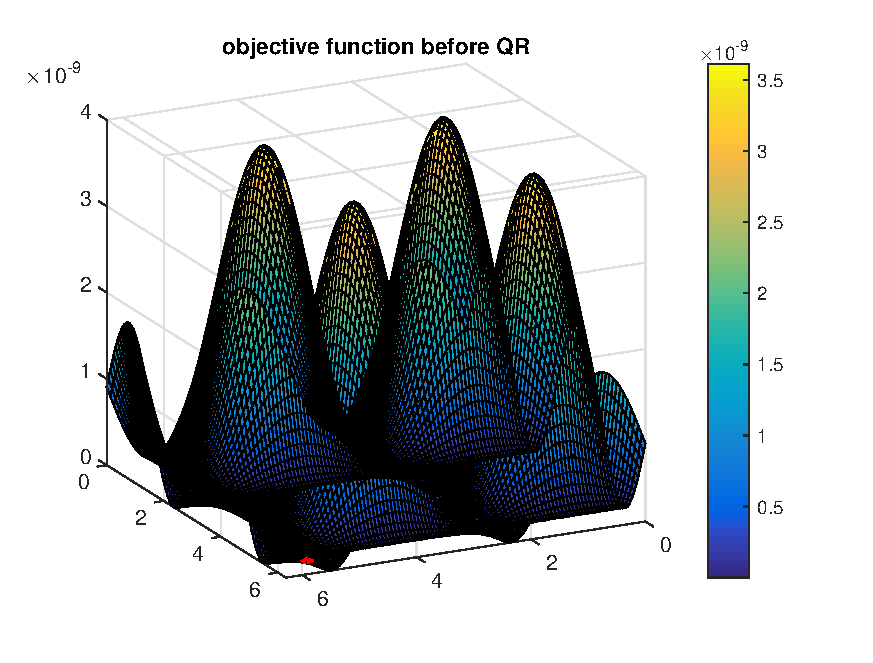
\includegraphics[scale=0.5]{beforeQR2.eps}
% 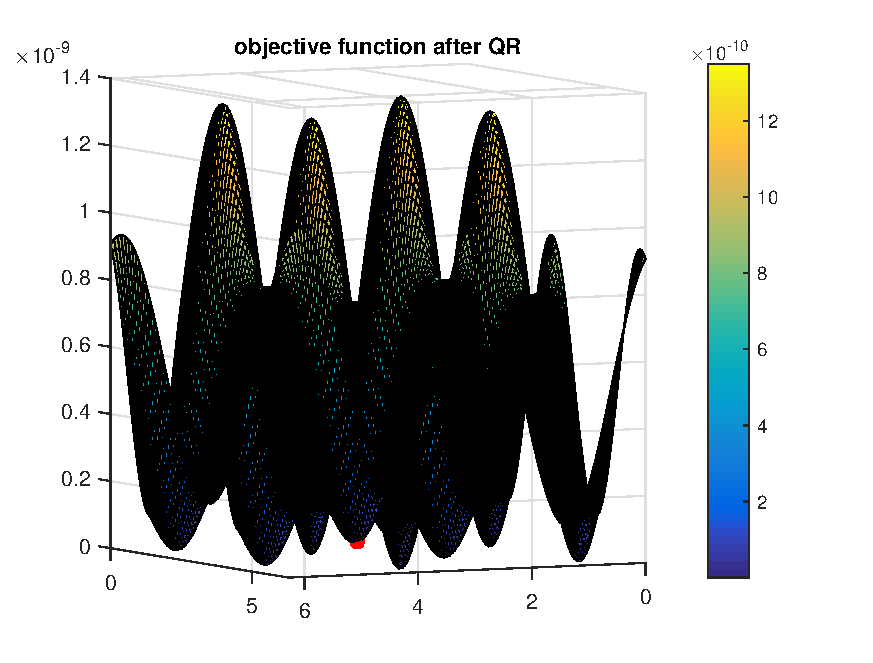
\includegraphics[scale=0.5]{afterQR2.eps}
% \caption{Objective functions before and after QR. The red dot indicates where the global minimum is achieved.}
% \label{QReffect}
%\end{figure}%

\begin{figure}
 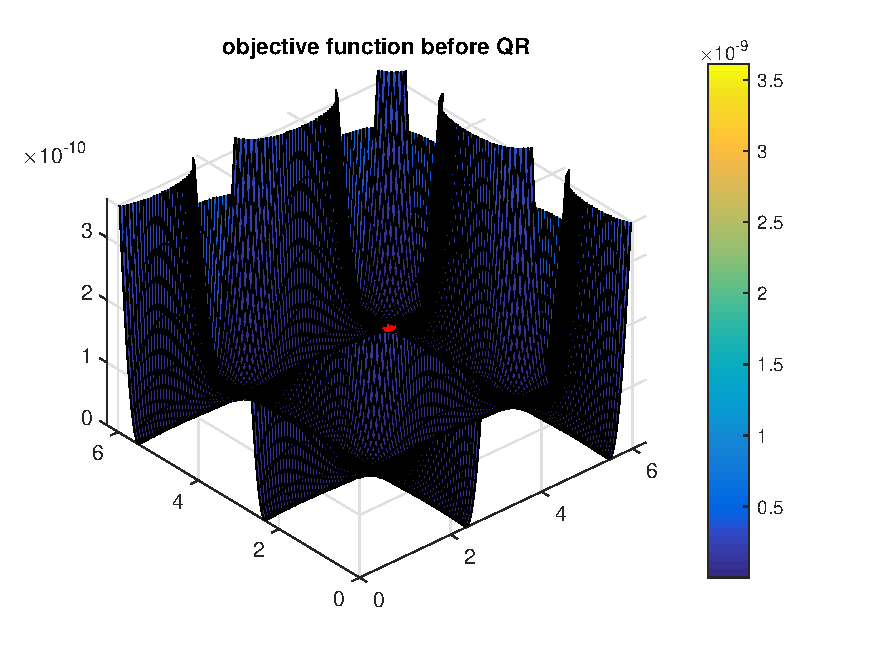
\includegraphics[scale=0.5]{beforeQR3.eps}
 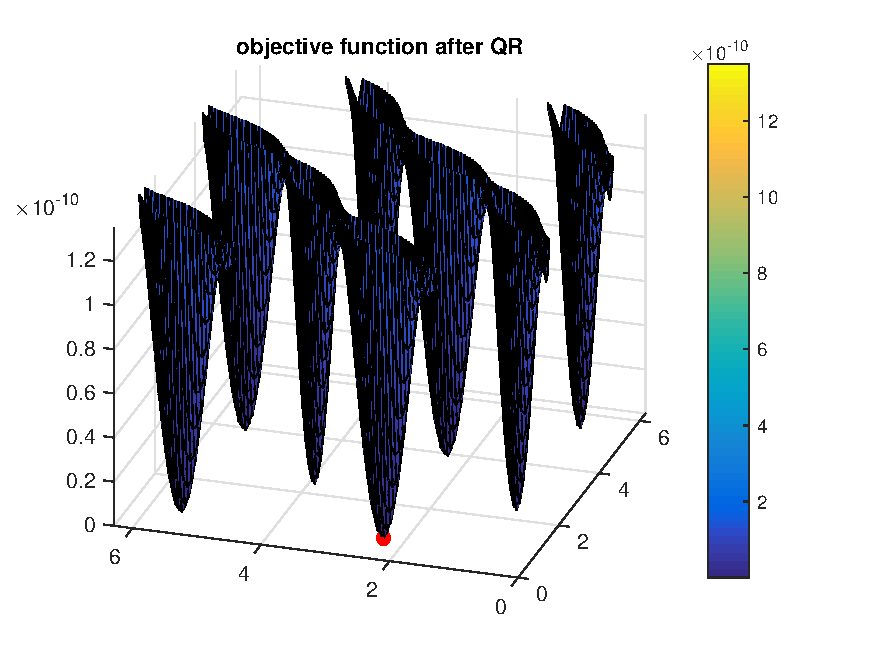
\includegraphics[scale=0.5]{afterQR3.eps}
 \caption{A zoomed-in version of the objective functions before and after applying QR. The red dot indicates where the global minimum is achieved.}
 \label{QReffect}
\end{figure}%

\section{Numerical Results}

In this section,  we present several numerical results to demonstrate the accuracy and robustness of our method. As our stability analysis suggests, it is important to select an appropriate index set so the conditions listed in our stability analysis are satisfied. Since we are using an optimization approach, we can take a larger shift index set for the shifts than the minimum number of shifts that is required by our stability analysis. Thus, even though the stability constant in our stability theorem may be large for minimum shift index set (e.g. $N = d$ for the $d$-signal instantaneous case), one can still get a reasonably accurate recovery. In our numerical implementation, we choose a shift index set to be ${\cal{I}} = \{ n \; | \; 0 \leq n \leq 10 \}$ in the instantaneous case and ${\cal{I}} = \{ n \; |  \; -200 \leq n \leq 200\}$ in the convolutive case with $q=5$ and $\tau=9$. 

We also compare the performance of our method with that of the analytic method (section 5.2 of \cite{Xin14}) based on second order statistics, as well as with the Info-Max method that uses information of speech probability distribution. We do not compare our method with the Jade method \cite{Cardoso93} since this method is limited to instantaneous mixtures only. 
The Info-Max method has been investigated by several authors, see, e.g., \cite{Bell95} and Chapter 5 of \cite{Xin14}. The analytic method is designed for the 2-signal instantaneous case by writing
$B = \begin{bmatrix}       \cos(\theta)  & \sin(\theta) \\      \cos(\phi)   &  \sin(\phi)
\end{bmatrix} ,$ and solving for $\theta$ and $\phi$ analytically from
$\EE [ v_1(t) v_2(t-n) ] = 0$ ($n=1,2$).

This comparison shows that our method can indeed perform better than the analytic de-correlation method (section 5.2, \cite{Xin14}) and the Info-Max method, especially when the mixing matrix is degenerate. 
Our numerical results confirm our theoretical findings. We consider both the instantaneous model and the convolutive model. In the instantaneous case, we consider both the two-signal case and the three-signal case. Of particular interest is the case when the mixing matrix is degenerate. In each of the following examples, we mix together diverse sound signals, consisting of both music and speech. We use diverse speech signals to ensure that our method can accommodate with all types of signals. 

In each test example, the output results include SIRI, which measures the signal-to-interference ratio improvement (see page 145 of \cite{Xin14} for its definition), and the matrix $P$, which confirms Theorem 2.7 and demonstrates the relative accuracy of the recovered signals through the relationship between $v$ and $s$. A larger SIRI indicates greater improvement in the signal. Furthermore, we introduce a quantity $sigmaP$ that
 measures the relative error between $P$ (or its permutation) and the diagonal matrix -- a bigger $sigmaP$ translates to a better recovery. Roughly speaking, $sigmaP = \min_{i} sigmaP_i$, where $sigmaP_i$ is defined as the ratio between the largest element in absolute value and the second largest element in absolute value of the $i$th row of $P$. In all examples, the signal-to-noise ratio $SNR = \frac{P_{signal}}{P_{noise}} $ is about $SNR = 2$.


\vspace{0.1in}
\noindent
{\bf Example 1:}
In the first example, we consider the mixtures of one speech signal with Gaussian noise in the instantaneous case. 
The results obtained by our optimization method are presented in Figure 2. The top row of Figure 2 plots the two mixed signals that are generated using the following mixing matrix
%$A_0 = [ 0.1191  0.8377; 0.9929  0.5461]$. 
\begin{equation} 
A = \begin{bmatrix}

       0.1191  & 0.8377 \\

      0.9929   &  0.5461  

\end{bmatrix} .
\end{equation}
The recovered signals are plotted in the second row, while the original source signals are plotted in the third row of Figure 2. In our optimization method, the shift of $n$ is taken from 0 to 10. Our method gives  SIRI = 52.2411, which indicates that our method gives significant enhancement over the original mixed signals. This is also confirmed by the large value of $sigmaP$ = 382.9470. Finally, the fact that matrix 
\begin{equation} 
P = \begin{bmatrix}      

 -0.6877 &  -0.0016 \\

-0.0018  &  -0.6879 
\end{bmatrix}
\end{equation}
is nearly diagonal gives another confirmation that our optimization method gives an accurate recovery of the original mixed signals without swapping.

We also compare the performance of our method with that of the analytic de-correlation method presented in section 5.2 of \cite{Xin14} (page 142-143). 
As we mentioned earlier, this method of \cite{Xin14} with $n=1,2$ does not take into account explicitly the impact of noise. Although the analytic method in \cite{Xin14} still gives a reasonable enhancement of the mixed signals with SIRI = 18.8522, one can still hear the background noise from the recovered signal. This issue can be shown by the $P$ matrix: 
\begin{equation}
P = \begin{bmatrix}

 1.0000 & 0.0916 \\

0.0000  & 0.9438
\end{bmatrix} .
\end{equation}
One can see that the second component of the first row of $P$ is not small -- about 9.16\% -- indicating that $9.16\%$ of the noise is contained in the recovered speech signal. The value, $sigmaP$ = 10.3055, also confirms this finding. In comparison, our optimization method gives a significantly larger $sigmaP$, 382.9470.


Next, we compare our optimization method with the Info-Max method, which approximates the speech probability distribution function. Using higher order statistics, we observe a considerable improvement over the analytic method of \cite{Xin14} that uses second order statistics. In particular, the Info-Max method gives SIRI = 19.4455, $sigmaP$ = 160.31, and
\begin{equation}
P = \begin{bmatrix}

 -0.0048  & 0.7695 \\

0.9149  & -0.0027
\end{bmatrix} .
\end{equation}
It is interesting to note that the SIRI value does not give an adequate description of the improvement of the Info-Max method over the second order analytic method \cite{Xin14}. The $sigmaP$ value seems to be a better indicator. Note that our optimization method outperforms the Info-Max method in this case by a factor of 2.4.


\begin{figure}[ht!]
     \begin{center}
%
        \subfigure[First Mixture]{%
            \label{fig:first}
            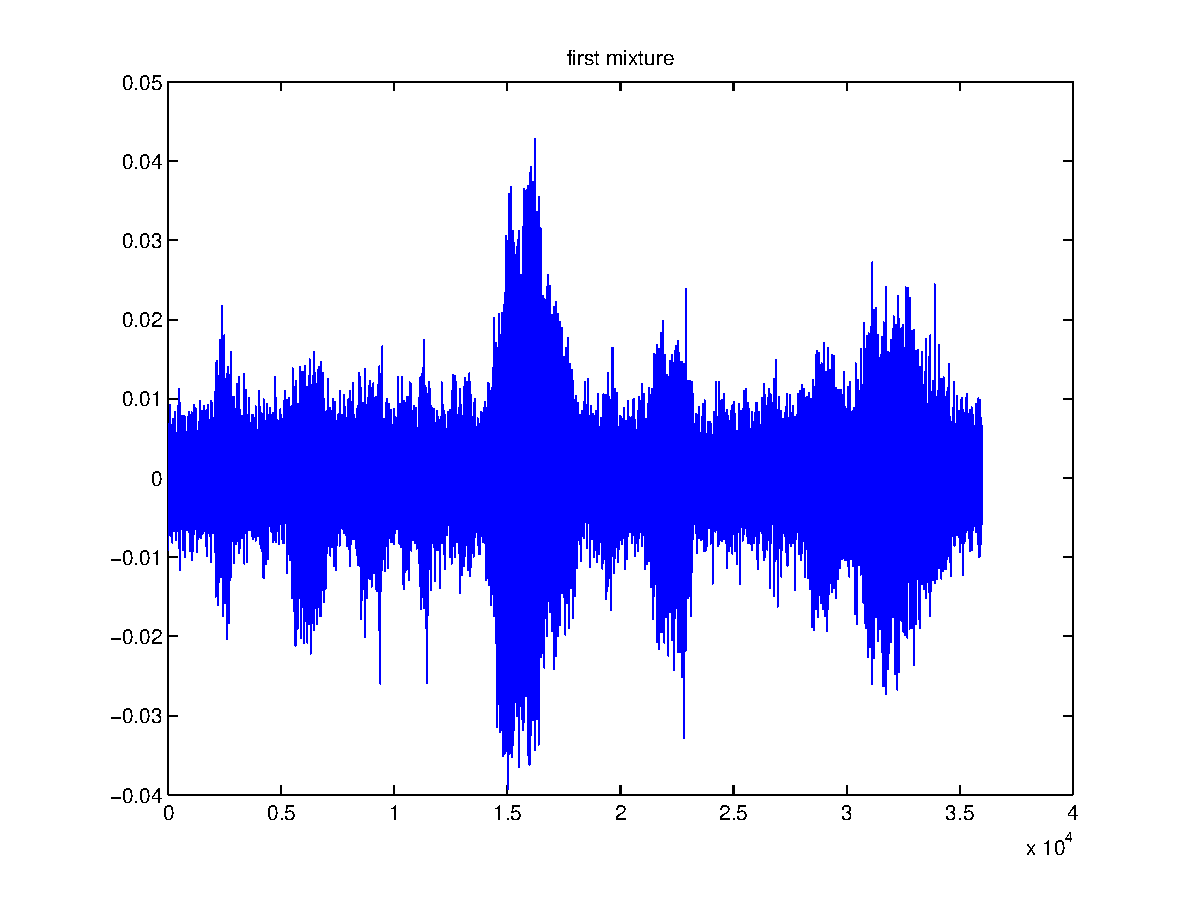
\includegraphics[width=0.4\textwidth]{3-Instantaneous-with-Noise-Optimization/mixture-1.eps}
        }%
        \subfigure[Second Mixture]{%
           \label{fig:second}
           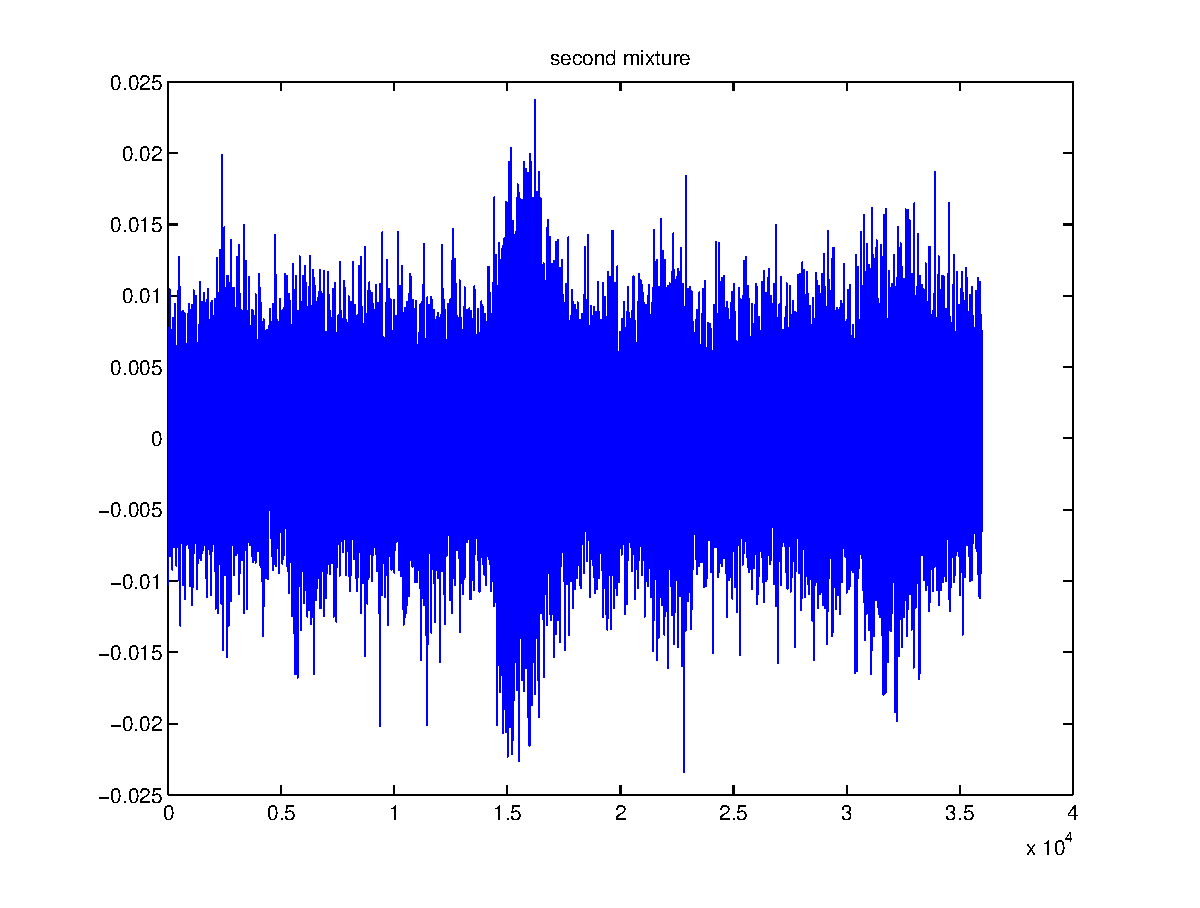
\includegraphics[width=0.4\textwidth]{3-Instantaneous-with-Noise-Optimization/mixture-2.eps}
        } \\
 \subfigure[First Recovered Signal]{%
            \label{fig:first}
            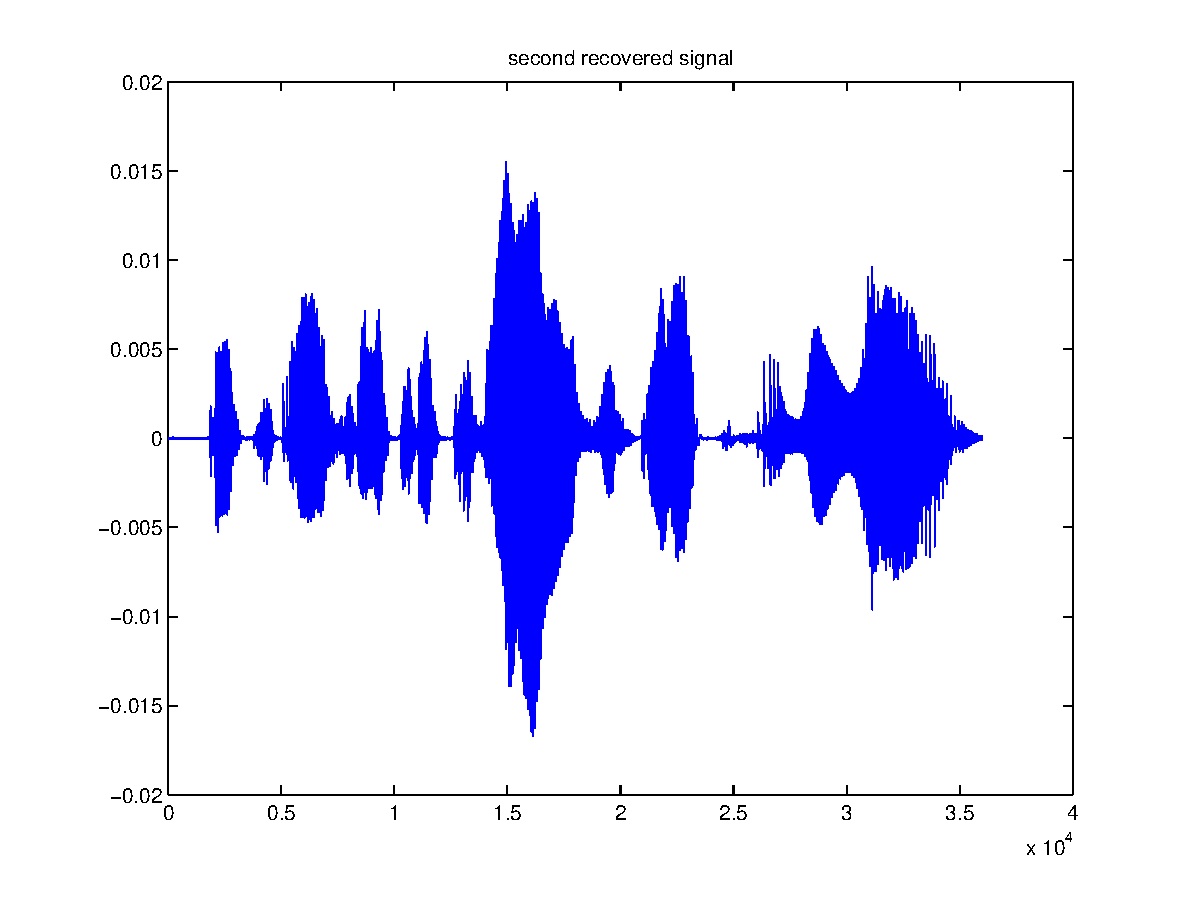
\includegraphics[width=0.4\textwidth]{3-Instantaneous-with-Noise-Optimization/recovered-signal-2.eps}
        }%
        \subfigure[Second Recovered Signal]{%
           \label{fig:second}
           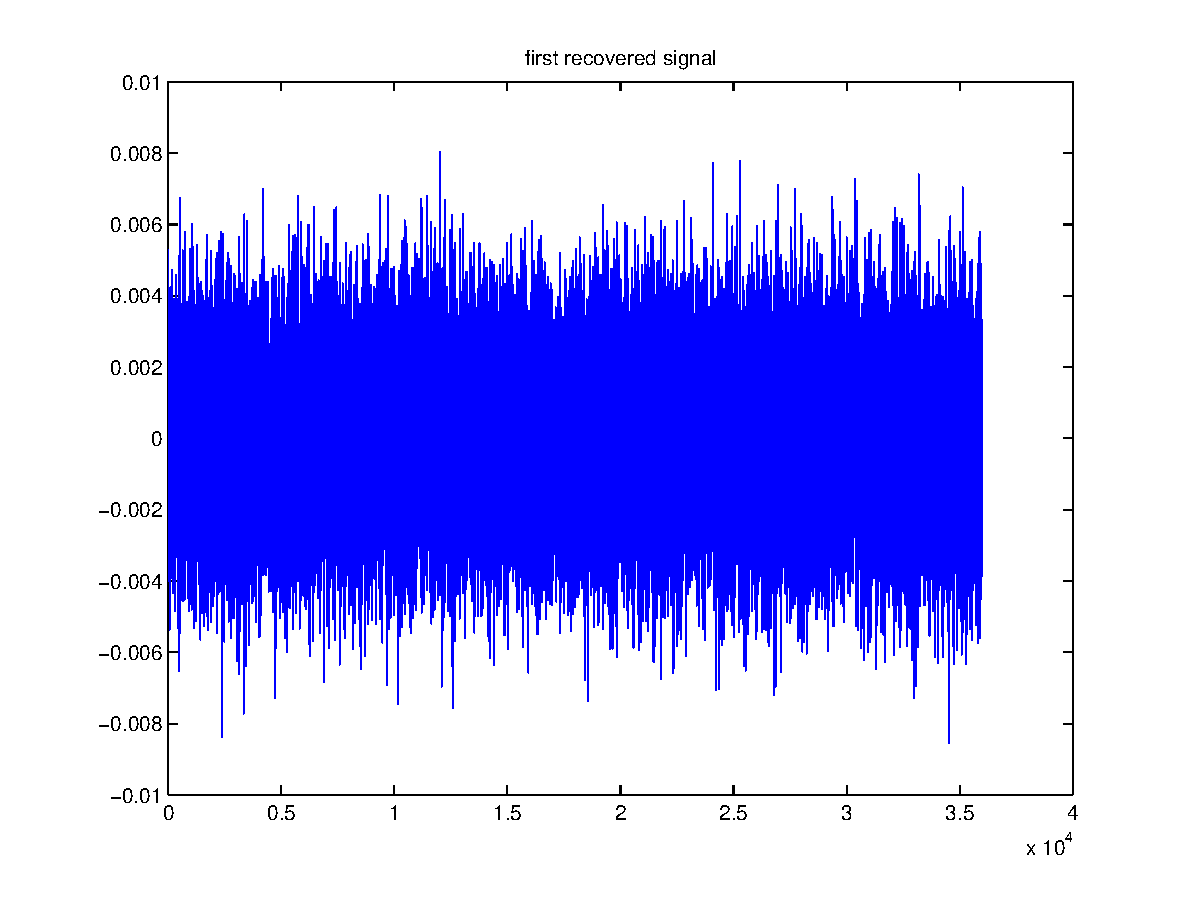
\includegraphics[width=0.4\textwidth]{3-Instantaneous-with-Noise-Optimization/recovered-signal-1.eps}
        } 
        \subfigure[First Source Signal]{%
            \label{fig:first}
            \includegraphics[width=0.4\textwidth]{3-Instantaneous-with-Noise-Optimization/clean-signal-1.eps}
        }%
        \subfigure[Second Source Signal]{%
           \label{fig:second}
           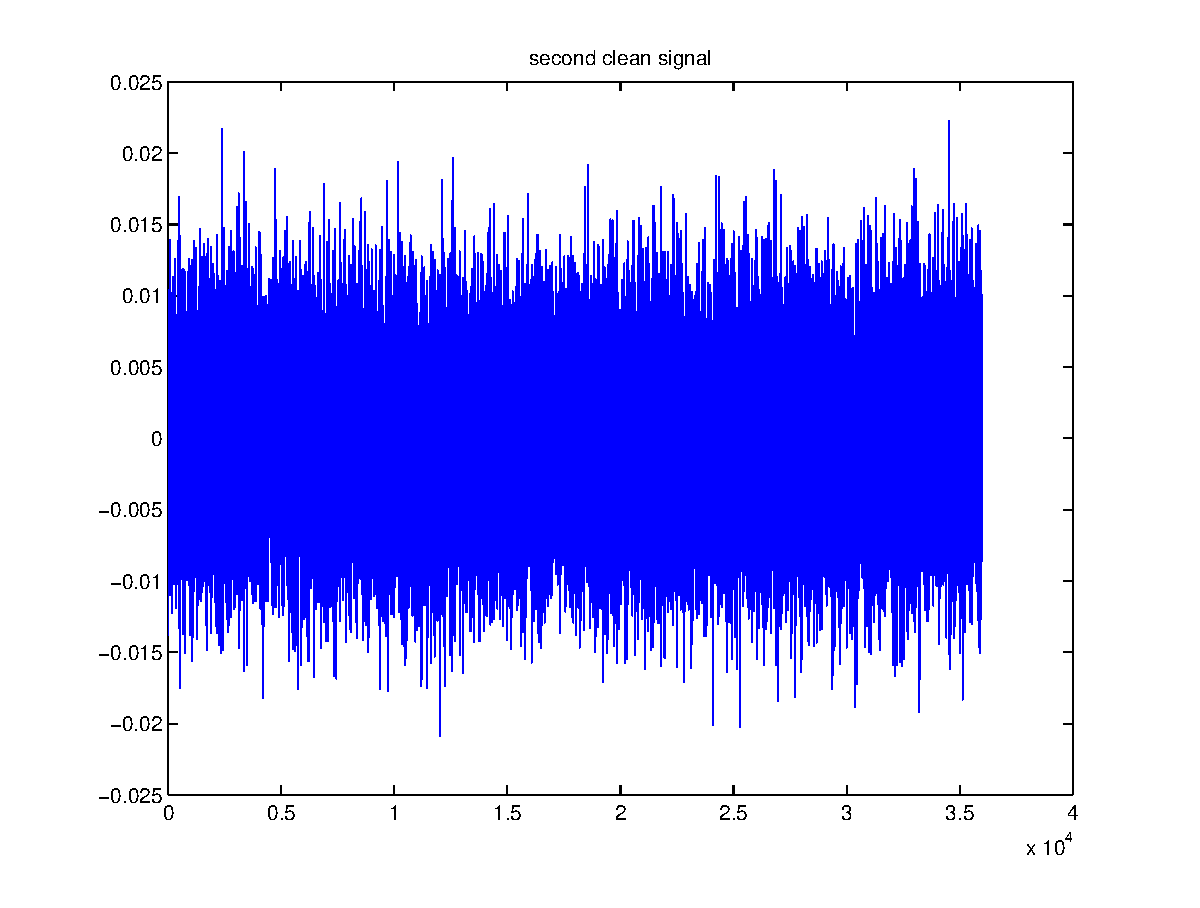
\includegraphics[width=0.4\textwidth]{3-Instantaneous-with-Noise-Optimization/clean-signal-2.eps}
        } \\

    \end{center}
    \caption{%
        This is the instantaneous case where we have a regular signal and a signal composed of random noise. The computation is performed using our optimization method with shifts $n$ taken from 0 to 10. Our method gives
        SIRI = 52.2411 and
%$cond(A)$ = 2.5154, $C_s$ = 1.0820e+08, $det B$ = -0.6890,
 $sigmaP$ = 382.9470. 
%$P$ = [-0.6877  -0.0016; -0.0018  -0.6879], $A_0$ = [0.1191  0.8377; 0.9929  0.5461].
     }%
   \label{fig:subfigures}
\end{figure}

To test the robustness of our method, we randomly generated 100 mixing matrices to produce the measurements for one speech signal mixed with Gaussian noise. We also documented the average $sigmaP$ value for all methods. We use $sigmaP1$ to denote the $sigmaP$ value for our method, $sigmaP2$ for the Info-Max method, and $sigmaP3$ for the analytic method.

The results obtained by our optimization method are presented in Figure 3.
As we can see from the left subplot of Figure 3, the $sigmaP$ for our method is 328.8, the $sigmaP$ value for the Info-Max method is 108.8, and the $sigmaP$ value for the analytic method is 10.4.

In the previous computation, the shift indices for the analytic method were $n=1, 2$. As we have shown in Section 2.5, due to the special property of Gaussian noise, we should take one of the shift indices to be $n=0$ and take the other other shift index to be non-zero. In the right subplot of Figure 3, we repeat the same computation by taking the shift indices for the analytic method to be $n=0,1$. The corresponding $sigmaP$ value improved significantly, increasing from 10.4  to a value of 143.5.

\begin{figure}
 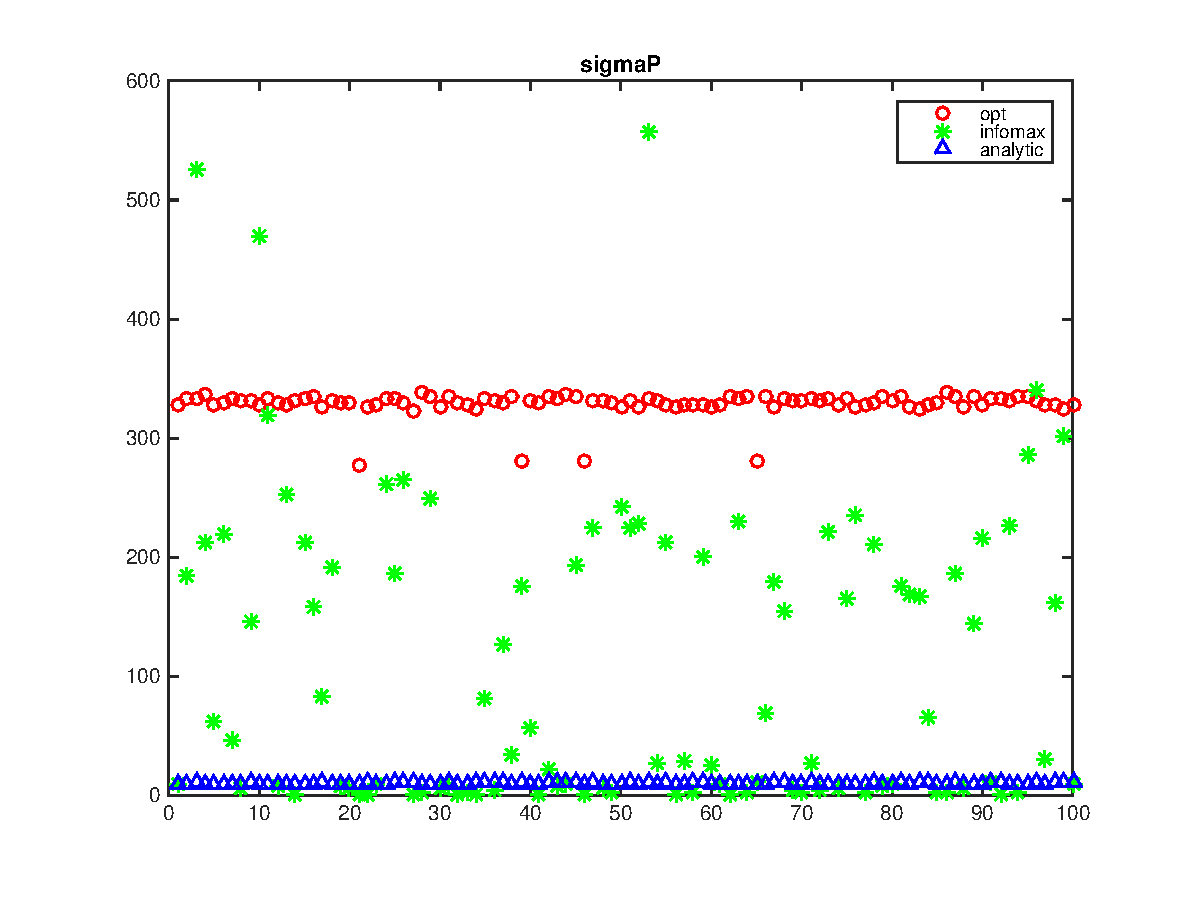
\includegraphics[scale=0.4]{0-Beijing/1sig1noiseOptimization/sigmaP-speech.eps}
 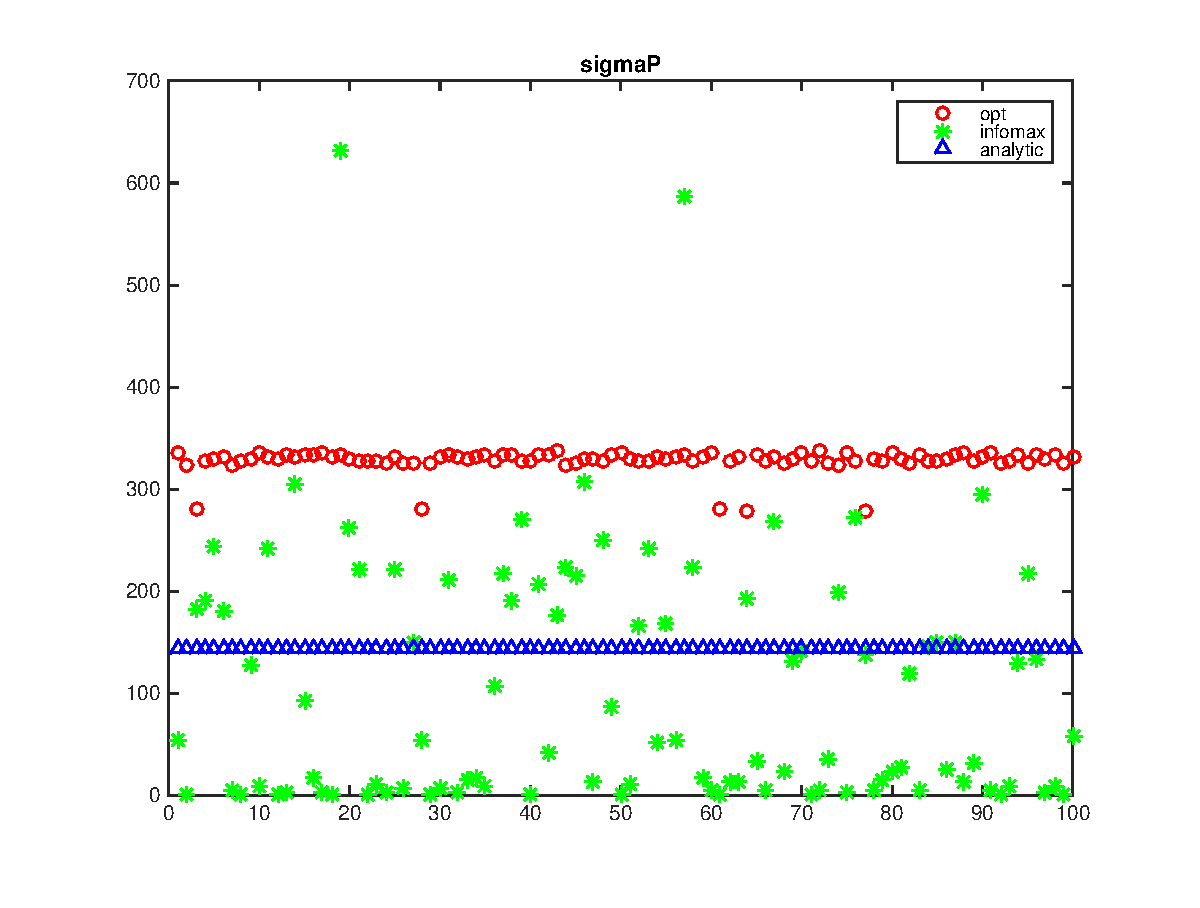
\includegraphics[scale=0.4]{0-Beijing/1sig1noiseOptimization/sigmaP-speech-01shift.eps}
\caption{One speech signal mixed with noise. Comparison of our optimization method, the Info-Max method and the analytic method. Left subplot: $sigmaP1 = 328.8$, $sigmaP2 = 108.8$,
$sigmaP3 = 10.4$, $n=1,2$ for the analytic method. Right subplot: $sigmaP1 = 327.8$, $sigmaP2 = 103.8$, $sigmaP3 = 143.5$, $n=0,1$ for the analytic method. }
 \label{Example 1}
\end{figure}%

\vspace{0.1in}
\noindent
{\bf Example 2:}
In this example, we consider the three-signal mixtures in the instantaneous case. We use two speech signals mixed with a Gaussian noise signal. The mixing matrix $A$ is given by
%$A_0$ = [ 2.0795  -1.2925  -0.3978; 0.2554  -0.5062   1.1136; -0.953  1.8890  -0.2922]
\begin{equation}
A = \begin{bmatrix}
2.0795 &  -1.2925  & -0.3978 \\ 
0.2554 &  -0.5062 & 1.1136 \\
-0.953 & 1.8890 &  -0.2922
\end{bmatrix} .
\end{equation}
We compare the performance of our optimization method with that of the Info-Max method. The results obtained by our optimization method are given in Figure 4. Again, we plot the mixtures in the first row, the recovered signals in the second row, and the original source signals in the third row, which are in Figure 4. Our method gives SIRI = 20.6428, $sigmaP$ = 43.4990, and
%$P$ = [0.9825  0.0226  -0.0054; -0.0125  1.0119 -0.0011; -0.0037  0.0073  0.9979], 
\begin{equation}
P = \begin{bmatrix}
0.9825 &  0.0226 & -0.0054 \\
-0.0125 &  1.0119 & -0.0011 \\
-0.0037 & 0.0073 &  0.9979
\end{bmatrix} .
\end{equation}
Although the results are not as accurate as those of the two-signal case, the recovered signals still have reasonable accuracy. 

We tend to believe that a main factor in the decrease of accuracy of the three-signal case, as well as the convolutive case, is due to the performance of the global optimization algorithm in the Matlab code. In the three-signal instantaneous case and the convolutive case, the number of unknowns increases significantly, making it extremely difficult to find the global minimum of our non-convex energy functional. In many cases, the algorithm only returns a local minimum instead of a global minimum. The ability to design an even more effective global optimization method will be key to our proposed approach, a subject that we will investigate in the future.

We have also compared this method with the Info-Max method using the same mixing matrix and data. The Info-Max method gives SIRI = 17.4613, $sigmaP = 23.9777$, and
%$P$ = [1.3979   0.0583  -0.0008; 0.0003   0.0092   1.0318; 0.0143   1.1425   0.0083] 
\begin{equation}
P = \begin{bmatrix}
1.3979  &  0.0583  & -0.0008 \\
0.0003  &  0.0092 &  1.0318 \\
0.0143  & 1.1425  &  0.0083
\end{bmatrix} .
\end{equation}
As in the two-signal case, we can see that our optimization method still outperforms the Info-Max method for the three-signal case by about a factor of 2 if we compare the values of $sigmaP$ obtained by the two approaches.

This numerical experiment demonstrates that our global optimization method can, with reasonable accuracy, recover the two source signals mixed with noise. Not only do our results demonstrate an accurate recovery of generic sound signals, but we also demonstrate that we can handle the impact of Gaussian noise.
The small values of the off-diagonals in the $P$ matrix solidify our claims that our three-signal global optimization method can accurately recover source signals.

\begin{figure}[ht!]
     \begin{center}
%
        \subfigure[First Mixture]{%
            \label{fig:first}
            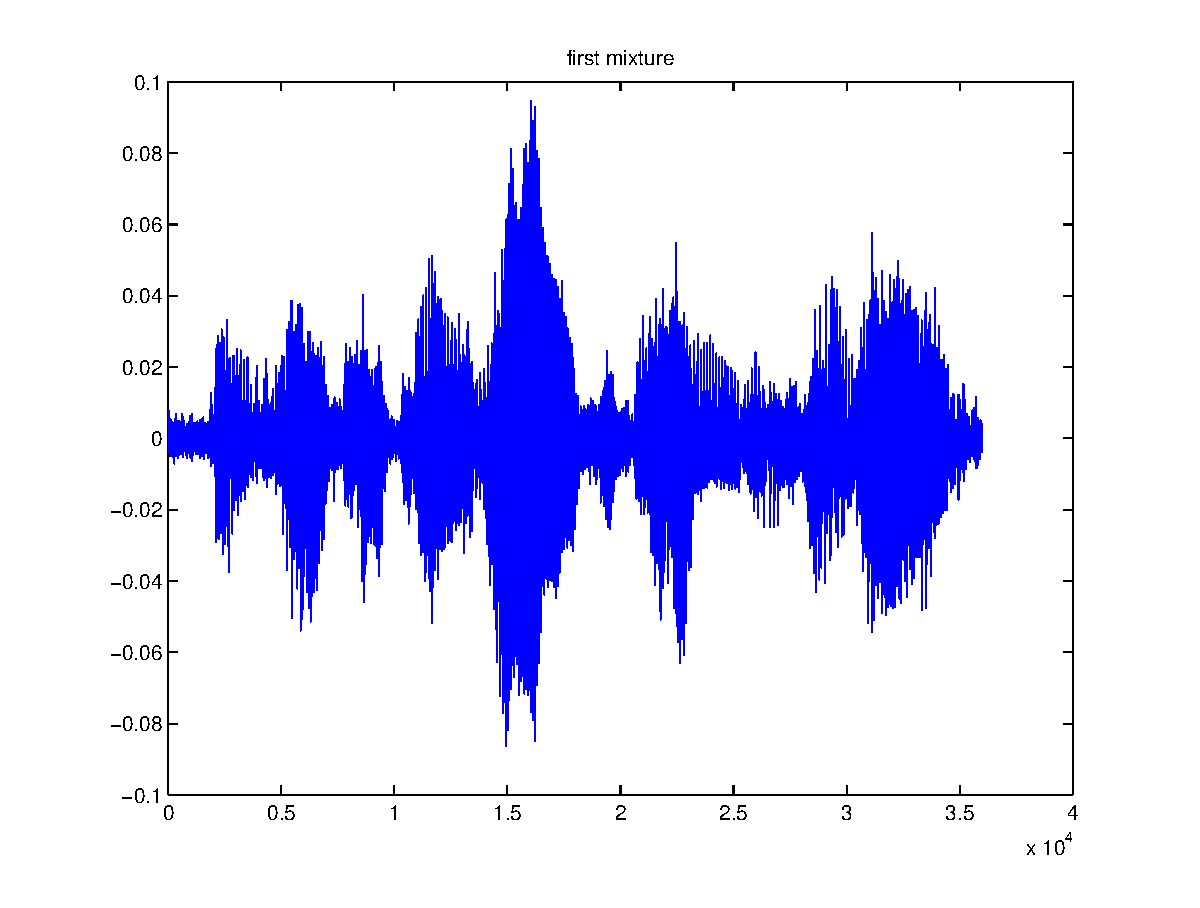
\includegraphics[width=0.33\textwidth]{5-Instantaneous-Three-Source-Separation-Global-Optimization-with-Noise/mixture-1.eps}
        }%
        \subfigure[Second Mixture]{%
           \label{fig:second}
           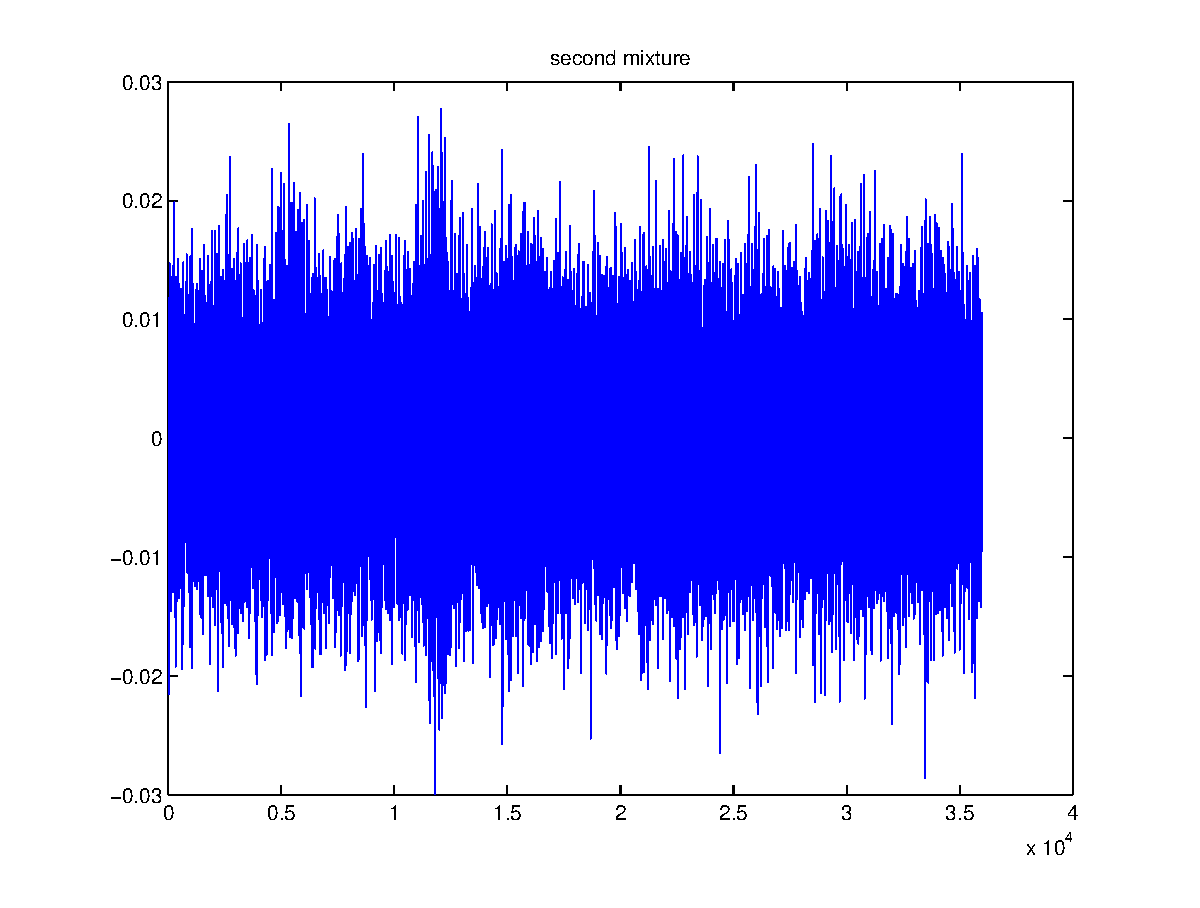
\includegraphics[width=0.33\textwidth]{5-Instantaneous-Three-Source-Separation-Global-Optimization-with-Noise/mixture-2.eps}
        }%
       \subfigure[Third Mixture]{%
            \label{fig:third}
            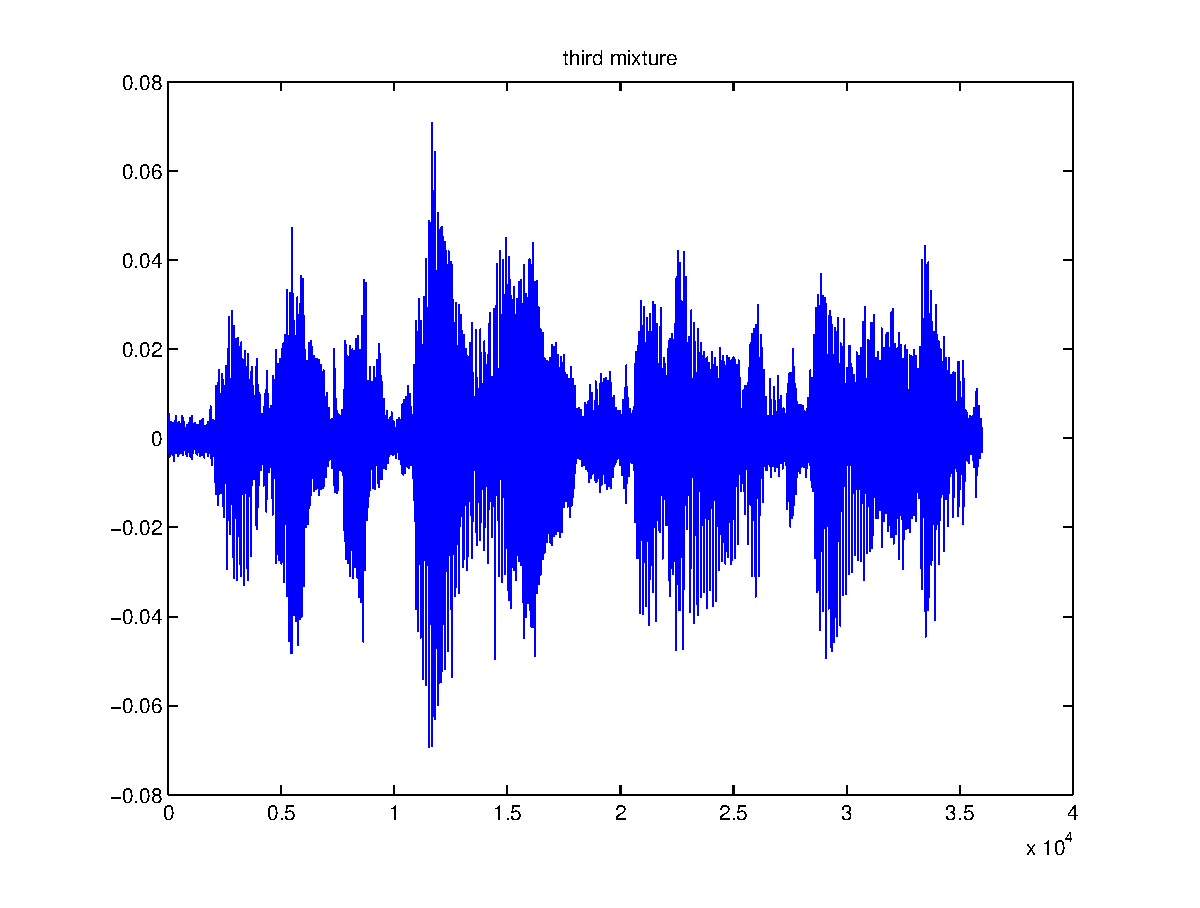
\includegraphics[width=0.33\textwidth]{5-Instantaneous-Three-Source-Separation-Global-Optimization-with-Noise/mixture-3.eps}    
        } \\
 \subfigure[First Recovered Signal]{%
            \label{fig:first}
            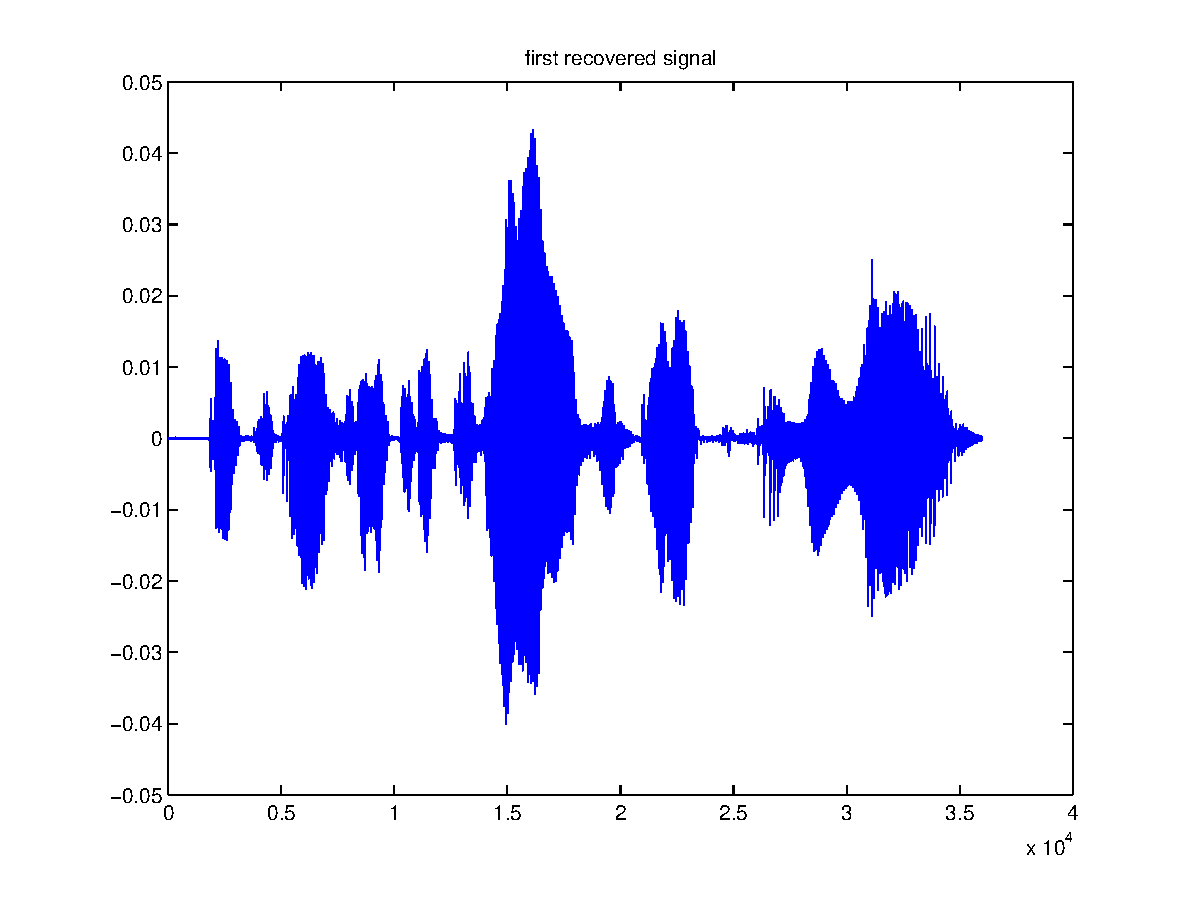
\includegraphics[width=0.33\textwidth]{5-Instantaneous-Three-Source-Separation-Global-Optimization-with-Noise/recovered-signal-1.eps}
        }%
        \subfigure[Second Recovered Signal]{%
           \label{fig:second}
           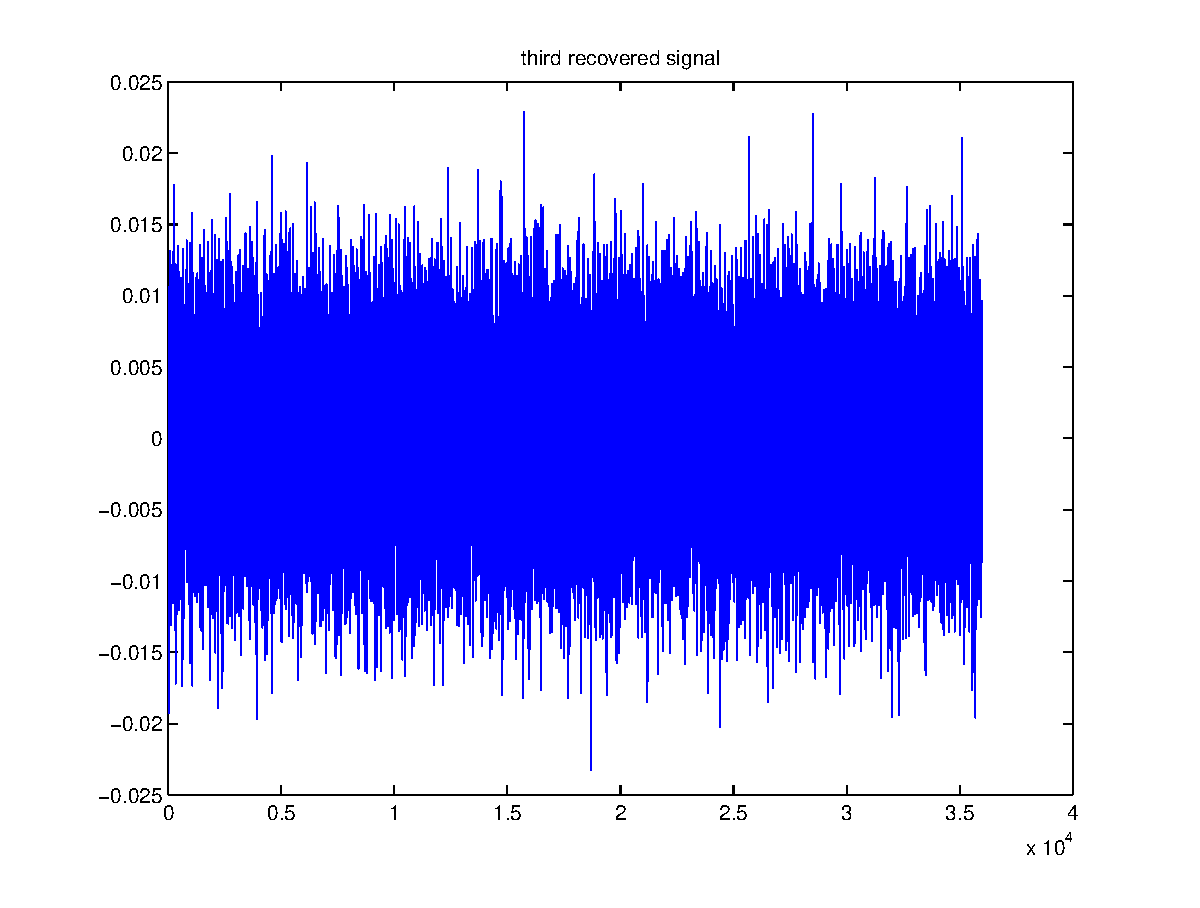
\includegraphics[width=0.33\textwidth]{5-Instantaneous-Three-Source-Separation-Global-Optimization-with-Noise/recovered-signal-3.eps}
        }%
        \subfigure[Third Recovered Signal]{%
            \label{fig:third}
            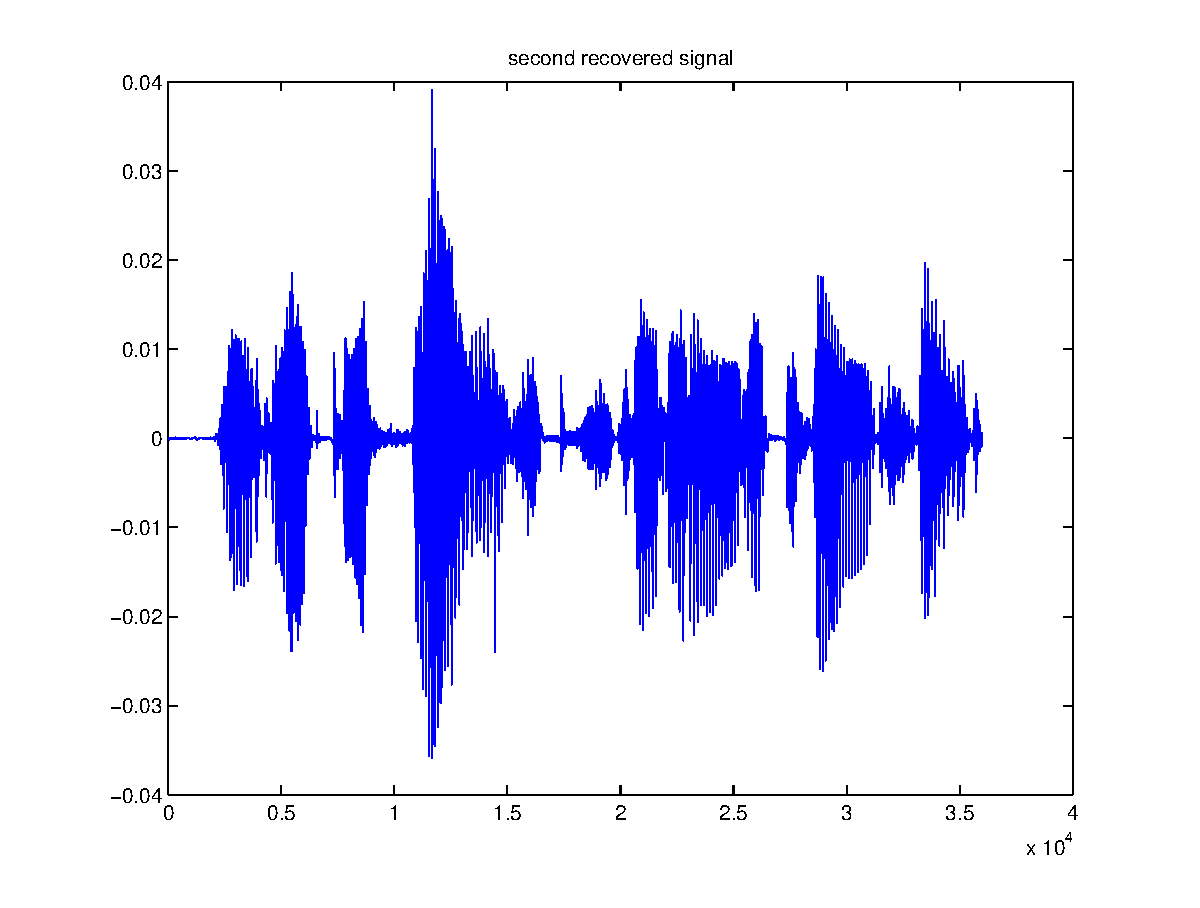
\includegraphics[width=0.33\textwidth]{5-Instantaneous-Three-Source-Separation-Global-Optimization-with-Noise/recovered-signal-2.eps}   
        } \\ 
        \subfigure[First Source Signal]{%
            \label{fig:first}
            \includegraphics[width=0.33\textwidth]{5-Instantaneous-Three-Source-Separation-Global-Optimization-with-Noise/clean-signal-1.eps}
        }%
        \subfigure[Second Source Signal]{%
           \label{fig:second}
           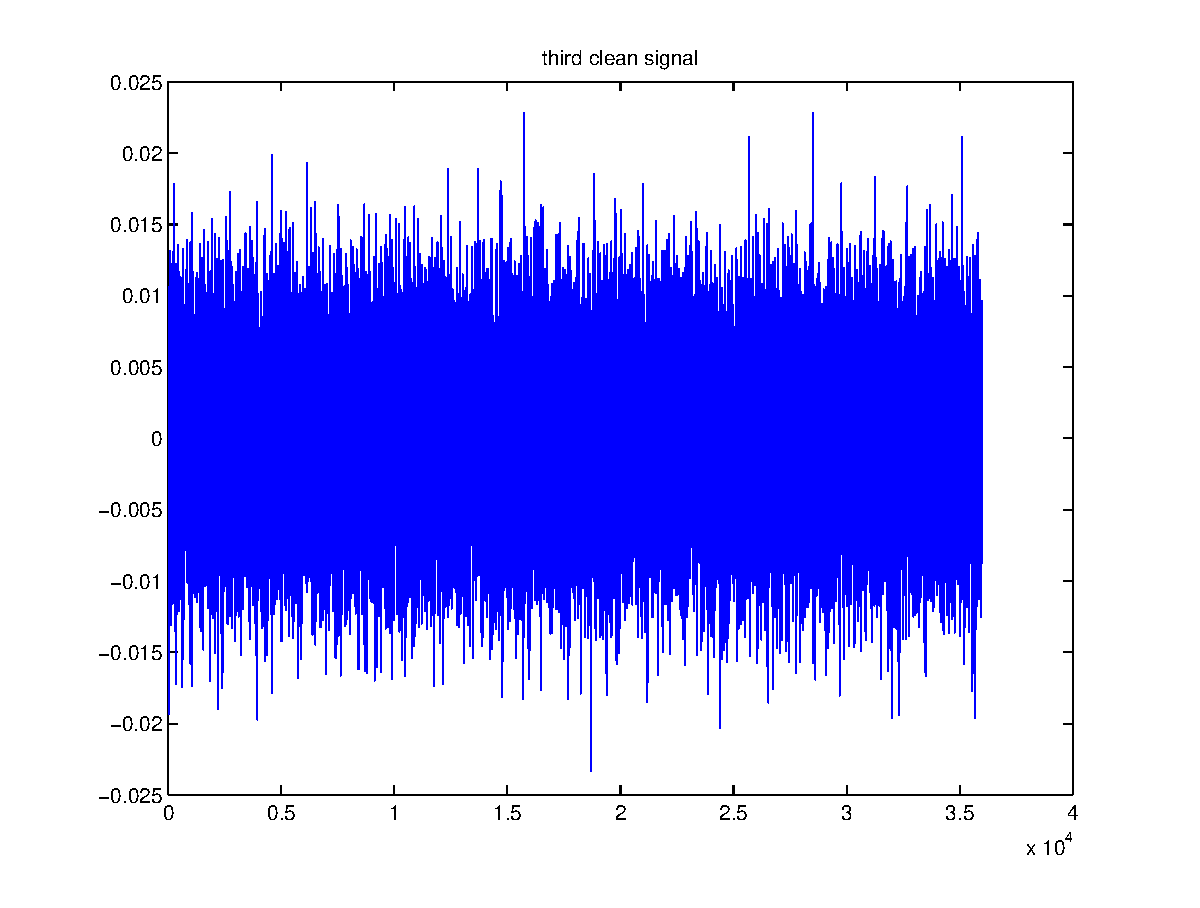
\includegraphics[width=0.33\textwidth]{5-Instantaneous-Three-Source-Separation-Global-Optimization-with-Noise/clean-signal-3.eps}
        }%
        \subfigure[Third Source Signal]{%
            \label{fig:third}
            \includegraphics[width=0.33\textwidth]{5-Instantaneous-Three-Source-Separation-Global-Optimization-with-Noise/clean-signal-2.eps}    
        } \\

    \end{center}
    \caption{
   This is the instantaneous case where we explore the three-signal case, where two sources are regular speech signals and one source is a random noise signal. To recover the signals, we use our global optimization method. Our method gives SIRI = 20.6428 and
% $cond(A)$ = 4.8570, $C_s$ = 5.2745e+05, $det B$ = -0.3555, 
$sigmaP$ = 43.4990. 
%$P$ = [0.9825  0.0226  -0.0054; -0.0125  1.0119 -0.0011; -0.0037  0.0073  0.9979], $A_0$ = [ 2.0795  -1.2925  -0.3978; 0.2554  -0.5062   1.1136; -0.953  1.8890  -0.2922]. 
     }%
   \label{fig:subfigures}
\end{figure}

\vspace{0.1in}
\noindent
{\bf Example 3:}
Next, we consider the two-signal instantaneous case with a degenerate mixing matrix $A$. Again, we consider the case where we have one regular speech signal mixed with random noise. Our numerical results will confirm the theoretical results obtained in Section 4 -- that we can still obtain accurate recovery of the mixed signals even when the mixing matrix $A$ is degenerate. 

In Figure 5, we plot the results obtained by our optimization method. The layout is exactly the same as that of Figure 2. The degenerate matrix $A$ is given by 
\begin{equation}
A = \begin{bmatrix}
0.7071 & 0.7078 \\
 0.7071 &  0.7064
\end{bmatrix} .
\end{equation}
The degree of degeneracy can be measured by its determinant, $det(A) = 0.00607406$. 
Our optimization method gives SIRI = 22.1174, $sigmaP$ = 41.1483, and
\begin{equation}
P = \begin{bmatrix}
1.0031 & 0.0179 \\
 -0.0031 &  0.9821
\end{bmatrix} .
\end{equation}
Given the nature of the degenerate measurement, these results are quite impressive.

We compare our optimization method with the analytic method of \cite{Xin14} with shift $n$ taken from 1 to 2. This method of \cite{Xin14} gives SIRI = 10.3856, 
$sigmaP$ = 9.9176, and
\begin{equation}
P = \begin{bmatrix}
1.0000  &  0.0916 \\
 0.0000 &   0.9084
\end{bmatrix} .
\end{equation}
As one can infer from matrix $P$, there is about 9.16\% of mixture of the background noise in the first recovered source signal. When we play the recovered signal, the effect of the noise is quite noticeable.

I also apply the Info-Max method to this degenerate measurement case.
The Info-Max method gives SIRI = 5.2362, $sigmaP$ = 3.9571, 
and
\begin{equation}
P = \begin{bmatrix}
0.2530 & -0.0202 \\
 0.1096  & 0.4337
\end{bmatrix} .
\end{equation}
As we can see from matrix $P$, about 23\% of the first source signal is still mixed with the second source signal in the recovered second signal. When we play the recovered signals, the mixing of the two signals is quite strong. We have also applied the Info-Max method to many other signals with a degenerate measurement. We found that the Info-Max method typically gives very poor recovery when $A$ is degenerate. 

\begin{figure}[ht!]
     \begin{center}
%
        \subfigure[First Mixture]{%
            \label{fig:first}
            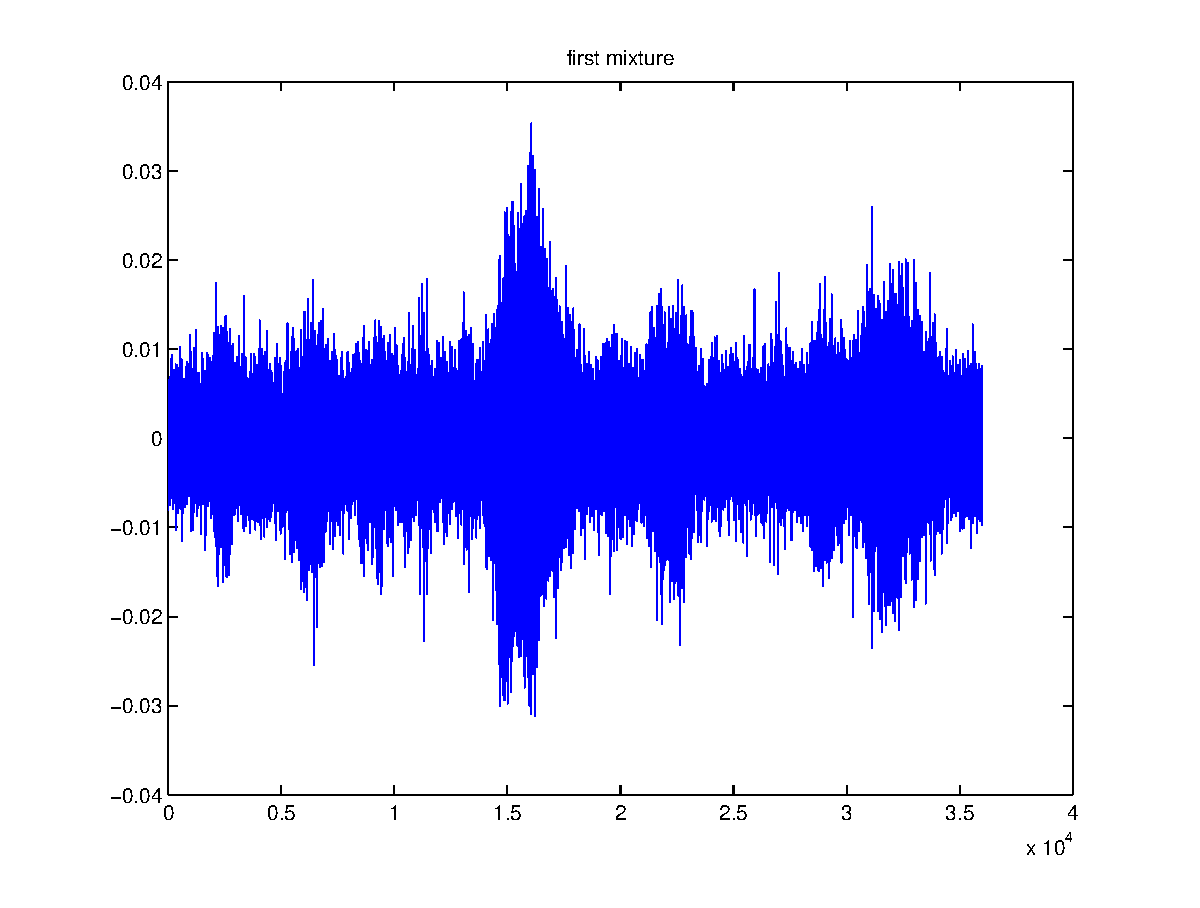
\includegraphics[width=0.4\textwidth]{6-Instantaneous-Degeneracy-Case/Instantaneous-with-Noise-1-to-2/mixture-1.eps}
        }%
        \subfigure[Second Mixture]{%
           \label{fig:second}
           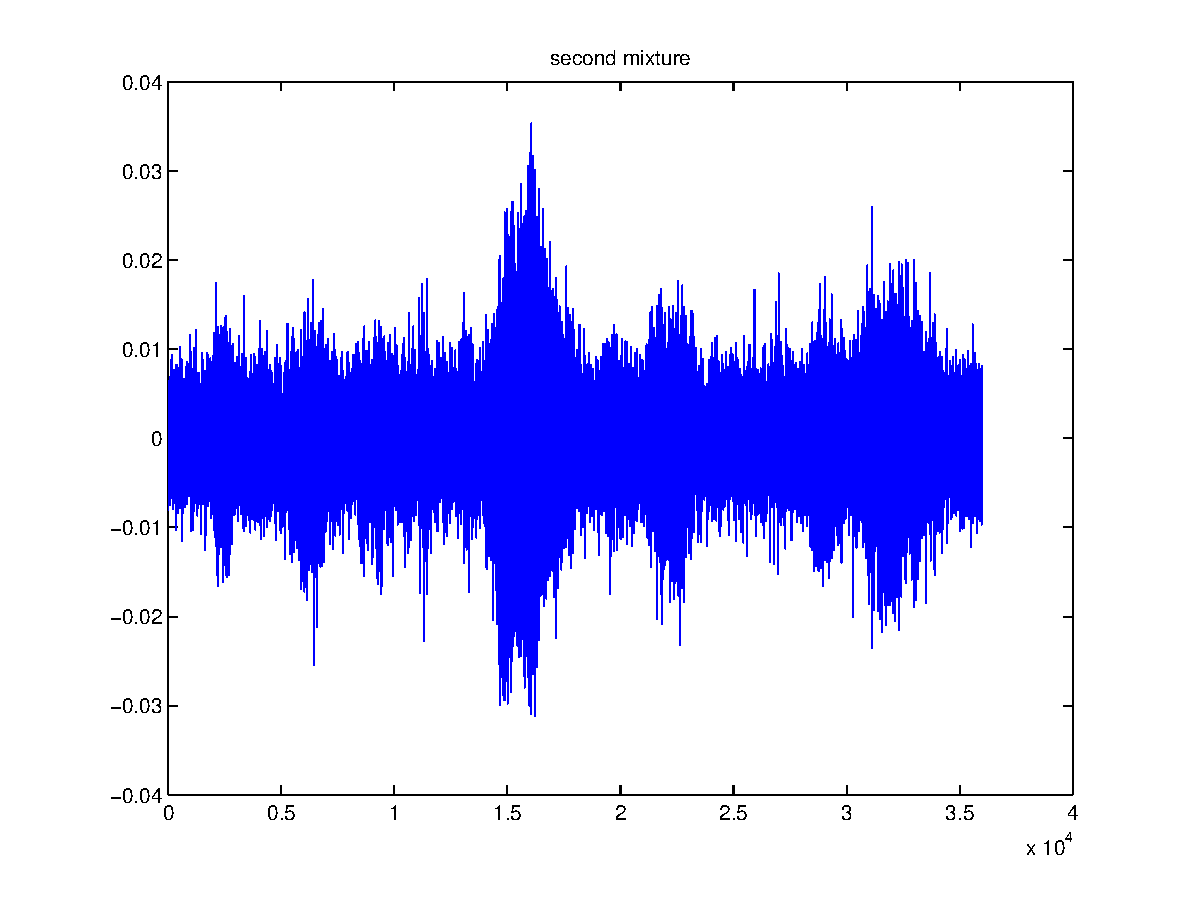
\includegraphics[width=0.4\textwidth]{6-Instantaneous-Degeneracy-Case/Instantaneous-with-Noise-1-to-2/mixture-2.eps}
        } \\
 \subfigure[First Recovered Signal]{%
            \label{fig:first}
            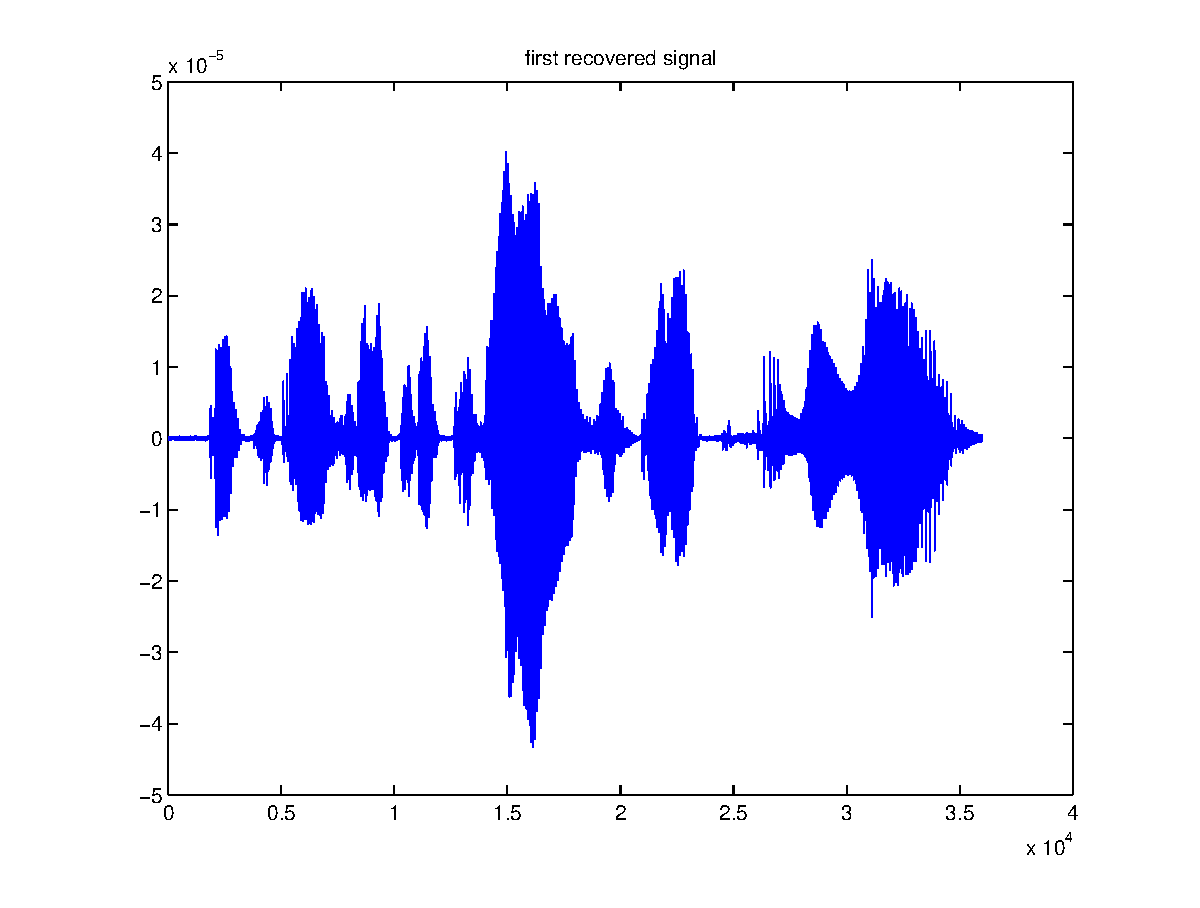
\includegraphics[width=0.4\textwidth]{6-Instantaneous-Degeneracy-Case/Instantaneous-with-Noise-1-to-2/recovered-signal-1.eps}
        }%
        \subfigure[Second Recovered Signal]{%
           \label{fig:second}
           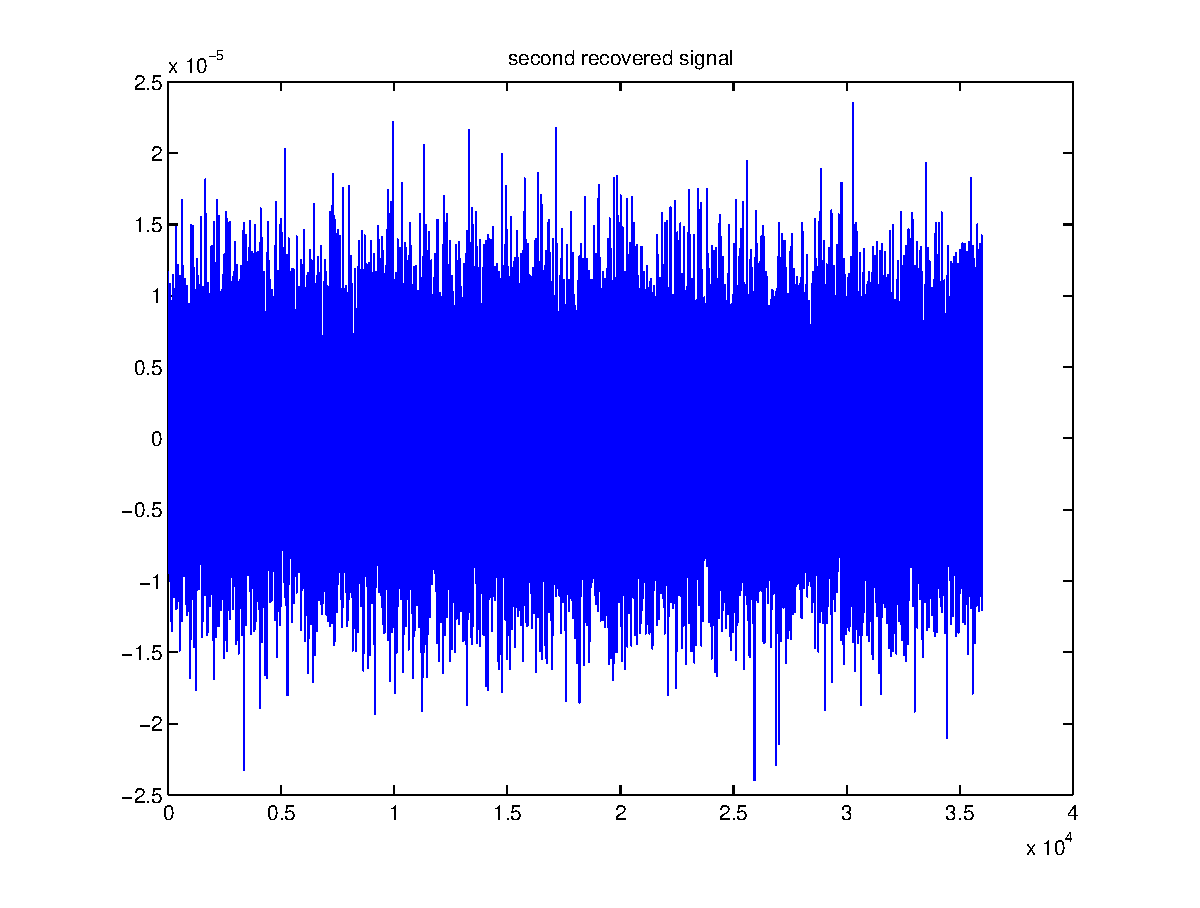
\includegraphics[width=0.4\textwidth]{6-Instantaneous-Degeneracy-Case/Instantaneous-with-Noise-1-to-2/recovered-signal-2.eps}
        } 
        \subfigure[First Source Signal]{%
            \label{fig:first}
            \includegraphics[width=0.4\textwidth]{6-Instantaneous-Degeneracy-Case/Instantaneous-with-Noise-1-to-2/clean-signal-1.eps}
        }%
        \subfigure[Second Source Signal]{%
           \label{fig:second}
           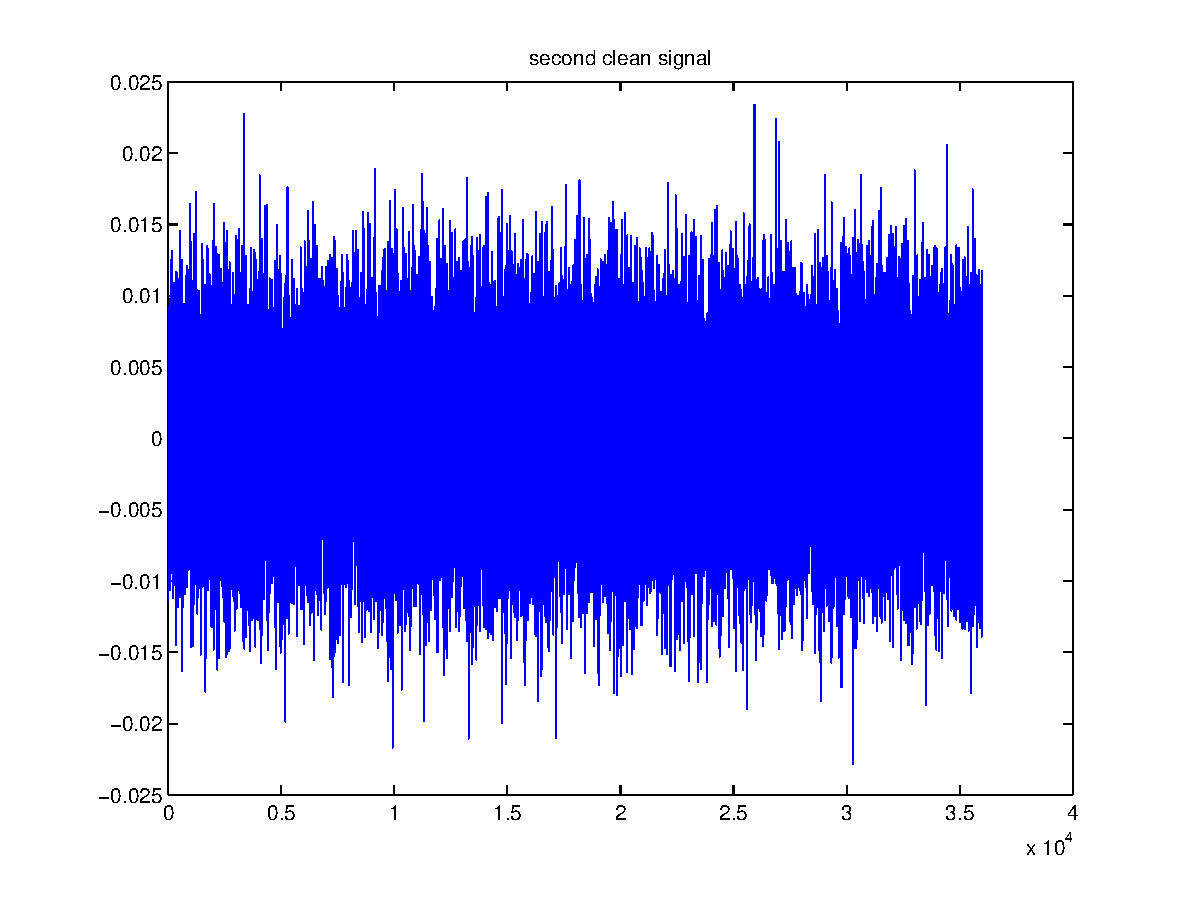
\includegraphics[width=0.4\textwidth]{6-Instantaneous-Degeneracy-Case/Instantaneous-with-Noise-1-to-2/clean-signal-2.eps}
        } \\

    \end{center}
    \caption{%
        This is the instantaneous case where the A matrix is degenerate. 
%The degenerate mixing matrix is given by $A0$ = [0.7071  0.7078; 0.7071  0.7064]. 
We have one regular signal mixed with random noise in the instantaneous setting. Our optimization method gives SIRI = 22.1174 and $sigmaP$ = 41.1483.
% $P$ = [1.0031  0.0179; -0.0031  0.9821]. 
     }%
   \label{fig:subfigures}
\end{figure}

To test the robustness of our method, we randomly generated 100 mixing matrices to produce the degenerate measurements for one speech signal mixed with Gaussian noise. Our numerical results confirm the theoretical results obtained in Section 4.1 -- that we can still obtain accurate recovery of the mixed signals even when the mixing matrix $A$ is degenerate.

In the left subplot of Figure 6, we plot the results obtained by our optimization method.
Our optimization method gives $sigmaP$ = 330.7. The Info-Max method does very poorly for degenerate measurements. Its $sigmaP$ value is only equal to 1. The poor performance of the Info-Max method for degenerate measurements seems quite typical. The analytic method with shift $n=0,1$ performs quite well, giving $sigmaP$ = 142.3. 

\begin{figure}
\begin{center}
 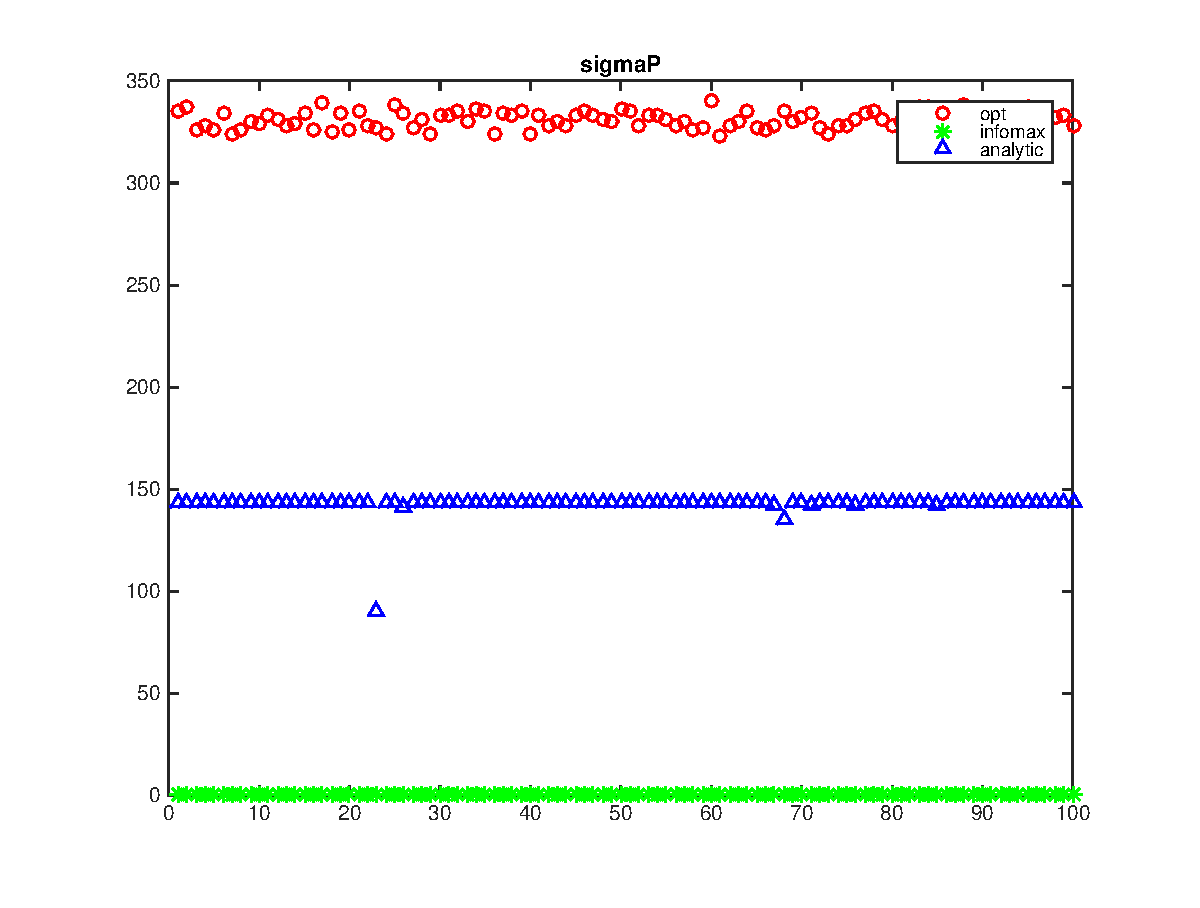
\includegraphics[scale=0.4]{0-Beijing/1sig1noiseOptimization/sigmaP-speech-deg-preQR.eps}
\end{center}
%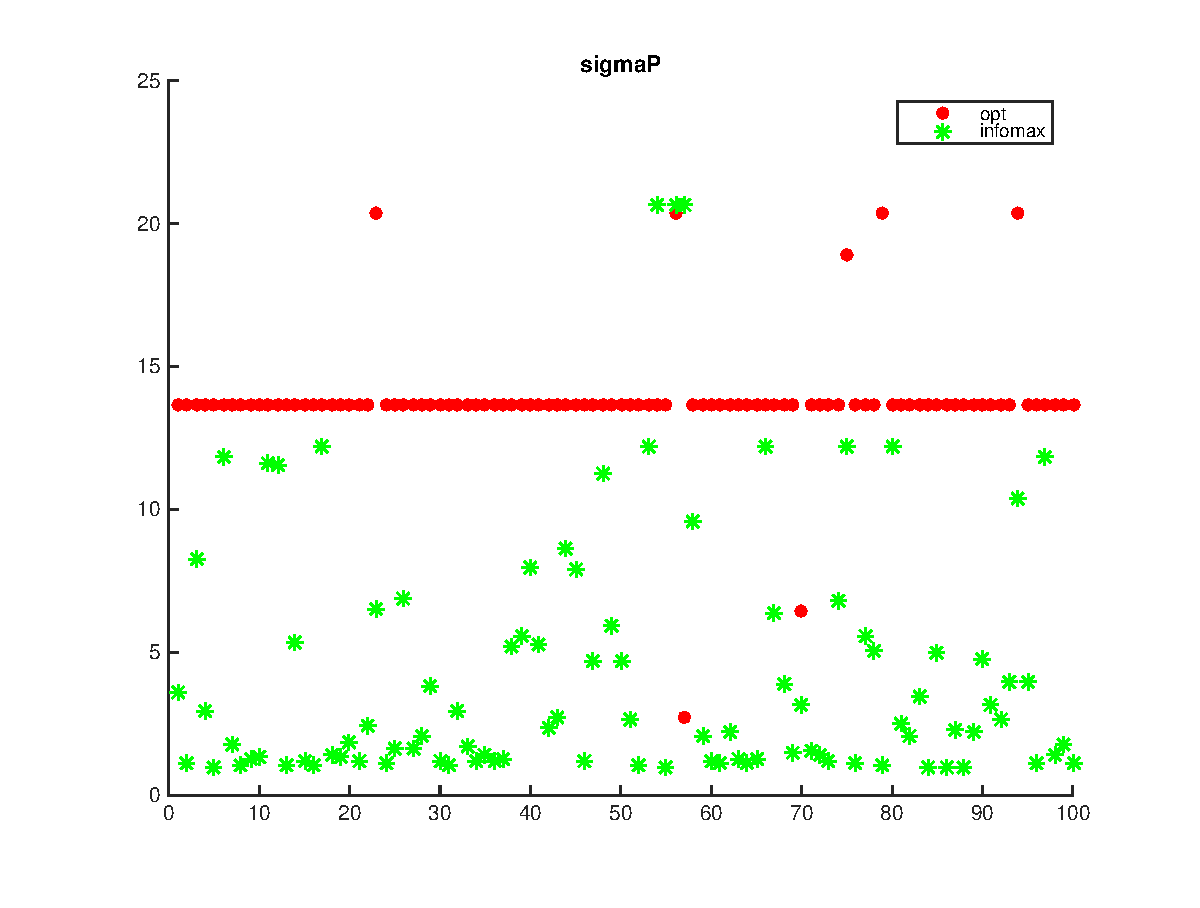
\includegraphics[scale=0.4]{0-Beijing/3by3_2sig1noise_deg/sigmaP-music-reg.eps}
\caption{One speech signal mixed with noise in the degenerate case. 
$sigmaP1 = 330.7$, $sigmaP2 = 1$, and $sigmaP3 = 142.3$.}
 \label{Example 2}
\end{figure}%

\vspace{0.1in}
\noindent
{\bf Example 4:}
Now we test the performance of our optimization method for the more realistic convolutive case. We use the same signals and mixtures as those used in \cite{Xin14}. The results obtained by our global optimization method are presented in Figure 7. The layout is the same as before. Again, the mixed signals are plotted in the first row, the recovered signals in the second row, and the original source signals in the third row. Because of complications in calculating the SIRI for the convolutive case, we use the $P$ matrix to determine the accuracy of our signal recoveries for convolutive cases.

Our method gives $sigmaP$ = 24.7826, which is calculated by averaging the relative error of each component (or its permutation) of $P$ to the diagonal matrix. In particular, the first component of $P$, denoted as $P_1$, contains the largest energy. To illustrate the effectiveness of our recovery, we present $P_1$ below:
\begin{equation}
P_1 = \begin{bmatrix}
1.0000 &  0.0007\\
 -0.0063  & 1.0000
\end{bmatrix} .
\end{equation}
As we can see, this first component of $P$ is very close to a diagonal matrix.

We also compare the performance of our global optimization method with that of the convolutive de-correlation method (see section 5.5 of \cite{Xin14}, pp. 160-164) which gives $sigmaP$ = 8.1993 with
\begin{equation}
P_1 = \begin{bmatrix}
0.1199 &  0.0036 \\
0.0011 &  0.1533
\end{bmatrix} .
\end{equation}
Both $sigmaP$ and the $P_1$ matrix indicate that even in the convolutive cases, we are still able to recover the signals. Using our global optimization method, we observe that we can still give a better recovery than that of the de-correlation method of \cite{Xin14}, which seeks a local minimum in its optimization step. Both $P_1$ matrices' off-diagonals and measurements of $sigmaP$ further confirm our conclusion. In particular, the $sigmaP$ value for our global optimization method is 3 times that of a local minimum from the de-correlation method of \cite{Xin14}. 


\begin{figure}[ht!]
     \begin{center}
%
        \subfigure[First Mixture]{%
            \label{fig:first}
            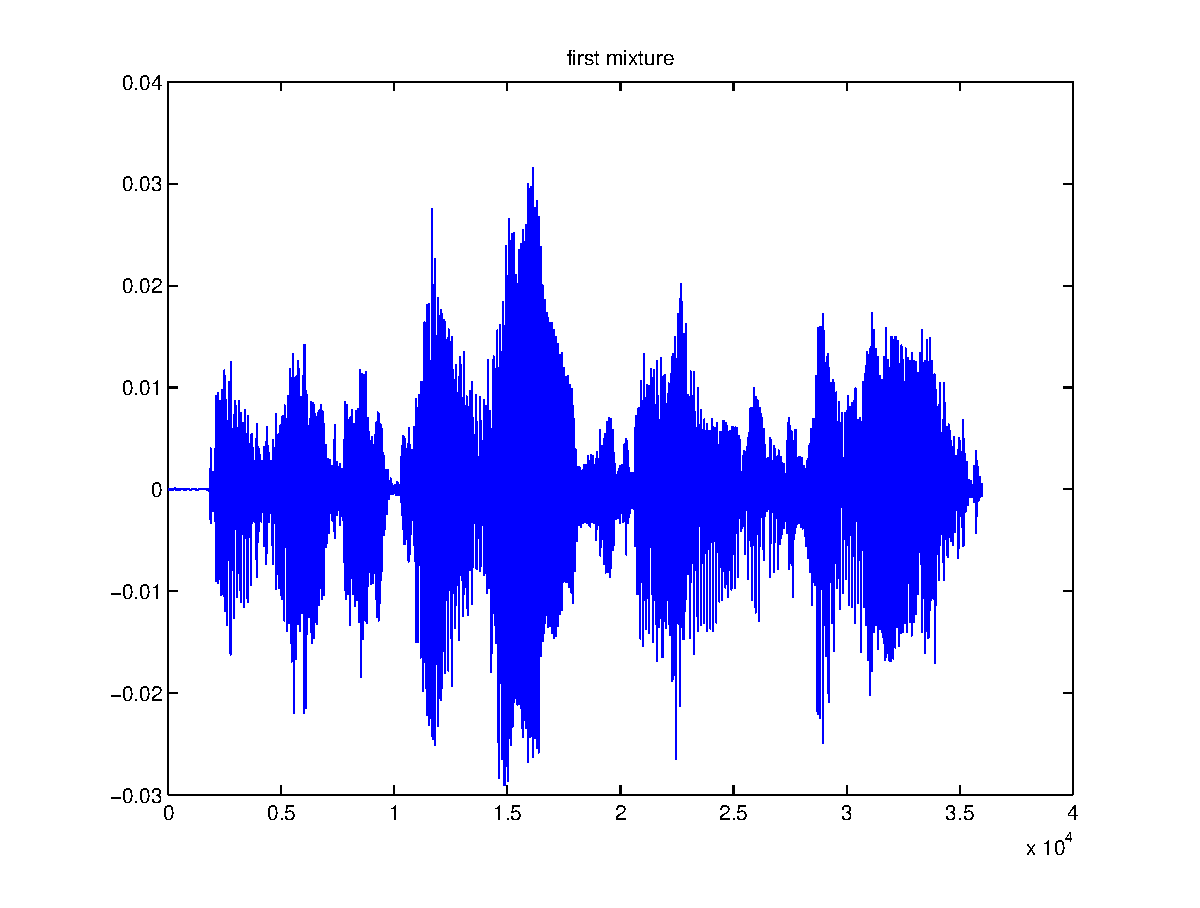
\includegraphics[width=0.4\textwidth]{8-Convolution-Case-Optimization/mixture-1.eps}
        }%
        \subfigure[Second Mixture]{%
           \label{fig:second}
           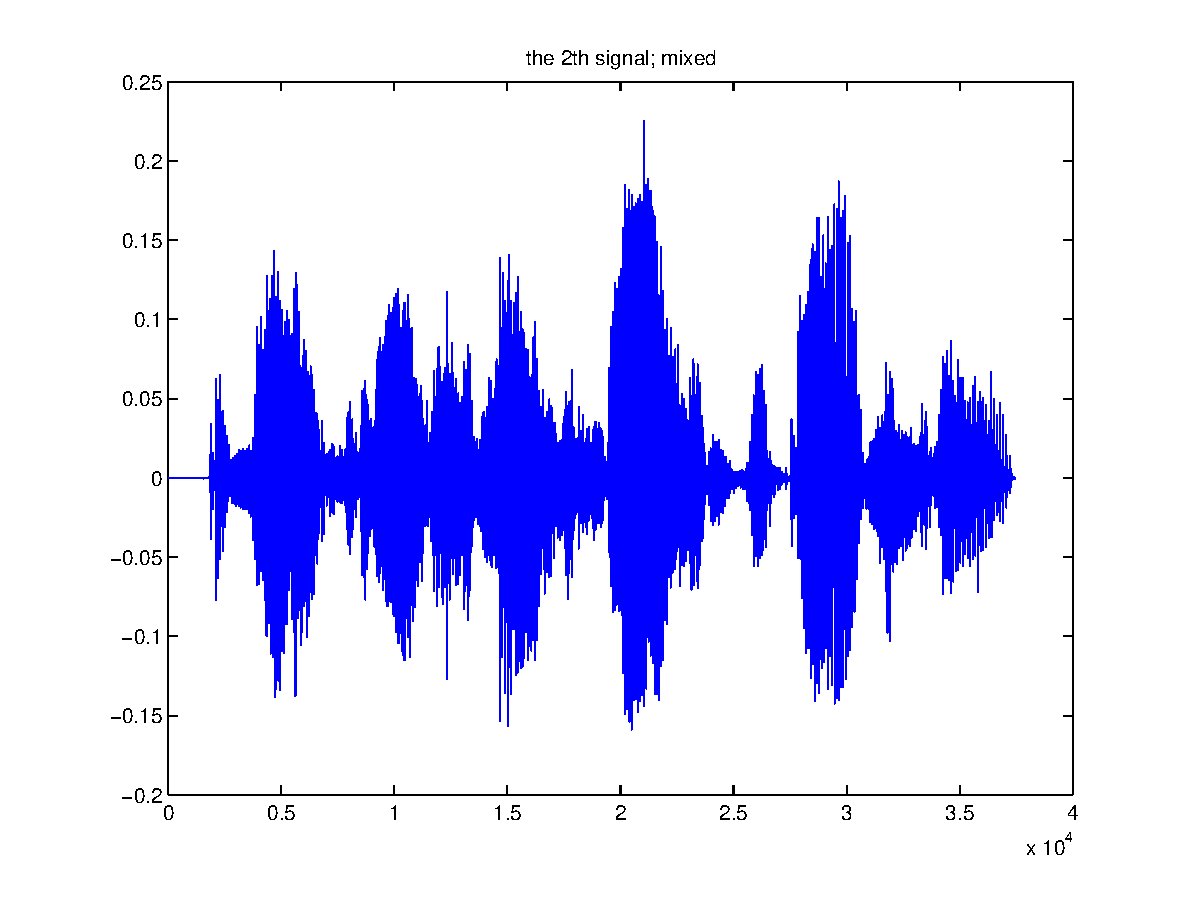
\includegraphics[width=0.4\textwidth]{8-Convolution-Case-Optimization/mixture-2.eps}
        } \\
 \subfigure[First Recovered Signal]{%
            \label{fig:first}
           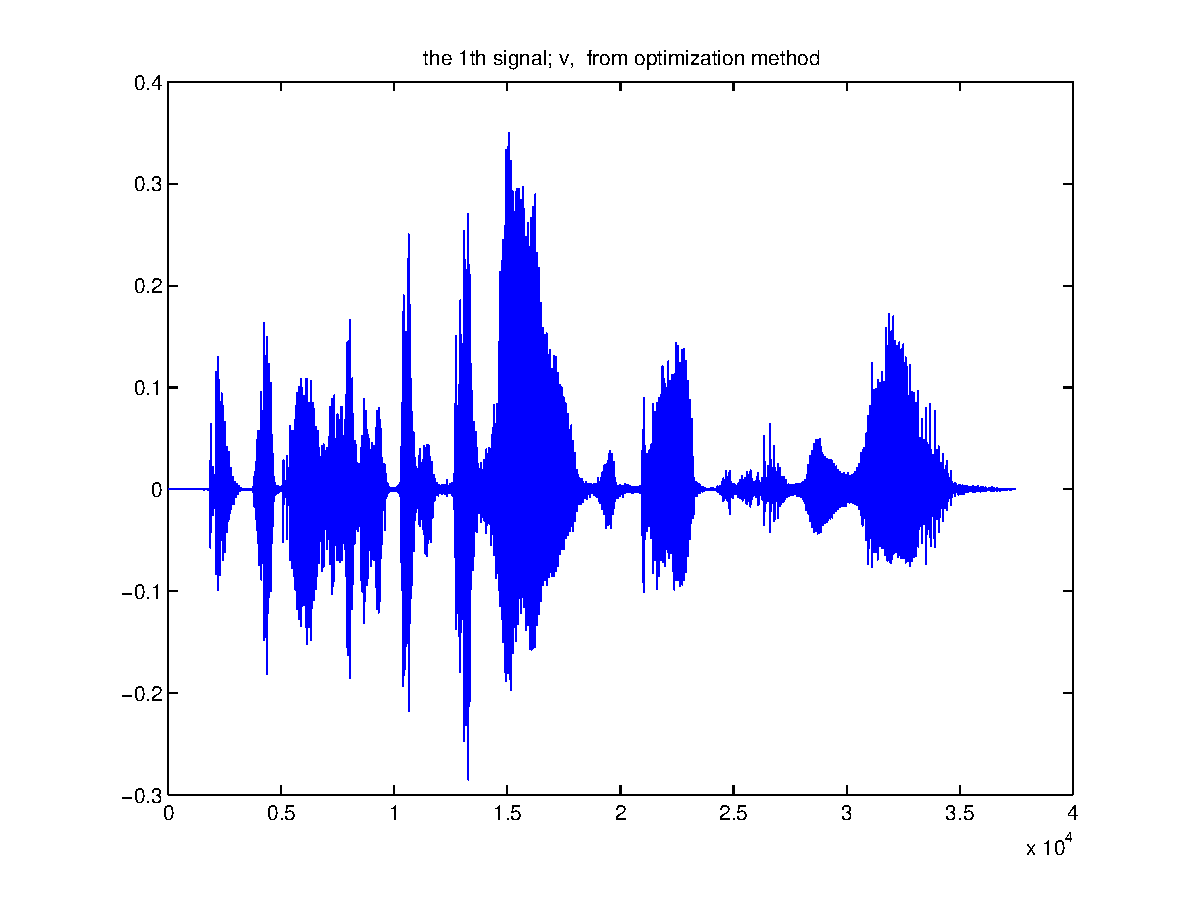
\includegraphics[width=0.4\textwidth]{8-Convolution-Case-Optimization/recovered-signal-1.eps}
        }%
        \subfigure[Second Recovered Signal]{%
           \label{fig:second}
            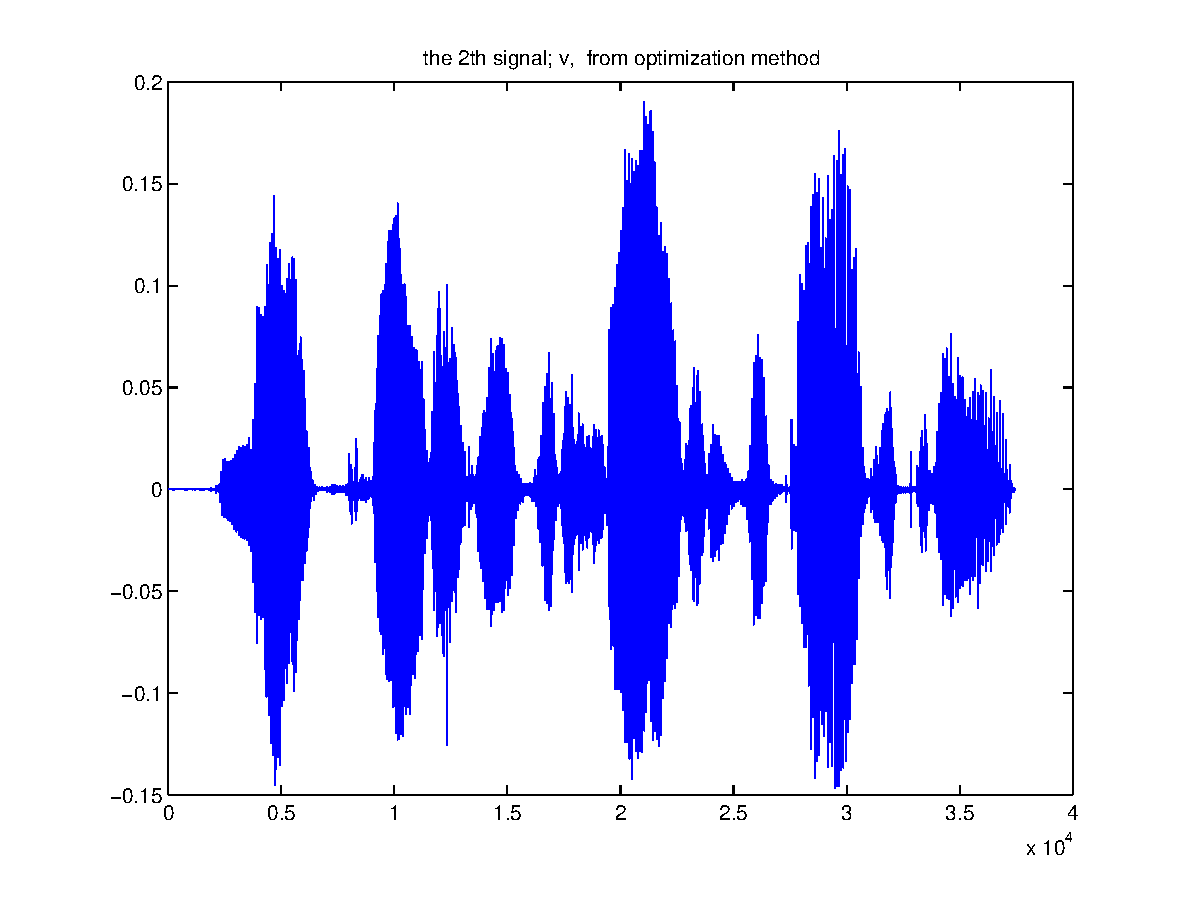
\includegraphics[width=0.4\textwidth]{8-Convolution-Case-Optimization/recovered-signal-2.eps}
        } 
        \subfigure[First Source Signal]{%
            \label{fig:first}
            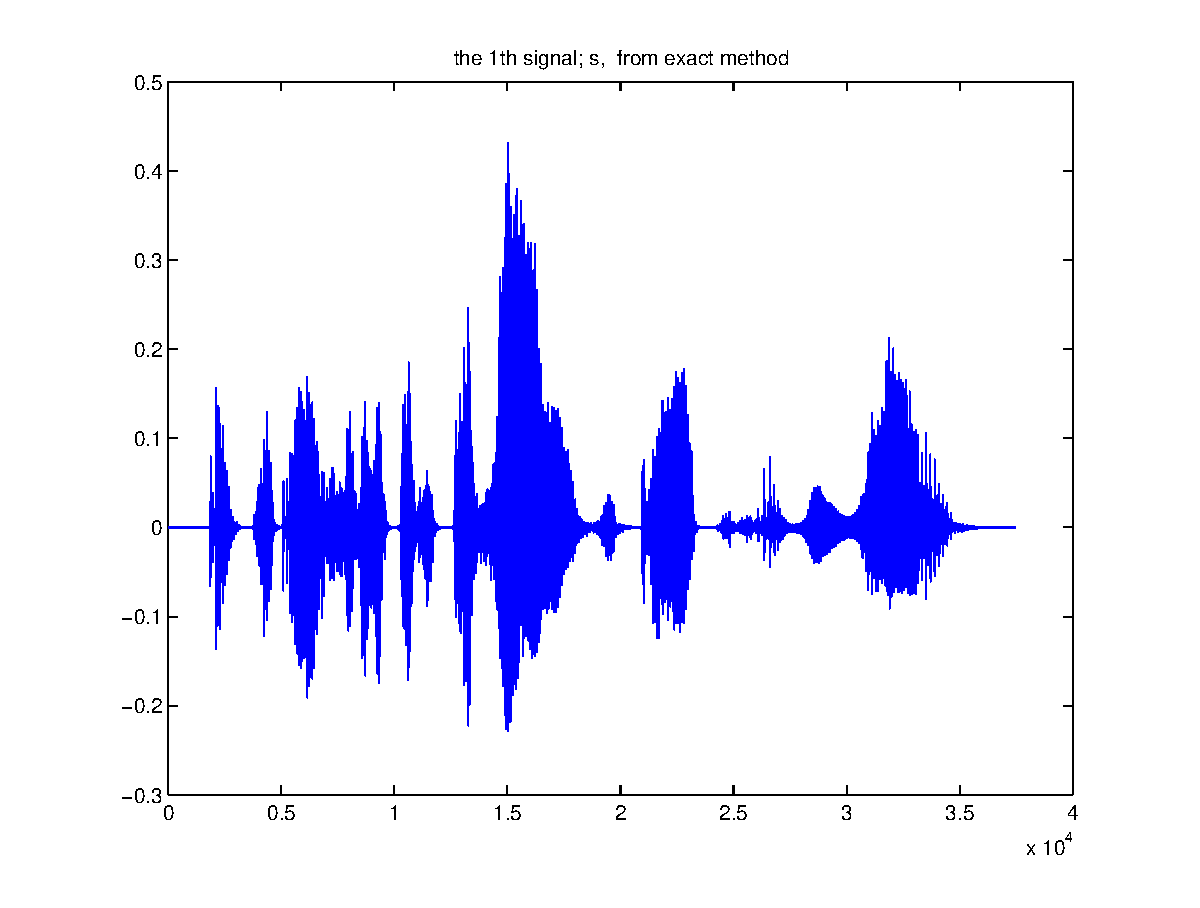
\includegraphics[width=0.4\textwidth]{8-Convolution-Case-Optimization/clean-signal-1.eps}
        }%
        \subfigure[Second Source Signal]{%
           \label{fig:second}
           \includegraphics[width=0.4\textwidth]{8-Convolution-Case-Optimization/clean-signal-2.eps}
        } \\

    \end{center}
    \caption{%
        This is the convolutive case using our global optimization method. %Note: because of complications in calculating the SIRI for the convolutive case, I use the $P$ matrix to determine the accuracy of my signal recoveries for convolutive cases.
Our global optimization method gives $sigmaP$ = 24.7826. 
%$P$ = [1.0000  0.0007; -0.0063  1.0000], $A0$ = [0.4545  0; 0  0.3846].
     }%
   \label{fig:subfigures}
\end{figure}

\vspace{0.1in}
\noindent
{\bf Example 5:}
Finally, we study the effect of using QR factorization in improving the performance of our global optimization method for degenerate measurements. We compare our method's performance with the Info-Max method's performance for one speech and one music signal mixed with noise in the degenerate case. Before applying QR, our method gives $sigmaP = 10.3$, while the Info-Max method gives $sigmaP = 2.2$. See the left subplot of Figure 8. Not applying QR, the global optimization algorithm converges extremely slowly, taking roughly four hours to complete the computation of 50 randomly generated mixing measurements. Often, we observed that the optimization stopped at a local minimum.

\begin{figure}
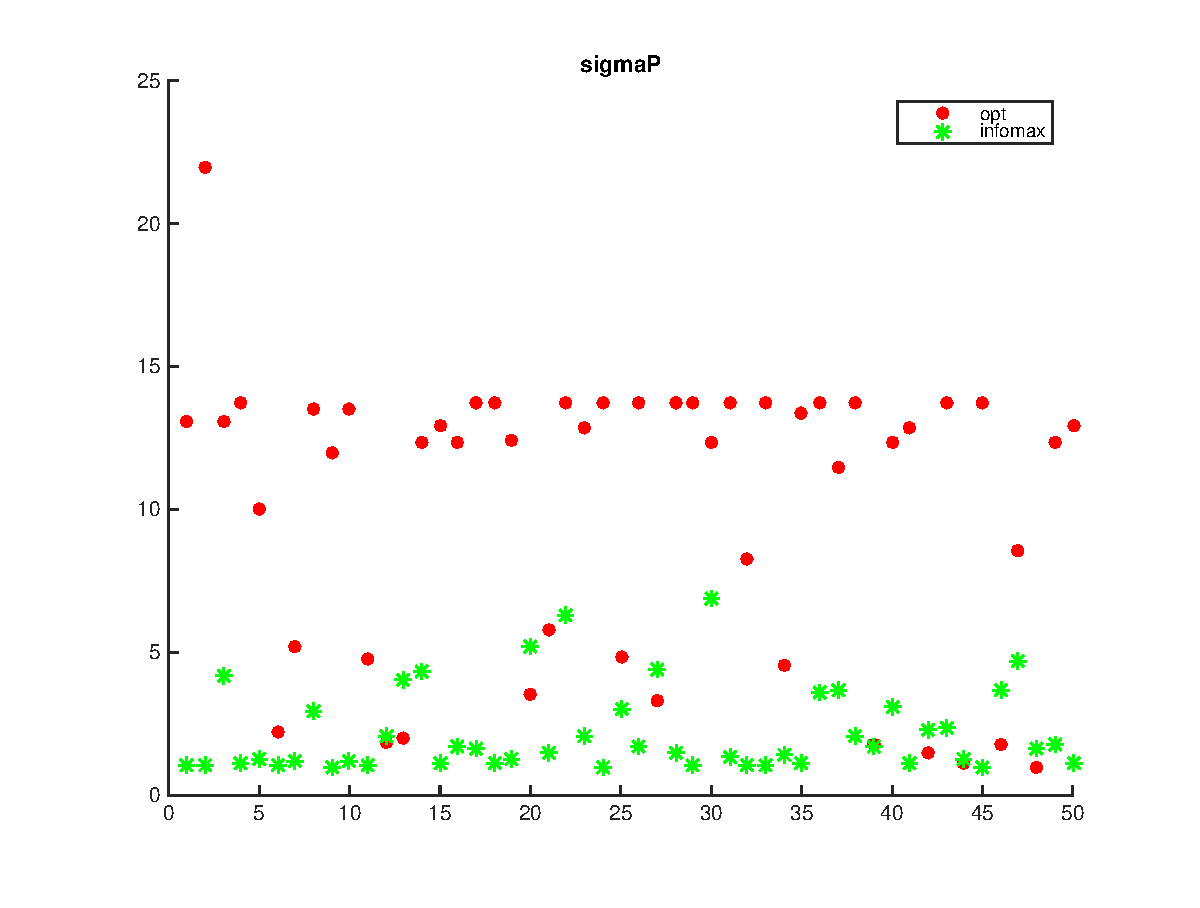
\includegraphics[scale=0.4]{0-Beijing/3by3_2sig1noise_deg/sigmaP-music-our-preQR.eps}
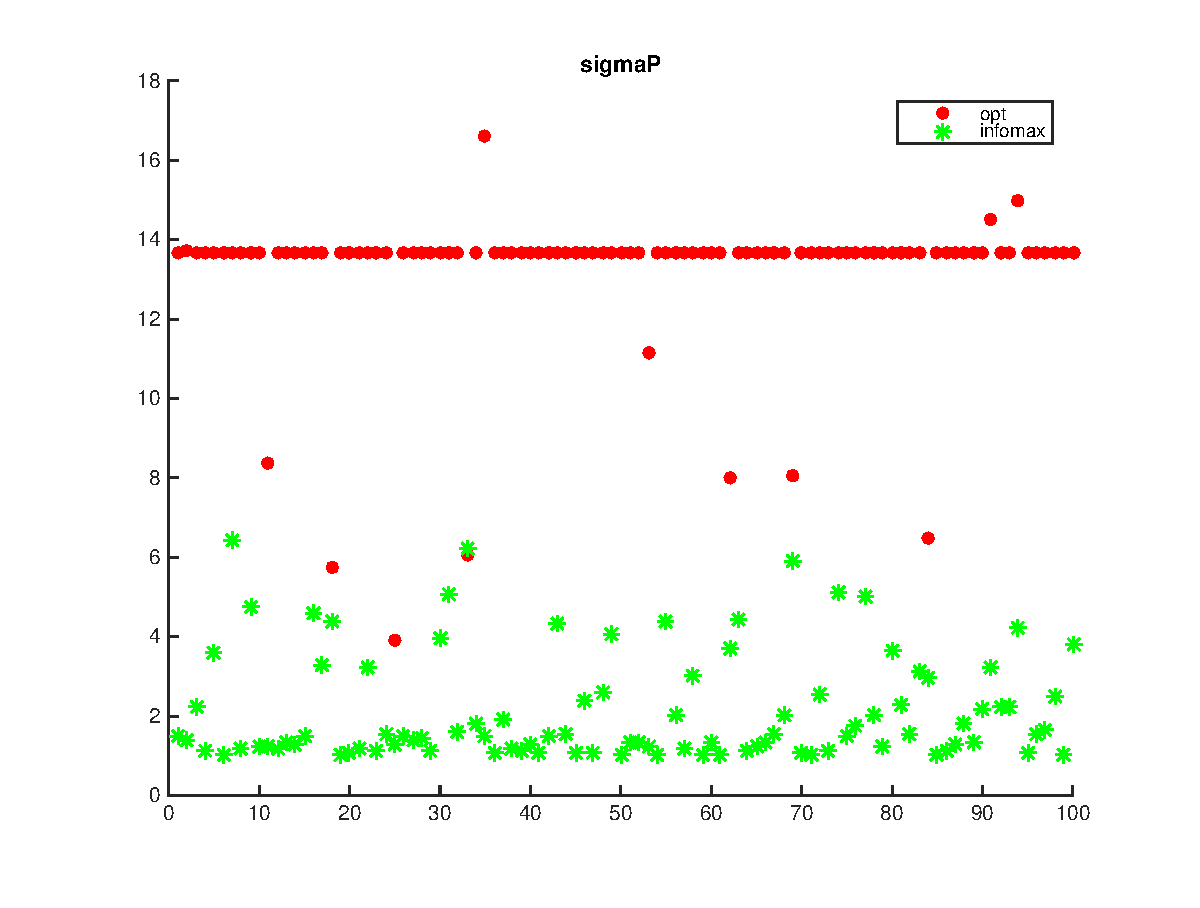
\includegraphics[scale=0.4]{0-Beijing/3by3_2sig1noise_deg/sigmaP-music-degen.eps}
\caption{One speech signal and one music signal mixed with noise in a degenerate setting. Comparison of our optimization method with the Info-Max method. Left subplot: Before applying QR, $sigmaP1 = 10.3$ and $sigmaP2= 2.2$. Right subplot: After applying QR, $sigmaP1 = 13.2$ and $sigmaP2= 2.2$.}
 \label{Example 4}

\end{figure}%

Next, we applied QR factorization to pre-process the degenerate measurements before implementing our global optimization method or the Info-Max method. The results with 100 randomly generated mixing matrices are plotted in the right subplot of Figure 8. We observed that the $sigmaP$ value improved for our method from 10.3 to 13.2, while the $sigmaP$ value for the Info-Max method remained the same. Moreover, we observed that the performance of our global optimization method is much more consistent after applying QR, whereas our method produces many outliers when we do not apply QR. These outliers correspond to the global optimization algorithm's stoppage at a local minimum, because we set a maximum number of iterations in the global optimization method. More importantly, after applying QR to the degenerate measurements, the global optimization algorithm converges much faster. It takes roughly 20 minutes to complete the computations of 100 randomly generated mixtures. The convergence of this case was 17 times quicker than the convergence of the case in which we did not apply QR factorization.

\section{Concluding Remarks}

Separating mixed signals in a noisy environment is known to be an extremely challenging problem, as existing blind source separation methods do not work effectively when the mixtures are polluted by noise. Traditional filtering methods such as low pass filter or wavelet filter tend to remove the high frequency information of the signals as well, thus resulting in a dissatisfactory recovery. However, by treating the noise as one of the source signals and obtaining an extra measurement, we proposed a simple global optimization method by minimizing the cross-correlation of the recovered signals. Our method works well in the instantaneous and convolutive cases. In both cases, we gave precise solvability conditions for our global optimization method. Moreover, we performed rigorous stability and error analysis in the realistic setting of source signals having small but non-zero correlation. To the best of our knowledge, we are the first to have provided a rigorous error analysis of BSS methods.

In some applications, the measurements are degenerate. This could be the case when one of the source signals is far away from the recording device, or when two recording devices are placed close together. Although the separation of source signals with nearly degenerate mixtures is difficult, by performing very careful estimates, we proved that our method can still give accurate recovery even when the mixing matrix is nearly degenerate in the two-signal setting. For the more general case, we proposed a new method based on the QR factorization to separate degenerate measurements. After pre-processing the measurements with the QR factorization, the corresponding mixing matrix becomes non-degenerate. Prior to applying the QR factorization, the energy functional is very flat near the global minimum, thus resulting in an extremely slow convergence in the global optimization algorithm. However, after applying the QR factorization to the degenerate mixtures, the energy wells become much steeper and the global optimization algorithm converges significantly faster and yields a more accurate recovery. 

Furthermore, we performed extensive numerical studies to demonstrate the robustness and accuracy of our method. By comparing our global optimization method with the analytic de-mixing method, and the Info-Max method, which uses higher order statistics, we demonstrated that our method performs better than the analytic method and the Info-Max method, especially when the mixtures are nearly degenerate. 

However, there is still room from improvement, as there are several unsettled issues that we intend on resolving in the near future. One common difficulty is associated with long convolution (strongly reverberant rooms). Due to the non-convex nature of our energy functional, our global optimization method does not converge fast enough to be competitive in realistic applications with long convolution. We plan to significantly speed up the global optimization algorithm and develop a fast and effective global minimization method that is tailored to our specific objective function. One possibility is to develop a randomized search algorithm, like simulated annealing, to solve the global minimization problem in the high dimensional setting of convolutional mixtures. 

Another difficulty is to handle signals that come from the same direction. An illustration would be one person standing in front of another. This corresponds to degenerate mixtures. The QR factorization method that we proposed is effective in transforming the energy functional into a much better distribution of energy wells with steep gradients. Our numerical results indicate that the multiple energy wells near the global minimum are actually global minima. Thus it is sufficient for the global minimization algorithm to locate any one of these global minimal wells. We plan to prove this property rigorously and extend this technique to other BSS methods.

Currently, none of the existing methods provides any error analysis. We intend on extending our method of analysis to other BSS methods that have been used widely in practice. Such analysis would provide important guidelines in  improving the performance of these methods.

In practice, we may always know the number of source signals in advance. If we have a prior estimate of the number of source signals that we would like to recover, we would need at least the same number of mixtures to recover them. If obtaining more mixtures than source signals were possible, we would have a better recovery. However, in the case when the number of mixtures is smaller than the number of source signals, we would treat the source signals that are closest to the recorders as the source signals that we intend to recover, and we would treat the remaining source signals as background noise. For example, if we place the recorders close together near our targeted signals and assume that the remaining signals are far from the recorders, then each recorder will roughly pick up the same background mixture. We could then treat this mixture as an independent noise signal. Thus my method would still successfully separate the targeted signals from the remote background source signals. If one can learn the intrinsic sparsity structure of the source signals and construct the corresponding sparse basis in the time frequency domain, then it is possible to recover all the source signals using only a smaller number of mixtures by using $L^1$ minimization. This is a topic that is under investigation.

Finally, we would like to explore the technological transfer of our method into practical applications. In particular, we would like to apply our method in designing a new generation of hearing aid devices. For such purposes, we would need at least two receivers to process the received mixtures simultaneously in order to separate the background noise from the targeted signal. And, to transmit the received mixtures to a remote central computer for the processing of data and the dispatching of recovered signals in real-time, we would need a wireless device. We also intend on creating a mobile application that connects the hearing aid device to a smartphone, which processes the mixtures in real-time. In fact, our error analysis has proven that the concept of such technology is plausible. If these efforts carry through, it may greatly help millions of senior citizens who suffer from the devastating effects of hearing loss.

\begin{thebibliography}{100} % 100 is a random guess of the total number of
%references

\bibitem{Bell95} A. Bell and T. Sejnowski, ``An Information-Maximization Approach to Blind Separation and
Blind Deconvolution'', Neural Computation, 7(1995), pp 1129-1159.

{\it The authors derive a new self-organizing learning algorithm that maximizes the information transferred in a network of nonlinear units.  The algorithm does not assume any knowledge of the input distributions, and is defined here for the zero-noise limit. The nonlinearities in the transfer function are able to pick up higher-order moments of the input distributions. This enables the network to separate statistically independent components in the inputs. This can be considered as a higher-order generalization of principal component analysis. The authors apply the network to the source separation (or cocktail party) problem, successfully separating unknown mixtures of up to 10 speakers.  Finally, the authors derive dependencies of information transfer on time delays. Their study suggests that information maximization provides an unifying framework for problems in "blind" signal processing.}


\bibitem{Cardoso93} J-F. Cardoso and A. Souloumiac, ``Blind beamforming for non-Gaussian signals'',
IEEE-Proceedings-F (Radar and Signal Processing), 140(6) (1993), pp. 362-370.

{\it This paper considers an application of blind identification to beamforming. The key point is to use estimates of directional vectors rather than resorting to their hypothesized value. By using estimates of the directional vectors obtained via blind identification, beamforming is made robust with respect to array deformations, distortion of the wave front, pointing errors, etc. so that neither array calibration nor physical modeling is necessary.  The authors exploit fourth-order cumulants to enforce the statistical independence of the sources, which is the key assumption in blind source identification. A computationally efficient technique is presented for the blind estimation of directional vectors, based on joint diagonalization of 4th-order cumulant matrices.}

\bibitem{Smaragdis98}P. Smaragdis, ``Blind separation of convolved mixtures in the frequency domain'',
Neurocomputing,  22(1-3) (1998), pp. 21-34.

{\it The author employs information theoretic algorithms, previously used for separating instantaneous mixtures of sources and for separating convolved mixing in the frequency domain. It is observed that convolved mixing in the time domain corresponds to instantaneous mixing in the frequency domain. Such mixing can be inverted using simpler and more robust algorithms than the ones recently developed. Advantages of this approach are improved efficiency and better convergence features.}

\bibitem{Steeb97}
W-H. Steeb, ``Matrix Calculus and Kronecker Product with Applications and C++ Programs '', World Scientific. Publ., October, 1997.

{\it The Kronecker product of matrices plays a central role in mathematics and in applications found in engineering and theoretical physics. These applications are signal processing, statistical physics, quantum groups and quantum computers. This book provides a comprehensive introduction to the Kronecker product of matrices, matrix calculus, tensor product and their applications. Another attractive feature of this book is that it provides software implementation of Kronecker product in C++ using an object-oriented design.}

\bibitem{Xin14} J. Xin and Y. Qi,
``Mathematical Modeling and Signal Processing in Speech and Hearing Sciences'', Modeling, Simulation \& Applications, Vol. 10, Springer publication, 2014.
    
{\it The aim of this book is to give an accessible introduction of mathematical models and signal processing methods in speech and hearing sciences for senior undergraduate and beginning graduate students with basic knowledge of linear algebra, differential equations, numerical analysis, and probability. This book has several attractive features.  It provides a user friendly and systematic introduction to mathematical models in speech and hearing sciences. Another feature is that it provides step-by-step analysis of models and computational methods from numerical analysis, signal processing, and statistics. Furthermore, it connects mathematics and computation with speech/hearing phenomena and signal processing. Last but not least, it provides hands-on MATLAB programs to simulate models and analyze data; results come quickly (most of them in seconds) for seeing and hearing, directly enhancing learning experience. Chapter 5 of the book is devoted to blind source separation methods.}

\bibitem{Yilmaz04} O. Yilmaz and S.Rickard, ``Blind separation of speech mixtures via time-frequency masking'',
IEEE Trans. Signal Processing, 52(7) (2004), 1830-1847.
    
{\it In this paper, the authors introduce the concept of approximate W-disjoint orthogonality. The results demonstrate that there exist ideal binary time-frequency masks that can separate several speech signals from one mixture. While determining these masks blindly from just one mixture is an open problem, the authors show that one can approximate the ideal masks in the case where two anechoic mixtures are provided. The authors define a power weighted two-dimensional histogram constructed from the ratio of the time-frequency representations of the mixtures that is shown to have one peak for each source with peak location corresponding to the relative attenuation and delay mixing parameters. The histogram is used to create time-frequency masks that partition one of the mixtures into the original sources. Experimental results on speech mixtures verify the technique.}

\end{thebibliography}

%\begin{thebibliography}{100} % 100 is a random guess of the total number of
%%references
%\bibitem{Boney96} Boney, L., Tewfik, A.H., and Hamdy, K.N., ``Digital
%Watermarks for Audio Signals," \emph{Proceedings of the Third IEEE
%International Conference on Multimedia}, pp. 473-480, June 1996.
%\bibitem{MG} Goossens, M., Mittelbach, F., Samarin, \emph{A LaTeX
%Companion}, Addison-Wesley, Reading, MA, 1994.
%\bibitem{HK} Kopka, H., Daly P.W., \emph{A Guide to LaTeX},
%Addison-Wesley, Reading, MA, 1999.
%\bibitem{Pan} Pan, D., ``A Tutorial on MPEG/Audio Compression," \emph{IEEE
%Multimedia}, Vol.2, pp.60-74, Summer 1998.
%\end{thebibliography}

\end{document}
